\newif\ifisarxiv
\isarxivtrue

% \documentclass{article}
\documentclass[thesis.tex]{subfiles}

% if you need to pass options to natbib, use, e.g.:
%     \PassOptionsToPackage{numbers, compress}{natbib}
% before loading neurips_2020

% ready for submission
% \usepackage{neurips_2020}

% to compile a preprint version, e.g., for submission to arXiv, add add the
% [preprint] option:
%     \usepackage[preprint]{neurips_2020}

% to compile a camera-ready version, add the [final] option, e.g.:
%     \usepackage[final]{neurips_2020}

% to avoid loading the natbib package, add option nonatbib:
\ifisarxiv
% \usepackage{fullpage}
% \usepackage{natbib}
% \else
% \usepackage[final]{neurips_2020}
% \fi
% \usepackage[utf8]{inputenc} % allow utf-8 input
% \usepackage[T1]{fontenc}    % use 8-bit T1 fonts
% \usepackage{hyperref}       % hyperlinks
% \usepackage{url}            % simple URL typesetting
% \usepackage{booktabs}       % professional-quality tables
% \usepackage{amsfonts}       % blackboard math symbols
% \usepackage{nicefrac}       % compact symbols for 1/2, etc.
% \usepackage{microtype}      % microtypography
%  \usepackage{subfigure}
% \usepackage{amsmath,amsthm}
% \usepackage{cancel}
% \usepackage{cleveref}
% \usepackage{mathtools}
% \usepackage{enumitem}
% \usepackage{todonotes}
% \usepackage{xcolor}
% \usepackage{xfrac}
% \usepackage{caption}
% \hypersetup{
% 	colorlinks,
% 	linkcolor={red!40!gray},
% 	citecolor={blue!40!gray},
% 	urlcolor={blue!70!gray}
% }
% \newcommand{\BLUE}{\color[rgb]{0,0,0.69}}
% \def\opt{{\textsc{OPT}_k}}
\def\const{{\mathrm{const}}}
\def\nnz{{\mathrm{nnz}}}
\def\r{\sfrac{\sigma_{\w}^2}{\sigma_{\xib}^2}}
\def\rm{\sfrac{\sigma_{\xib}^2}{\sigma_{\w}^2}}
\def\cmark{\Green{\checkmark}}
\def\xmark{\Red{\large\sffamily x}}
\newcommand{\pdet}{{\mathrm{pdet}}}
\newcommand{\MSPE}[1] {{\mathrm{MSPE}\big[#1\big]}}
\newcommand{\MSE}[1] {{\mathrm{MSE}\big[#1\big]}}
\def\Poisson{{\operatorname{Poisson}}}
\def\PB{{\operatorname{PB}}}
\newcommand{\DP}[1]{\mathcal{DP}^{#1}}
\def\Ic{\mathcal{I}}
\def\Jc{\mathcal{J}}
\def\Mc{\mathcal M}
\def\Ec{\mathcal E}
\def\sr{{\mathrm{sr}}}
\def\ktd{{k^{\underline{d}}}}
\def\Det{{\mathrm{Det}}}
\def\detu{{\widecheck{\mathrm{Det}}_\mu^\gamma}}
\def\deto{{\widehat{\mathrm{Det}}_\mu^\gamma}}
\def\Zu{{\widecheck{Z}_\mu^{\gamma}}}
\def\Zo{{\widehat{Z}_\mu^{\gamma}}}
\def\Zun{{\widecheck{Z}_\mu^{\gamma_n}}}
\def\Zon{{\widehat{Z}_\mu^{\gamma_n}}}
\newcommand{\Er}{\mathrm{Er}}
\newif\ifDRAFT
\DRAFTtrue
\ifDRAFT
\newcommand{\marrow}{\marginpar[\hfill$\longrightarrow$]{$\longleftarrow$}}
\newcommand{\niceremark}[3]
   {\textcolor{red}{\textsc{#1 #2:} \marrow\textsf{#3}}}
\newcommand{\ken}[2][says]{\niceremark{Ken}{#1}{#2}}
\newcommand{\manfred}[2][says]{\niceremark{Manfred}{#1}{#2}}
\newcommand{\michael}[2][says]{\niceremark{Michael}{#1}{#2}}
\newcommand{\michal}[2][says]{\niceremark{Michal}{#1}{#2}}
\newcommand{\feynman}[2][says]{\niceremark{Feynman}{#1}{#2}}
%\usepackage[inline]{showlabels}
\else
\newcommand{\ken}[1]{}
\newcommand{\michael}[1]{}
\newcommand{\michal}[1]{}
\newcommand{\feynman}[1]{}
\fi
\newcommand{\norm}[1]{{\| #1 \|}}

\newcommand{\deff}{d_{\textnormal{eff}}}
\def\ee{\mathrm{e}}
\newcommand\mydots{\makebox[1em][c]{.\hfil.\hfil.}}
\def\Sd{\mathscr{S}_{\!d}}
\newcommand{\dx}{\dxy_{\!\cal X}}
\newcommand{\dxk}{\dxy_{\!\cal X}^k}
\newcommand{\dk}{\dxy^k}
\newcommand{\dxy}{\mathrm{D}}
\def\simiid{\overset{\textnormal{\fontsize{6}{6}\selectfont
i.i.d.}}{\sim}}
%\newcommand{\Dxy}{D_{\!\cal X\!,\cal Y}}
\def\vskx{{\mathrm{VS}_{\!\dx}^k}}
\def\vsk{{\mathrm{VS}_{\!D}^k}}
\def\vskxm{{\mathrm{VS}_{\!\dx}^{k-1}}}
\def\vskm{{\mathrm{VS}_{\!D}^{k-1}}}
\def\vsdx{{\mathrm{VS}_{\!\dx}^d}}
\def\vsd{{\mathrm{VS}_{\!D}^d}}
\newcommand{\vs}[1]{{\mathrm{VS}_{\!D}^{#1}}}
\newcommand{\sigd}{\boldsymbol\Sigma_{\!\dx}}
\def\wols{\w_{\mathrm{LS}}}
\def\wds{\boldsymbol\w_{\!D}^*}
\def\kd{K_{\!\dx}}

\def\poly{{\mathrm{poly}}}
\def\polylog{{\mathrm{polylog}}}
\def\DPP{{\mathrm{DPP}}}
\def\DPPcor{{\DPP_{\!\mathrm{cor}}}}
\def\DPPens{{\DPP_{\!\mathrm{ens}}}}
\newcommand{\DPPreg}[1]{{\DPP_{\!\mathrm{reg}}^{#1}}}
\def\Vol{{\mathrm{VS}}}
\def\Lev{{\mathrm{Lev}}}
\newcommand\todod[1]{\Red{\# DH: #1}}
\newcommand{\explain}[2]{\mathrel{\overset{\makebox[0pt]{\text{\tiny
#1}}}{#2}}}
\def\tot {{\mathrm{tot}}}
\def\checkmark{\tikz\fill[scale=0.4](0,.35) -- (.25,0) --
(1,.7) -- (.25,.15) -- cycle;}
\newcommand{\mnote}[1]{{\bf\large \Magenta{*}}\marginpar{\small \Magenta{#1}}}
\newcommand{\bnote}[1]{{\bf #1}}

\newcommand{\sqrtshort}[1]{{\sqrt{\white{\Big|}\!\!\smash{\text{\fontsize{9}{9}\selectfont$#1$}}}}}
\newenvironment{proofof}[2]{\par\vspace{2mm}\noindent\textbf{Proof of {#1} {#2}}\ }{\hfill\BlackBox}
\newcommand{\sets}[2]
{{\hspace{-0.3mm}[\hspace{-0.3mm}#1\hspace{-0.3mm}]\hspace{-0.3mm}\choose
\hspace{-0.3mm}#2\hspace{-0.3mm}}}
\DeclareMathOperator{\sgn}{\textnormal{sgn}}
\DeclareMathOperator{\adj}{\textnormal{adj}}
\def\Rb{{\mathbf{R}}}
\DeclareMathOperator{\ws}{\widetilde{\w}}
\newcommand{\inote}[1]{{\bf {#1}}}
\def\xib{\boldsymbol\xi}
\def\Sigmab{\mathbf{\Sigma}}
\def\Sigmabh{\widehat{\Sigmab}}
\def\Sigmabt{\widetilde{\Sigmab}}
\def\S{\mathbf{S}}
\def\T{\mathbf{T}}
\def\xt{\tilde{x}}
\def\xbt{\widetilde{\x}}
\def\xbh{\widehat{\x}}
\def\ubh{\widehat{\u}}
\def\dom {{\mathrm{dom}}}
\def\val {{\mathrm{val}}}
\def\out {{\mathrm{out}}}
\def\iin  {{\mathrm{iin}}}
\def\s {\mathbf{s}}
\def\q {\mathbf{q}}
\def\qt{\tilde{q}}
\def\itld {j}
\def\ubt {\tilde{\u}}
\def\n{\{1..n\}}
\def\cb {\mathbf{c}}
\def\cW{\mathcal W}
\def\Xt{\widetilde{X}}
\def\Dbt{\widetilde{\D}}
\def\xtb{\tilde{\mathbf{x}}}
\def\ytb{\tilde{\mathbf{y}}}
\def\Xtb{\widetilde{\mathbf{X}}}
\def\Xbb{\overline{\X}}
\def\Xb{{\bar{\X}}}
\def\ybb{\overline{\y}}
\def\f{{\mathbf{f}}}
\def\g{{\mathbf{g}}}
\def\fbb{{\overline{\f}}}
\def\fb{{\overline{f}}}
\def\Xc{\mathcal{X}}
\def\W{\mathbf W}
\def\L{\mathbf{L}}
\def\Rb{\mathbf R}
\def\Pc{\mathcal{P}}
\def\Nc{\mathcal{N}}
\def\Pt{\widetilde{P}}
\def\Hc{\mathcal{H}}
\def\Wc{\mathcal{W}}
\def\Cc{\mathcal{C}}
\def\p{\mathbf p}
%\def\r{\mathbf r}
\def\Y{\mathbf Y}
\def\H{\mathbf H}
\def\K{\mathbf K}
\def\Kh{\widehat{K}}
\def\Kbh{{\widehat{\K}}}
\def\Q{\mathbf Q}
\def\Qbar{{\bar{\mathbf Q}}}
\def\Ytb{\widetilde{\mathbf{Y}}}
\def\c{{n-d\choose s-d}}
\DeclareMathOperator{\Proj}{Proj}
\newcommand{\Span}{\mathrm{span}}
\newcommand{\ofsubt}[1]{\mbox{\scriptsize \raisebox{0.25pt}{$(#1)$}}}
%\raisebox{0.5pt}{$($}}#1\mbox{\tiny \raisebox{0.5pt}{$)$}}}
\newcommand{\ofsub}[1]{\mbox{\small \raisebox{0.0pt}{$(#1)$}}}
%\newcommand{\ofsubb}[1]{\mbox{\footnotesize \raisebox{0.5pt}{$(#1)$}}}
%\newcommand{\ofsub}[1]{(#1)}
%\newcommand{\ofsub}[1]{\mbox{\tiny$|$\hspace{-0.5pt}\raisebox{-0.5pt}{$#1$}}}
\newcommand{\of}[2]{{#1{\!\ofsub{#2}}}}
\newcommand{\oft}[2]{{#1{\!\ofsubt{#2}}}}
\newcommand{\fof}[2]{{#1({#2})}}
\newcommand{\yof}[2]{{#1{\ofsub{#2}}}}
%\newcommand{\yofb}[2]{{#1{\ofsubb{#2}}}}
\newcommand{\lazy}{FastRegVol}
\newcommand{\volsamp}{RegVol}

\newcommand{\Sm}{{S_{-i}}}
\newcommand{\Sp}{{S_{+i}}}
\ifx\BlackBox\undefined
\newcommand{\BlackBox}{\rule{1.5ex}{1.5ex}}  % end of proof
\fi
%\renewcommand{\dagger}{+}
\DeclareMathOperator*{\argmin}{\mathop{\mathrm{argmin}}}
\DeclareMathOperator*{\argmax}{\mathop{\mathrm{argmax}}}
\DeclareMathOperator*{\diag}{\mathop{\mathrm{diag}}}
\def\x{\mathbf x}
\def\y{\mathbf y}
\def\ybh{\widehat{\mathbf y}}
\def\ybb{\bar{\mathbf y}}
\def\xbb{\bar{\mathbf x}}
\def\yb{{\bar y}}
\def\ybt{\widetilde{\mathbf y}}
\def\yh{\widehat{y}}
\def\yhb{\widehat{\y}}
\def\yt{\widetilde{y}}
\def\z{\mathbf z}
\def\a{\mathbf a}
\def\b{\mathbf b}
\def\w{\mathbf w}
\def\v{\mathbf v}
\def\m{\mathbf m}
\def\wbh{\widehat{\mathbf w}}
\def\wh{\widehat{\mathbf w}}
\def\vbh{\widehat{\mathbf v}}
\def\wbt{\widetilde{\mathbf w}}
\def\e{\mathbf e}
\def\zero{\mathbf 0}
\def\one{\mathbf 1}
\def\u{\mathbf u}
\def\ubbar{\bar{\mathbf u}}
\def\f{\mathbf f}
\def\ellb{\boldsymbol\ell}

\def\X{\mathbf X}
\def\Xs{\widetilde{\X}}
\def\B{\mathbf B}
\def\A{\mathbf A}
\def\C{\mathbf C}
\def\U{\mathbf U}
\def\Ubt{\widetilde{\mathbf U}}
\def\Ubh{\widehat{\mathbf U}}
\def\Ubbar{\bar{\mathbf U}}
\def\F{\mathbf F}
\def\D{\mathbf D}
\def\V{\mathbf V}
\def\M{\mathbf M}
\def\Mh{\widehat{\mathbf M}}
%\def\S{\mathbf S}
\def\Stb{\widetilde{\mathbf{S}}}
\def\Sbh{\widehat{\mathbf{S}}}
\def\St{\widetilde{\S}}
\def\Sh{\widehat{S}}
\def\Sc{\mathcal{S}}
\def\Fc{\mathcal{F}}
\def\Vc{\mathcal{V}}
\def\Bc{\mathcal{B}}
\def\Dc{\mathcal{D}}
\def\Z{\mathbf Z}
\def\Zbh{\widehat{\mathbf Z}}
\def\Zbt{\widetilde{\mathbf Z}}
\def\Abh{\widehat{\mathbf A}}
\def\I{\mathbf I}
\def\Ic{\mathcal I}
\def\II{\mathbf {I \!\,I}}
%\def\II{\boldsymbol {\mathbb I}}
\def\A{\mathbf A}
\def\P{\mathbf P}
\def\Ph{\widehat{\mathbf P}}
\def\cP{\mathcal P}
\def\cR{\mathcal R}
\def\Xt{\widetilde{\mathbf{X}}}
\def\Xh{\widehat{\mathbf{X}}}
\def\Rh{\widehat{R}}
\def\Ot{\widetilde{O}}
\def\At{\widetilde{\A}}


\def\E{\mathbb E}
\def\R{\mathbb R}
\def\N{\mathbb N}
\def\Pr{\mathrm{Pr}}
%\def\C{\mathbb C}
\def\tr{\mathrm{tr}}
\def\Sbar{{\bar{S}}}
\def\cS{{\mathcal{S}}}
\def\Tbar{{\bar{T}}}
\def\Tt{{\widetilde{T}}}
\def\rank{\mathrm{rank}}
\def\Prob{\mathrm{Prob}}
\def\Var{\mathrm{Var}}
\def\Xinv{(\X^\top\X)^{-1}}
\def\XinvS{(\X_S\X_S^\top)^{-1}}
\def\ABinvS{(\A_S\B_S^\top)^{-1}}
\def\ABinv{(\A\B^\top)^{-1}}
\def\xinv{\x_i^\top\Xinv\x_i}
\def\Xinvr{(\lambda\I+\X_{-1}^\top\X_{-1})^{-1}}
\def\pdet{\mathrm{pdet}}
\newcommand{\vol}{\mathrm{vol}}
%\newcommand{\defeq}{:=}
\newcommand{\defeq}{\stackrel{\textit{\tiny{def}}}{=}}
\newcommand{\di}{{[d+1]_{-i}}}
\newcommand{\cov}{\mathrm{cov}}
\let\origtop\top
\renewcommand\top{{\scriptscriptstyle{\origtop}}} % this makes transpose not so big

\definecolor{silver}{cmyk}{0,0,0,0.3}
\definecolor{yellow}{cmyk}{0,0,0.9,0.0}
\definecolor{reddishyellow}{cmyk}{0,0.22,1.0,0.0}
\definecolor{black}{cmyk}{0,0,0.0,1.0}
\definecolor{darkYellow}{cmyk}{0.2,0.4,1.0,0}
\definecolor{orange}{cmyk}{0.0,0.7,0.9,0}
\definecolor{darkSilver}{cmyk}{0,0,0,0.1}
\definecolor{grey}{cmyk}{0,0,0,0.5}
\definecolor{darkgreen}{cmyk}{0.6,0,0.8,0}
\newcommand{\Red}[1]{{\color{red}  {#1}}}
\newcommand{\Purple}[1]{{\color{purple}  {#1}}}
\newcommand{\Magenta}[1]{{\color{magenta}{#1}}}
\newcommand{\Green}[1]{{\color{darkgreen}  {#1}}}
\newcommand{\Blue}[1]{\color{blue}{#1}\color{black}}
\newcommand{\Orange}[1]{\textcolor{orange}{#1}\color{black}}
\newcommand{\Brown}[1]{{\color{brown}{#1}\color{black}}}
\newcommand{\Grey}[1]{{\color{grey}{#1}\color{black}}}
\newcommand{\white}[1]{{\textcolor{white}{#1}}}
\newcommand{\yellow}[1]{{\textcolor{reddishyellow}{#1}}}
\newcommand{\darkYellow}[1]{{\textcolor{darkYellow}{#1}}}
\newcommand{\grey}[1]{{\textcolor{grey}{#1}}}

\DeclareMathOperator{\half}{\frac{1}{2}}

\ifx\proof\undefined
\newenvironment{proof}{\par\noindent{\bf Proof\ }}{\hfill\BlackBox\\[2mm]}
\fi

\ifx\theorem\undefined
\newtheorem{theorem}{Theorem}
\fi

\ifx\example\undefined
\newtheorem{example}{Example}
\fi

\ifx\condition\undefined
\newtheorem{condition}{Condition}
\fi
\ifx\property\undefined
\newtheorem{property}{Property}
\fi

\ifx\lemma\undefined
\newtheorem{lemma}{Lemma}
\fi

\ifx\proposition\undefined
\newtheorem{proposition}{Proposition}
\fi

\ifx\remark\undefined
\newtheorem{remark}{Remark}
\fi

\ifx\corollary\undefined
\newtheorem{corollary}{Corollary}
\fi

\ifx\definition\undefined
\newtheorem{definition}{Definition}
\fi

\ifx\conjecture\undefined
\newtheorem{conjecture}{Conjecture}
\fi

\ifx\axiom\undefined
\newtheorem{axiom}{Axiom}
\fi

\ifx\claim\undefined
\newtheorem{claim}{Claim}
\fi

\ifx\assumption\undefined
\newtheorem{assumption}{Assumption}
\fi

\ifx\condition\undefined
\newtheorem{condition}{Condition}
\fi


\title{Precise expressions for random projections: \\
  Low-rank approximation and randomized Newton}

% The \author macro works with any number of authors. There are two commands
% used to separate the names and addresses of multiple authors: \And and \AND.
%
% Using \And between authors leaves it to LaTeX to determine where to break the
% lines. Using \AND forces a line break at that point. So, if LaTeX puts 3 of 4
% authors names on the first line, and the last on the second line, try using
% \AND instead of \And before the third author name.

\ifisarxiv
\author{
          \textbf{Micha{\l } Derezi\'{n}ski} \\
  Department of Statistics\\
  University of California, Berkeley\\
  \texttt{mderezin@berkeley.edu}\\
  \and
  \textbf{Feynman Liang} \\
  Department of Statistics\\
  University of California, Berkeley\\
  \texttt{feynman@berkeley.edu}
  \and
   \textbf{Zhenyu Liao} \\
  ICSI and Department of Statistics\\
  University of California, Berkeley\\
  \texttt{zhenyu.liao@berkeley.edu}
  \and
   \textbf{Michael W. Mahoney}\\
  ICSI and Department of Statistics\\
  University of California, Berkeley\\
  \texttt{mmahoney@stat.berkeley.edu}
}
\else
\author{%
 \textbf{Micha{\l } Derezi\'{n}ski} \\
  Department of Statistics\\
  University of California, Berkeley\\
  \texttt{mderezin@berkeley.edu}\\
  \And
  \textbf{Feynman Liang} \\
  Department of Statistics\\
  University of California, Berkeley\\
  \texttt{feynman@berkeley.edu}
  \And
   \textbf{Zhenyu Liao} \\
  ICSI and Department of Statistics\\
  University of California, Berkeley\\
  \texttt{zhenyu.liao@berkeley.edu}
  \And
   \textbf{Michael W. Mahoney}\\
  ICSI and Department of Statistics\\
  University of California, Berkeley\\
  \texttt{mmahoney@stat.berkeley.edu}
  % David S.~Hippocampus\thanks{Use footnote for providing further information
  %   about author (webpage, alternative address)---\emph{not} for acknowledging
  %   funding agencies.} \\
  % Department of Computer Science\\
  % Cranberry-Lemon University\\
  % Pittsburgh, PA 15213 \\
  % \texttt{hippo@cs.cranberry-lemon.edu} \\
  % examples of more authors
  % \And
  % Coauthor \\
  % Affiliation \\
  % Address \\
  % \texttt{email} \\
  % \AND
  % Coauthor \\
  % Affiliation \\
  % Address \\
  % \texttt{email} \\
  % \And
  % Coauthor \\
  % Affiliation \\
  % Address \\
  % \texttt{email} \\
  % \And
  % Coauthor \\
  % Affiliation \\
  % Address \\
  % \texttt{email} \\
}
\fi

\begin{document}
% \maketitle

% \begin{abstract}
It is often desirable to reduce the dimensionality of a large dataset
by projecting it onto a low-dimensional subspace.  Matrix sketching
has emerged as a powerful technique for performing such dimensionality
reduction very efficiently.  Even though there is an extensive
literature on the worst-case performance of sketching, existing
guarantees are typically very different from what is observed in
practice.  We exploit recent developments in the spectral analysis of
random matrices to develop novel techniques that provide provably
accurate expressions for the expected value of random projection
matrices obtained via sketching.  These expressions can be used to
characterize the performance of dimensionality reduction in a variety
of common machine learning tasks, ranging from low-rank approximation
to iterative stochastic optimization.  Our results apply to several
popular sketching methods, including Gaussian and Rademacher sketches,
and they enable precise analysis of these methods in terms of spectral
properties of the data.  Empirical results show that the expressions
we derive reflect the practical performance of these sketching
methods, down to lower-order effects and even constant factors. 
% \end{abstract}

\section{Introduction}
Many settings in modern machine learning, optimization and scientific
computing require us to work with data matrices that are so large that
some form of dimensionality reduction is a necessary component of the
process. One of the most popular families of methods for dimensionality reduction,
coming from the literature on Randomized Numerical Linear Algebra
(RandNLA), consists of data-oblivious sketches \cite{Mah-mat-rev_JRNL,tropp2011structure,woodruff2014sketching}. 
Consider a large $m\times n$
matrix $\A$. A \emph{data-oblivious sketch} of size $k$ is the matrix $\S\A$,
where $\S$ is a $k\times m$ random matrix such that
$\E[\frac1k\S^\top\S]=\I$, whose distribution does not
depend on $\A$. This sketch reduces the first dimension of $\A$ from
$m$ to a much smaller $k$ (we assume without loss of generality that
$k \ll n \le m$), and an analogous procedure can be defined for
reducing the second 
dimension as well. This approximate representation of $\A$ is central
to many algorithms in areas such as linear regression, low-rank approximation, kernel methods,
and iterative second-order optimization. While there is a long line of research
aimed at bounding the worst-case approximation error of such
representations, these bounds are often too loose to reflect accurately
the practical performance of these methods. In this paper, we develop new theory which
enables more precise analysis of the accuracy of sketched data
representations.

A common way to measure the accuracy of the sketch $\S\A$ is by
considering the $k$-dimensional subspace spanned by its rows. The goal
of the sketch is to choose a subspace that best aligns with the
distribution of all of the $m$ rows of $\A$ in $\R^n$. Intuitively, our goal
is to minimize the (norm of the) residual when projecting a vector $\a\in\R^n$ onto that
subspace, i.e., $\a - \P\a=(\I-\P)\a$, where
$\P = (\S\A)^\dagger\S\A$ is the orthogonal projection matrix onto the subspace
spanned by the rows of $\S\A$ (and $(\cdot)^\dagger$ denotes the
Moore-Penrose pseudoinverse). For this reason, the quantity that has appeared 
ubiquitously in the error analysis of RandNLA sketching is what we call the residual
projection matrix:
\begin{align*}
  \textbf{(residual projection matrix)}\quad \P_{\!\perp}\ :=\ \I - \P\ =\ \I
  - (\S\A)^\dagger\S\A.
\end{align*}
Since $\P_{\!\perp}$ is random, the average performance of the sketch
can often be characterized by its expectation, $\E[\P_{\!\perp}]$.
For example, the low-rank approximation error of the
sketch can be expressed as
$\E[\|\A - \A\P\|_F^2]= \tr\,\A^\top\A\,\E[\P_{\!\perp}]$, where
$\|\cdot\|_F$ denotes the Frobenius norm.  A similar formula follows for
the trace norm error of a sketched Nystr\"om approximation
\cite{Williams01Nystrom,revisiting-nystrom}.
Among others, this approximation error
appears in the analysis of sketched kernel 
ridge regression \cite{fanuel2020diversity} and Gaussian process
regression \cite{sparse-variational-gp}. Furthermore, a variety of
iterative algorithms, such as randomized second-order methods for
convex optimization \cite{Qu2015Feb,Qu2016,Gower2019,jacsketch}
and linear system solvers based on 
the generalized Kaczmarz method \cite{generalized-kaczmarz},
have convergence guarantees which depend on the extreme eigenvalues of
$\E[\P_{\!\perp}]$. Finally, a generalized form of the expected
residual projection has been recently used to model the implicit
regularization of the interpolating solutions in over-parameterized
linear models \cite{surrogate-design,BLLT19_TR}.

\subsection{Main result}
Despite its prevalence in the literature, the 
expected residual projection is not well understood, even in such
simple cases as when $\S$ is a Gaussian sketch (i.e., with
i.i.d.~standard normal entries). We address this by providing a
surrogate expression, i.e., a simple analytically
tractable approximation, for this matrix quantity:
\begin{align}
  \E[\P_{\!\perp}]\ \overset\epsilon\simeq \ \bar\P_{\!\perp}:=(\gamma\A^\top\A +
  \I)^{-1},\quad\text{with \ $\gamma>0$ \ s.t. \ }\tr\,\bar\P_{\!\perp} = n-k.\label{eq:surrogate}
\end{align}
Here, $\overset{\epsilon}{\simeq}$ means that while the surrogate expression is
not exact, it approximates the true quantity up to some $\epsilon$
accuracy. Our main result provides a rigorous approximation guarantee
for this surrogate expression with respect to a
range of sketching matrices $\S$, including the standard Gaussian and
Rademacher sketches. We state the result using the
positive semi-definite ordering denoted by $\preceq$. 
\begin{theorem}\label{t:main}
Let $\S$ be a sketch of size $k$ with i.i.d.~mean-zero sub-gaussian entries and let
  $r=\|\A\|_F^2/\|\A\|^2$ be the stable rank of $\A$.  If
  we let $\rho = r/k$ be a fixed constant larger than $1$, then
  \begin{align*}
    (1-\epsilon)\,\bar\P_{\!\perp}\preceq\E[\P_{\!\perp}]\preceq
    (1+\epsilon)\,\bar\P_{\!\perp}\quad\text{for}\quad \epsilon =
    O(\tfrac1{\sqrt r}).
  \end{align*}
\end{theorem}
In other words, when the sketch size $k$ is smaller than the stable rank $r$
of $\A$, then the discrepancy between our surrogate expression
$\bar\P_{\!\perp}$ and $\E[\P_{\!\perp}]$ is of the order
$1/\sqrt r$, where the big-O notation hides only the dependence
on $\rho$ and on the sub-gaussian constant (see Theorem \ref{t:main-tech} for
more details). Our proof of Theorem \ref{t:main} is inspired by the techniques from
random matrix theory which have been used to analyze the asymptotic
spectral distribution of large random matrices by focusing on the
associated matrix resolvents and Stieltjes transforms
\cite{hachem2007deterministic,bai2010spectral}. However, our analysis
is novel in several respects:
\begin{enumerate}
  \item The residual projection matrix can be obtained
    from the appropriately scaled resolvent matrix $z(\A^\top\S^\top\S\A+z\I)^{-1}$ by
    taking $z\rightarrow 0$. Prior work (e.g.,
      \cite{HMRT19_TR}) combined this with an exchange-of-limits argument to
      analyze the asymptotic behavior of the residual projection. 
      This approach, however, does not allow for a precise control in
      finite-dimensional problems. We are able to provide a more
      fine-grained, non-asymptotic analysis by working directly with
      the residual projection itself, instead of the resolvent.
  \item We require no assumptions on the largest and smallest singular
    value of $\A$. Instead, we derive our bounds in terms of the
    stable rank of $\A$ (as opposed to its actual rank), which
    implicitly compensates for ill-conditioned data matrices.
  \item We obtain upper/lower bounds for $\E[\P_{\!\perp}]$ in terms
    of the positive semi-definite ordering~$\preceq$, which can be
    directly converted to guarantees for the precise
    expressions of expected low-rank approximation error derived in
    the following section. 
    % are stronger than the standard error bounds
    % $\|\E[\P_{\!\perp}]-\bar\P_{\!\perp}\|$ because they lead to relative error
    % approximations for \emph{all} of the eigenvalues of
    % $\E[\P_{\!\perp}]$ (with respect to those of $\bar \P_{\!\perp}$).
  \end{enumerate}

It is worth mentioning that the proposed analysis is significantly
different from the sketching literature based on subspace
embeddings (e.g.,
\cite{sarlos-sketching,cw-sparse,nn-sparse,projection-cost-preserving,optimal-matrix-product}),
in the sense that here our object of interest is not to obtain
a worst-case approximation with high probability, but rather, our
analysis provides \emph{precise} characterization on the
\emph{expected} residual projection matrix that goes \emph{beyond
  worst-case bounds}. From an application perspective, the subspace
embedding property is neither sufficient nor necessary for many
numerical implementations of sketching \citep{blendenpik,lsrn}, 
or statistical results \citep{GarveshMahoney_JMLR,dobriban2019asymptotics,yang2020reduce}, as well as in the context of iterative optimization and implicit regularization (see Sections~\ref{s:newton}~and~\ref{s:implicit} below), which are discussed in detail as concrete applications of the proposed analysis.

\subsection{Low-rank approximation}
\label{s:low-rank}
We next provide some immediate corollaries of Theorem~\ref{t:main},
where we use $x\overset\epsilon\simeq y$ to denote a 
multiplicative approximation $|x-y|\leq \epsilon y$.
Note that our analysis is new even for the classical Gaussian sketch where
the entries of $\S$ are i.i.d.~standard normal. However the results
apply more broadly, including a standard class of data-base friendly
Rademacher sketches where each entry $s_{ij}$ is a $\pm1$ Rademacher
random variable \cite{achlioptas2003database}. We start by analyzing the Frobenius
norm error $\|\A-\A\P\|_F^2=\tr\,\A^\top\A\,\P_{\!\perp}$ of
sketched low-rank approximations. Note that by the definition of $\gamma$ in
\eqref{eq:surrogate}, we have $k =
\tr\,(\I-\bar\P_{\!\perp})=\tr\,\gamma\A^\top\A(\gamma\A^\top\A+\I)^{-1}$,
so the surrogate expression we obtain for the expected error is
remarkably simple.
\begin{corollary} %[low-rank approximation]
  \label{c:low-rank}
Let $\sigma_i$ be the singular values of $\A$. Under the assumptions of Theorem \ref{t:main}, we have:\vspace{-1mm}
  \begin{align*}
    \E\big[\|\A-\A\P\|_F^2\big] \ \overset\epsilon\simeq\ 
    k/\gamma
\quad \text{for \ $\gamma>0$ \ s.t. \ } \sum_{i}\frac{\gamma\sigma_i^2}{\gamma\sigma_i^2+1} = k.
%\quad \text{with \ $\gamma>0$ \ s.t. \ }\tr\,\gamma\A^\top\A(\gamma\A^\top\A+\I)^{-1} = k.
    % \tr\A^\top\A(\gamma\A^\top\A+\I)^{-1},
   % \quad \text{with \ $\gamma>0$ \ s.t. \ }\tr\,(\gamma\A^\top\A+\I)^{-1} = n-k.
  \end{align*}
\end{corollary}\vspace{-4mm}
\begin{remark}
  The parameter $\gamma=\gamma(k)$ increases at least linearly
  as a function of $k$, which is why the expected error will always
  decrease with increasing $k$. For example, when the singular values
  of $\A$ exhibit exponential decay, i.e., $\sigma_i^2=C\cdot\alpha^{i-1}$ for $\alpha\in(0,1)$, then the error also decreases
  exponentially, at the rate of $k/(\alpha^{-k}-1)$.
We discuss this further in Section \ref{s:explicit}, giving explicit
formulas for the error as a function of $k$ under both exponential and polynomial spectral
decay profiles.
\end{remark}
The above result is important for many RandNLA methods, and it is also relevant in the context of kernel methods,
where the data is represented via a positive semi-definite $m\times m$
kernel matrix $\K$ which corresponds to the matrix of dot-products of
the data vectors in some reproducible kernel Hilbert space. In this
context, sketching can be applied directly to the matrix $\K$ via an
extended variant of the
Nystr\"om method \cite{revisiting-nystrom}. A Nystr\"om approximation
constructed from a sketching matrix $\S$ is defined as $\tilde\K =
\C^\top\W^\dagger\C$, where $\C=\S\K$ and $\W=\S\K\S^\top$, and it is
applicable to a variety of settings, including Gaussian Process
regression, kernel machines and Independent
Component Analysis \cite{sparse-variational-gp,Williams01Nystrom,Bach2003}. By setting
$\A=\K^{\frac12}$, it is easy to see \cite{nystrom-multiple-descent} that
the trace norm error $\|\K-\tilde\K\|_*$ is identical to the squared
Frobenius norm error of the low-rank 
sketch $\S\A$, so Corollary \ref{c:low-rank} implies that
\begin{align}
  \E\big[\|\K-\tilde\K\|_*\big] \ \overset\epsilon\simeq\  k/\gamma \quad \text{for \ $\gamma>0$ \ s.t. \ } \sum_{i}\frac{\gamma\lambda_i}{\gamma\lambda_i+1} = k,\label{eq:nystrom}
\end{align}
with any sub-gaussian sketch, where $\lambda_i$ denote the
eigenvalues of $\K$. Our error analysis 
given in Section \ref{s:explicit} is particularly relevant here, since
commonly used kernels such as the Radial 
Basis Function (RBF) or the Mat\'ern kernel induce a well-understood eigenvalue
decay \cite{Santa97Gaussianregression,RasmussenWilliams06}.

Metrics other than the aforementioned Frobenius norm error,
such as the spectral norm error \cite{tropp2011structure}, are also of significant
interest in the low-rank approximation literature. We leave these
directions for future investigation.

\subsection{Randomized iterative optimization}
\label{s:newton}
We next turn to a class of iterative methods which take
advantage of sketching to reduce the per iteration cost of
optimization. These methods have been developed in a variety of
settings, from solving linear systems to convex optimization and
empirical risk minimization, and in many cases
the residual projection matrix appears as a black box quantity whose spectral
properties determine the convergence behavior of the algorithms
\cite{generalized-kaczmarz}. With
our new results, we can precisely characterize not only the rate of
convergence, but also, in some cases, the complete evolution of
the parameter vector, for the following algorithms:
% The following algorithms
% benefit from our improved convergence analysis:
\begin{enumerate}
  \item \emph{Generalized Kaczmarz method}
    \cite{generalized-kaczmarz} for approximately solving a linear system $\A\x=\b$;
  \item \emph{Randomized Subspace Newton} \cite{Gower2019}, a second order
    method, where we sketch the Hessian matrix.
  \item \emph{Jacobian Sketching} \cite{jacsketch}, a
    class of first order methods which use additional information via a
    weight matrix $\W$ that is sketched at every iteration.
    % \item \emph{Iterative Adaptive Sketching} \cite{lacotte2019high},
    %   a second order method where the sketching matrices are
    %   adaptively rescaled to improve the convergence rate.
      % \footnote{While
      %   \cite{lacotte2019high} also use the residual projection in
      %   their analysis, adapting our techniques is less
      %   straightforward in this case.}
\end{enumerate}
 We believe that
extensions of our techniques will apply to other algorithms,
such as that of \cite{lacotte2019high}. 

We next 
%Next, we 
give a result in the context of linear systems
for the generalized Kaczmarz method \cite{generalized-kaczmarz}, but a similar
convergence analysis is given for the methods of
\cite{Gower2019,jacsketch} in Appendix~\ref{a:newton}.
\begin{corollary}\label{c:kaczmarz}
Let $\x^*$ be the unique solution of $\A\x^*=\b$ and consider
  the iterative algorithm:
  \begin{align*}
    \x^{t+1} = \argmin_\x\|\x-\x^t\|^2\quad\textnormal{subject to}\quad\S\A\x=\S\b.
  \end{align*}
Under the assumptions of Theorem \ref{t:main}, with $\gamma$ defined in
\eqref{eq:surrogate} and $r=\|\A\|_F^2/\|\A||^2$, we have:
  \begin{align*}
    \E\big[\x^{t+1}-\x^*\big] \overset\epsilon\simeq 
    (\gamma\A^\top\A+\I)^{-1}\,\E\big[\x^t-\x^*\big]
    \quad\text{for}\quad\epsilon=O(\tfrac1{\sqrt r}). 
  \end{align*}
\end{corollary}
The corollary follows from Theorem \ref{t:main} combined with Theorem
4.1 in \cite{generalized-kaczmarz}. 
Note that when $\A^\top\A$ is positive definite then
$(\gamma\A^\top\A+\I)^{-1}\prec\I$, so the algorithm will
converge from any starting point, and the worst-case convergence rate of the above method can be
obtained by evaluating the largest eigenvalue of
$(\gamma\A^\top\A+\I)^{-1}$. However the result itself is much
stronger, in that it can be used to describe the (expected) trajectory of the
iterates for any starting point $\x^0$. Moreover, when the spectral decay
profile of $\A$ is known, then the explicit expressions for $\gamma$
as a function of $k$ derived in Section \ref{s:explicit} can be used
to characterize the convergence properties of generalized Kaczmarz as
well as other methods discussed above.

\subsection{Implicit regularization}\label{s:implicit}
%\paragraph{Implicit regularization.}

Setting $\x^t=\zero$, we can view one step of the iterative method in Corollary~\ref{c:kaczmarz} as
  finding a minimum norm interpolating solution of an under-determined linear
  system $(\S\A,\S\b)$. Recent interest in the generalization
capacity of over-parameterized machine learning models has
  motivated extensive research on the statistical properties of such interpolating
  solutions \cite[e.g.,][]{BLLT19_TR,HMRT19_TR,surrogate-design}. In this
  context, Theorem \ref{t:main} provides new evidence for the implicit
  regularization conjecture posed by \cite{surrogate-design} (see
  their Theorem 2 and associated discussion), with the amount of
  regularization equal $\frac1\gamma$, where $\gamma$ is implicitly
  defined in \eqref{eq:surrogate}: 
  \begin{align*}
  \underbrace{\E\Big[\argmin_\x\|\x\|^2\ \ \textnormal{s.t.}\ \
    \S\A\x=\S\b\Big] - \x^*}_{\text{Bias of sketched minimum norm solution}}
    \  \ \overset\epsilon\simeq\ \
    \underbrace{\argmin_\x\Big\{\|\A\x-\b\|^2+\tfrac1\gamma\|\x\|^2\Big\}
    - \x^*}_{\text{Bias of $l_2$-regularized solution}}.
  \end{align*}
While implicit regularization has received attention recently in the context of SGD algorithms for overparameterized machine learning models, it was originally discussed in the context of approximation algorithms more generally~\cite{Mah12}.
Recent work has made precise this notion in the context of RandNLA \cite{surrogate-design}, and our results here can be viewed in terms of implicit regularization of scalable RandNLA methods.


%\section{Related work}
\subsection{Related work}

A significant body of research has been dedicated to understanding the
guarantees for low-rank approximation via sketching,
particularly in the context of 
RandNLA \cite{DM16_CACM,RandNLA_PCMIchapter_chapter}. This line of work includes
i.i.d.~row sampling methods \cite{BoutsidisMD08,ridge-leverage-scores} which 
preserve the structure of the data, and data-oblivious methods such as
Gaussian and Rademacher sketches \cite{Mah-mat-rev_JRNL,tropp2011structure,woodruff2014sketching}. However,
all of these results focus on worst-case 
upper bounds on the approximation error. One exception is a recent
line of works on non-i.i.d.~row sampling with Determinantal Point Processes
(DPP, \cite{dpps-in-randnla}). In this case, exact analysis of the low-rank approximation
error \cite{nystrom-multiple-descent}, as well as precise convergence analysis
of stochastic second order methods \cite{randomized-newton}, have been
obtained. Remarkably, the expressions they obtain are analogous to
\eqref{eq:surrogate}, despite using completely different techniques. However, their analysis
is limited only to DPP-based sketches, which are considerably more
expensive to construct and thus much less widely used. The connection
between DPPs and Gaussian sketches was recently explored by 
\cite{surrogate-design} in the context of analyzing the implicit
regularization effect of choosing a minimum norm solution in
under-determined linear regression. They conjectured that the
expectation formulas obtained for DPPs are a good proxy for the
corresponding quantities obtained under a Gaussian
distribution. Similar observations were made by
\cite{debiasing-second-order} in the context of sketching for
regularized least squares and second order optimization. While
both of these works only provide empirical evidence for this
particular claim, our Theorem \ref{t:main} can be 
viewed as the first theoretical non-asymptotic justification of that
conjecture.

The effectiveness of sketching has also been extensively studied in
the context of second order optimization. These methods differ
depending on how the sketch is applied to the Hessian matrix, and
whether or not it is applied to the gradient as well. The class of
methods discussed in Section \ref{s:newton}, including Randomized
Subspace Newton and the Generalized Kaczmarz method, relies on
projecting the Hessian downto a low-dimensional subspace, which makes our
results directly applicable. A related family of methods uses
the so-called Iterative Hessian Sketch (IHS) approach \cite{pilanci2016iterative,lacotte2019faster}. The
similarities between IHS and the Subspace Newton-type methods (see
\cite{Qu2015Feb} for a comparison) suggest that our techniques could be
extended to provide precise convergence guarantees also to the IHS.
Finally, yet another family of Hessian sketching methods has been studied by
\cite{roosta2019sub,sketched-ridge-regression,XRM17_theory_TR,YXRM18_TR,fred_newtonMR_TR,distributed-newton,determinantal-averaging}.
These methods  preserve the  rank of the 
 Hessian, and so their convergence
guarantees do not rely on the residual projection.



\section{Precise analysis of the residual projection}

In this section, we give a detailed statement of our main technical
result, along with a sketch of the proof. First, recall the definition of
sub-gaussian random variables and vectors.
\begin{definition}
We say that $x$ is a
$K$-sub-gaussian random variable if its sub-gaussian Orlicz norm $\| x
\|_{\psi_2} \le K$, where $\| x \|_{\psi_2} := \inf\{ t > 0:~\E[
\exp(x^2/t^2) ] \le 2 \}$. Similarly, we say that a random vector $\x$ is
$K$-sub-gaussian if for all $\|\a\| \leq 1$ we have % that $\x^\top
% \a$ is a sub-gaussian random variable with
$\|\x^\top \a \|_{\psi_2} \leq K$.
\end{definition}

For convenience, we state the main result in a slightly different form than Theorem
\ref{t:main}. Namely, we replace the $m\times n$ matrix $\A$ with a  positive semi-definite
$n\times n$ matrix
$\Sigmab^{\frac12}$. Furthermore, instead of a sketch $\S$ with
i.i.d.~sub-gaussian entries, we use a random matrix $\Z$ with
i.i.d.~sub-gaussian \emph{rows}, which is a strictly weaker condition
because it allows for the entries of each row to be correlated. Since
the rows of $\Z$ are also assumed to have mean zero and identity covariance,
each row of $\Z\Sigmab^{\frac12}$ has covariance $\Sigmab$. In
Section \ref{s:reduction} we show how to 
convert this statement back to the form of Theorem~\ref{t:main}.

\begin{theorem}\label{t:main-tech}
Let $\P_\perp = \I - \X^\dagger \X$ for $\X = \Z\Sigmab^{\frac12}$,
where $\Z \in \mathbb R^{k\times n}$ has i.i.d.~$K$-sub-gaussian rows with zero mean and identity covariance, and
$\Sigmab$ is an $n\times n$ positive semi-definite matrix. Define:
\ifisarxiv\vspace{-1.25mm}\fi
\begin{align*}
\bar\P_\perp= (\gamma\Sigmab + \I)^{-1},\quad\text{such that}\quad\tr\,\bar\P_\perp=n-k.
\end{align*}
\ifisarxiv\vspace{-4.75mm}

\noindent
\fi
Let $r =\tr(\Sigmab)/\|\Sigmab\|$
be the stable rank of
$\Sigmab^{\frac12}$ and fix $\rho=r/k > 1$. There exists a constant
$C_{\rho}>0$, depending only on $\rho$ and $K$, such that if $r\geq
C_\rho$, then
\ifisarxiv\vspace{-1.5mm}\fi
\begin{align}
\Big(1-\frac {C_\rho}{\sqrt
  r}\Big)\cdot\bar\P_\perp\preceq\E[\P_\perp]\preceq
  \Big(1+\frac {C_\rho}{\sqrt r}\Big)\cdot\bar\P_\perp.
\end{align}
\end{theorem}

We first provide the following informal derivation of the expression for $\bar \P_\perp$
given in Theorem~\ref{t:main-tech}. 
% Let us use $\P$ to denote the matrix $\X^\dagger \X=\I-\P_{\perp}$. Using a 
% rank-one update formula for the Moore-Penrose pseudoinverse (see
% Lemma~\ref{l:rank-one-update} in the appendix) we have $\E[\P] = \E\big[(\X^\top \X)^\dagger \X^\top \X\big]= \sum_{i=1}^k \E[(\X^\top \X)^\dagger \x_i \x_i^\top]  = k\, \E\! \left[\frac{ (\I - \P_{-k}) \x_k \x_k^\top }{ \x_k^\top (\I - \P_{-k}) \x_k } \right]$, where we use $\x_i^\top$ to denote the $i$-th row of $\X$, and
% $\P_{-k} = \X_{-k}^\dagger \X_{-k} $, where $\X_{-i} $ is the matrix
% $\X$ without its $i$-th row. Due to the 
% sub-gaussianity of $\x_k$, the quadratic form $\x_k^\top (\I -
% \P_{-k}) \x_k$ in the denominator is expected to concentrate around
% its expectation (with respect to $\x_k$) and thus $\E[\X^\dagger \X] \simeq k\, \E\! \left[\frac{ (\I - \P_{-k}) \x_k \x_k^\top }{ \tr \Sigmab (\I - \P_{-k}) } \right] = k\E \left[\frac{ (\I - \P_{-k}) \Sigmab }{ \tr \Sigmab (\I - \P_{-k}) } \right]$, where we use $\E[\x_k \x_k^\top] = \Sigmab$. Further note that, with
% $\P_{-k} \simeq \P$ for large $k$ and $\frac1k \tr \Sigmab (\I -
% \P_{-k}) \simeq \frac1k \tr \Sigmab \E[\P_\perp]$ from a concentration
% argument, we conclude that $\E[\X^\dagger \X] = \I - \E[\P_\perp] \simeq \frac{ k \E[\P_\perp] \Sigmab }{ \tr \Sigmab \E[\P_\perp] }$, from which it follows that $\E[\P_\perp] \simeq  \big( \frac{ k\Sigmab}{ \tr \Sigmab \E[\P_\perp] } + \I \big)^{-1}$, and thus $\E[\P_\perp] \simeq \bar \P_\perp$ for $\bar \P_\perp =
% (\gamma \Sigmab + \I)^{-1}$ and $\gamma^{-1} = \frac1k \tr \Sigmab
% \bar \P_\perp$. This leads to the (implicit) expression for $\bar
% \P_\perp$ and $ \gamma$ given in Theorem \ref{t:main-tech}.  
Let us use $\P$ to denote the matrix $\X^\dagger \X=\I-\P_{\perp}$. Using a 
rank-one update formula for the Moore-Penrose pseudoinverse (see
Lemma~\ref{l:rank-one-update} in the appendix) we have
\[\I-\E[\P_{\perp}]=\E[\P] = \E\big[(\X^\top \X)^\dagger \X^\top \X\big]= \sum_{i=1}^k
  \E[(\X^\top \X)^\dagger \x_i \x_i^\top]  = k\, \E\! \left[\frac{ (\I
      - \P_{-k}) \x_k \x_k^\top }{ \x_k^\top (\I - \P_{-k}) \x_k }
  \right],\]
where we use $\x_i^\top$ to denote the $i$-th row of $\X$, and
$\P_{-k} = \X_{-k}^\dagger \X_{-k} $, where $\X_{-i} $ is the matrix
$\X$ without its $i$-th row. Due to the 
sub-gaussianity of $\x_k$, the quadratic form $\x_k^\top (\I -
\P_{-k}) \x_k$ in the denominator concentrates around
its expectation (with respect to $\x_k$), i.e., $\tr\Sigmab(\I-\P_{-k})$,
% and thus $\E[\P] \simeq k\, \E\! \left[\frac{ (\I - \P_{-k}) \x_k \x_k^\top }{ \tr \Sigmab (\I - \P_{-k}) } \right] = k\E \left[\frac{ (\I - \P_{-k}) \Sigmab }{ \tr \Sigmab (\I - \P_{-k}) } \right]$,
where we use $\E[\x_k \x_k^\top] = \Sigmab$. Further note that, with
$\P_{-k} \simeq \P$ for large $k$ and $\frac1k \tr \Sigmab (\I -
\P_{-k}) \simeq \frac1k \tr \Sigmab \E[\P_\perp]$ from a concentration
argument, we conclude~that
\begin{align*}
\I - \E[\P_\perp] \simeq \frac{ k \E[\P_\perp] \Sigmab }{
  \tr \Sigmab \E[\P_\perp] }\qquad\Longrightarrow\qquad \E[\P_\perp] \simeq  \Big( \frac{ k\Sigmab}{ \tr \Sigmab \E[\P_\perp] } + \I \Big)^{-1},
\end{align*}
  % from which it follows that $\E[\P_\perp] \simeq  \big( \frac{ k\Sigmab}{ \tr \Sigmab \E[\P_\perp] } + \I \big)^{-1}$,
  and thus $\E[\P_\perp] \simeq \bar \P_\perp$ for $\bar \P_\perp =
(\gamma \Sigmab + \I)^{-1}$ and $\gamma^{-1} = \frac1k \tr \Sigmab
\bar \P_\perp$. This leads to the (implicit) expression for $\bar
\P_\perp$ and $ \gamma$ given in Theorem \ref{t:main-tech}.  

\medskip


\subsection{Proof sketch of Theorem~\ref{t:main-tech}}
\label{subsec:proof-sketch}

To make the above intuition rigorous, we next present a proof sketch
for Theorem~\ref{t:main-tech}, with the detailed proof deferred to
Appendix~\ref{sec:proof-of-theo-main-tech}.  The proof can be divided
into the following three steps.

\paragraph{Step 1.} First note that, to obtain the lower and upper bound for $\E[\P_\perp]$ in the sense of symmetric matrix as in Theorem~\ref{t:main-tech}, it suffices to bound the spectral
norm $\| \I - \E[\P_\perp] \bar \P_\perp^{-1} \| \le \frac{C_\rho}{\sqrt r}$, so that, with $\frac{\rho-1}{\rho}\I \preceq \bar\P_\perp \preceq \I$ for $\rho = r/k > 1$ from the definition of $\bar \P_\perp$, we have
\[
  \|\I-\bar\P_\perp^{-\frac12}\E[\P_\perp]\bar\P_\perp^{-\frac12}\| =
    \|\bar\P_\perp^{-\frac12}(\I-\E[\P_\perp]\bar\P^{-1})\bar\P_\perp^{\frac12}\|\leq
  \frac{C_\rho}{\sqrt r} \sqrt{\frac{\rho}{\rho-1}} =: \epsilon.
\]
This means that all eigenvalues 
  of the p.s.d.\@ matrix $\bar\P_\perp^{-\frac12}\E[\P_\perp]\bar\P_\perp^{-\frac12}$ lie
  in the interval $[1-\epsilon,1+\epsilon]$, so $(1-\epsilon)\I\preceq
    \bar\P_\perp^{-\frac12}\E[\P_\perp]\bar\P_\perp^{-\frac12}\preceq (1+\epsilon)\I.$ Multiplying by $\bar\P_{\perp}^{\frac12}$ from both sides, we obtain the
  desired bound.
  % Note that for p.s.d.~matrices $\A,\B,\C$, if $\A\preceq \B$ then
  % $\C\A\C\preceq \C\B\C$, so letting $\C=\bar\P_\perp^{\frac12}$ in the above,
  % we get:
  % \begin{align*}
  %   (1-\epsilon)\bar\P_\perp\preceq
  %   \E[\P_\perp]\preceq (1+\epsilon)\bar\P_\perp
  % \end{align*}
  % as desired.
 \paragraph{Step 2.} Then, we carefully design an event $E$ that (i)
 is provable to occur with high probability and (ii) ensures that the
 denominators in the following decomposition are bounded away from
 zero:
 % based on (the discussion of) which the object of interest $\I - \E[\P_\perp ] \bar \P_\perp^{-1}$ can be decomposed as
  \begin{align*}
  \I-\E[\P_\perp]\bar\P_\perp^{-1}
    &= \E[\P] - \gamma\E[\P_\perp]\Sigmab = \E[\P \cdot \one_E] +
    \E[\P  \cdot \one_{\neg E}]
    -\gamma\E[\P_\perp]\Sigmab\\
  %&=k\,\E\bigg[\frac{(\I - \P_{-k})\x_k\x_k^\top}{\x_k^\top(\I - \P_{-k})\x_k} \cdot \one_E\bigg] -\gamma\E[\P_\perp]\Sigmab \ +\     \E[\P \cdot \one_{\neg E}]\\
  &=\gamma\,\underbrace{\E\bigg[(\bar s-\hat
    s)\cdot\frac{(\I -\P_{-k})\x_k\x_k^\top}{\x_k^\top(\I -\P_{-k})\x_k} \cdot \one_E\bigg]}_{\T_1}
    - \gamma \underbrace{\E[ (\I - \P_{-k}) \x_k\x_k^\top \cdot \one_{\neg E}]}_{\T_2} \\ 
    &\quad+ \gamma \underbrace{\E[\P-\P_{-k}]\Sigmab}_{\T_3} + \underbrace{\E[\P \cdot \one_{\neg E}]}_{\T_4},
    %\gamma \underbrace{\E[\P_{-k}\x_k\x_k^\top\one_E] - \E[\P_{-k}]\Sigmab}_{\T_2}
\end{align*}
where we let $\hat s = \x_k^\top(\I - \P_{-k})\x_k$ and $\bar s=k/\gamma$. 
\paragraph{Step 3.}
It then remains to bound the spectral norms of $ \T_1, \T_2, \T_3
,\T_4$ respectively to reach the conclusion. More precisely, the terms
$\| \T_2 \| $ and $\| \T_4 \|$ are proportional to $\Pr (\neg E)$,
while the term $\| \T_3 \|$ can be bounded using the rank-one update
formula for the pseudoinverse (Lemma~\ref{l:rank-one-update} in the
appendix). The remaining term $\| \T_1 \|$ is more subtle and can be
bounded with a careful application of  the Hanson-Wright type
\cite{rudelson2013hanson} sub-gaussian concentration 
inequalities (Lemmas~\ref{l:concentration-sub-gaussian}~and~\ref{l:trace} in the
appendix). This allows for a bound on the operator norm $\| \I -
\E[\P_\perp ] \bar \P_\perp^{-1}\| $ and hence the conclusion. 





\subsection{Proof of Theorem \ref{t:main}}\label{s:reduction}
We now discuss how Theorem \ref{t:main} can be obtained from Theorem
\ref{t:main-tech}. The crucial difference between the statements is
that in Theorem \ref{t:main} we let $\A$ be an arbitrary rectangular
matrix, whereas in Theorem \ref{t:main-tech} we instead use a square,
symmetric and positive semi-definite matrix $\Sigmab$. To convert between the
two notations, consider the SVD decomposition
$\A=\U\D\V^\top$ of $\A \in \R^{m \times n}$ (recall that we assume $m
\ge n$), where $\U\in\R^{m\times n}$ and $\V\in\R^{n\times 
  n}$ have orthonormal columns and $\D$ is a diagonal matrix. Now, let
$\Z = \S\U$, $\Sigmab=\D^2$ and  
$\X=\Z\Sigmab^{\frac12}=\S\U\D$. Using the fact that
$\V^\top\V=\V\V^\top=\I$, it follows that:
\begin{align*}
  \I - (\S\A)^\dagger\S\A = \V(\I-\X^\dagger\X)\V^\top\quad\text{and}\quad
  (\gamma\A^\top\A+\I)^{-1} = \V(\gamma\Sigmab + \I)^{-1}\V^\top.
\end{align*}
Note that since $\|\U\v\|=\|\v\|$, the rows of $\Z$ are
sub-gaussian with the same constant as the rows of $\S$. Moreover,
using the fact that $\B\preceq\C$ implies
$\V\B\V^\top\preceq\V\C\V^\top$ for any p.s.d.~matrices $\B$ and $\C$,
Theorem \ref{t:main} follows as a corollary of Theorem \ref{t:main-tech}.

% We can also assume wlog $\Sigmab$ is $d$ by $d$ and full rank, 
%   otherwise consider the SVD $\Sigmab = \U \S \V^\top$.
%   Conjugating \cref{eq:thm1-psd} by $\V^\top$ and using
%   orthogonality of the columns of $\V$,
%   it suffices to show the result
%   (after conjugating $\bar{\P}$ by $\V^\top$ as well)
%   for $\X \V$.
%   We have
%   \begin{align*}
%     \X \V
%     = \Z \Sigmab \V
%     = \underbrace{\Z \U}_{\eqqcolon \tilde{\Z}} \S \V^\top \V
%     =\tilde{\Z} \S
%   \end{align*}
%   where $\tilde{\Z}$ is $K$-sub-gaussian and $\S$ is diagonal, full rank,
%   and has $\tr(\S) = \tr((\Sigmab^\top \Sigmab)^{1/2})$.
%   Hence, it suffices to prove the result for
%   $\Sigmab$ diagonal and full rank and the corresponding
%   bounds hold without modification.

\section{Explicit formulas under known spectral decay}
\label{s:explicit}
The expression we give for the expected residual projection,
$\E[\P_{\perp}]\simeq (\gamma\A^\top\A+\I)^{-1}$, is implicit
in that it depends on the parameter $\gamma$ which is the solution of
the following equation:
\begin{align}
  \sum_{i\geq 1}\frac{\gamma\sigma_i^2}{\gamma\sigma_i^2+1} =
  k,\qquad\text{where $\sigma_i$ are the singular values of $\A$.}\label{eq:equation}
\end{align}
In general, it is impossible to solve this equation analytically, i.e., to write
$\gamma$ as an explicit formula of $n$, $k$ and
the singular values of $\A$. However, we show that when the 
singular values exhibit a known rate of decay, then it is
possible to obtain explicit formulas for $\gamma$. In particular, this
allows us to provide precise and easily interpretable rates of decay for the low-rank
approximation error of a sub-gaussian sketch.

Matrices that have known spectral decay, most commonly with either
exponential or polynomial rate, arise in many machine
learning problems \cite{randomized-newton}. Such behavior can be naturally
occurring in data, or it can be induced by feature expansion using, say, the
RBF kernel (for exponential decay) \cite{Santa97Gaussianregression} or the
Mat\'ern kernel (for polynomial decay) \cite{RasmussenWilliams06}. Understanding these
two classes of decay plays an important role in distinguishing the
properties of light-tailed and heavy-tailed data distributions.
Note that in the kernel setting we may often represent our data via
the $m\times m$ kernel matrix $\K$, instead of the $m\times n$ data
matrix $\A$, and study the sketched Nystr\"om method
\cite{revisiting-nystrom} for low-rank approximation. To handle 
the kernel setting in our analysis, it suffices to replace the squared singular
values $\sigma_i^2$ of $\A$ with the eigenvalues of $\K$.
\begin{figure}[t]
\centering
    \begin{subfigure}{0.49\textwidth}%
\subcaption{Singular values are given by $\sigma_i^2=C\cdot \alpha^{i-1}$.}
    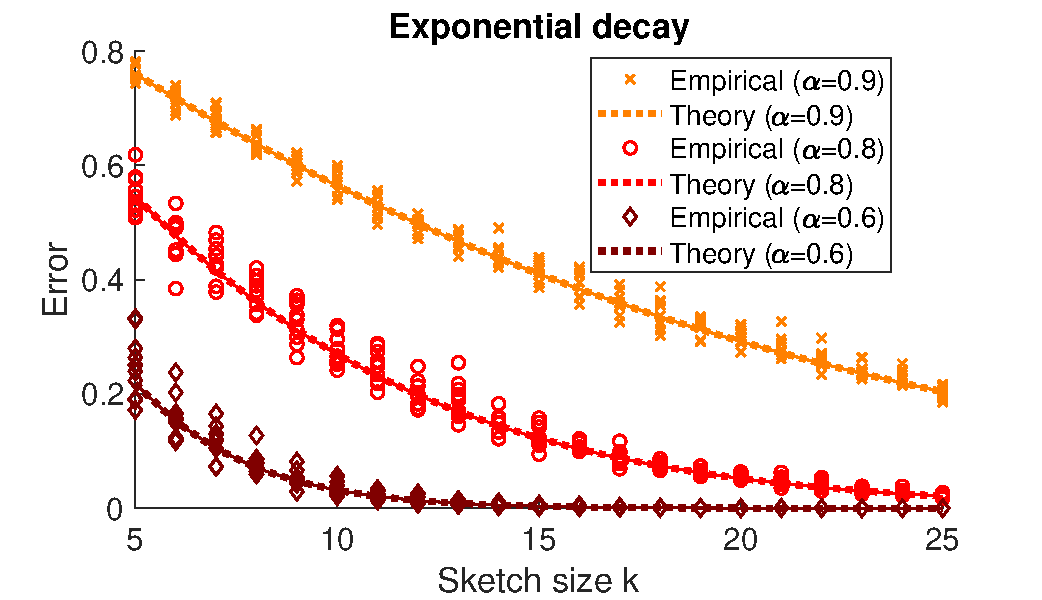
\includegraphics[width=\textwidth]{explicit_exp}
    \end{subfigure}
\hfill
    \begin{subfigure}{0.49\textwidth}%
\subcaption{Singular values are given by $\sigma_i^2=C\cdot i^{-\beta}$.}
      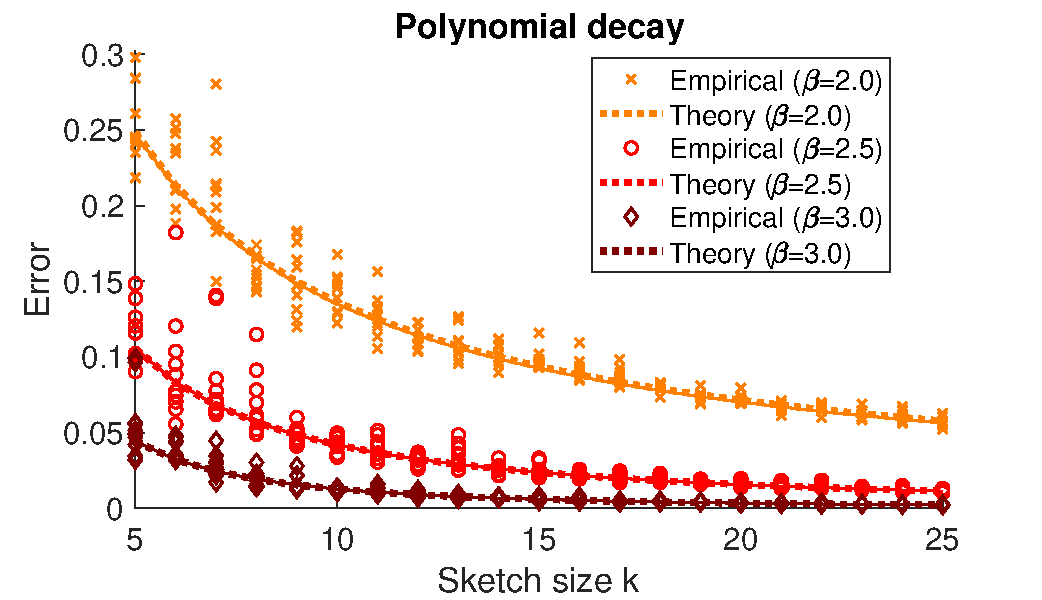
\includegraphics[width=\textwidth]{explicit_poly}
    \end{subfigure}
\caption{
Theoretical predictions of low-rank approximation error of a Gaussian
sketch under known spectral decays, compared to the empirical results.
The constant $C$ is scaled so that $\|\A\|_F^2=1$ and we let
$n=m=1000$. For the theory, we plot the explicit formulas
\eqref{eq:explicit-exp} and \eqref{eq:explicit-poly} (dashed lines),
as well as the implicit expression from Corollary \ref{c:low-rank}
(thin solid lines) obtained by numerically solving
\eqref{eq:equation}. Observe that the explicit and implicit
predictions are nearly (but not exactly) identical.
}
%\vspace{-5mm}
\label{f:explicit}
\end{figure}


\subsection{Exponential spectral decay}
Suppose that the squared singular values of $\A$ exhibit exponential
decay, i.e. $\sigma_i^2 = C\cdot \alpha^{i-1}$, where $C$ is a constant
and $\alpha\in(0,1)$. For simplicity of presentation, we will let
$m,n\rightarrow\infty$. Under this spectral decay, we can approximate
the sum in \eqref{eq:equation} by the analytically computable integral
$\int_y^\infty\!\frac1{1+(C\gamma)^{-1}\alpha^{-x}} dx$,
% \begin{align*}
%   \underbrace{\int_{0}^\infty\frac1{1+(C\gamma)^{-1}\alpha^{-x}}
%   dx}_{\frac{\ln(1/(C\gamma+1))}{\ln(\alpha)}}\ \leq\ 
%   \underbrace{\sum_{i\geq
%   1}\frac{\gamma\sigma_i^2}{\gamma\sigma_i^2+1}}_{k}
%  \ \leq\
%   \underbrace{\int_{-1}^\infty\frac1{1+(C\gamma)^{-1}\alpha^{-x}}
%   dx}_{\frac{\ln(\alpha/(C\gamma+\alpha))}{\ln(\alpha)}}.
% % =\frac1{2\ln(\alpha)}\bigg(\ln\Big(\frac{\alpha}{C\gamma+\alpha}\Big)
% %     +\ln\Big(\frac{1}{C\gamma+1}\Big)\bigg). 
% % 
%   \end{align*}
% Using each integral as a proxy for the sum, solving for $\gamma$, and
% taking a geometric mean of the two results,
obtaining $\gamma\approx(\alpha^{-k}-1)\sqrt\alpha/C$. Applying this to the
formula from Corollary~\ref{c:low-rank}, we can express the low-rank
approximation error  
for a sketch of size $k$ as follows:
\begin{align}
  \E\big[\|\A-\A\P\|_F^2\big] \approx
\frac C{\sqrt\alpha}\cdot
  \frac{k}{\alpha^{-k}-1},\quad\text{when}\quad\sigma_i^2=C\cdot\alpha^{i-1}\
  \ \text{for all $i$.}\label{eq:explicit-exp}
\end{align}
In Figure \ref{f:explicit}a, we plot the above formula against the
numerically obtained implicit expression from
Corollary~\ref{c:low-rank}, as well as empirical results for a Gaussian 
sketch. First, we observe that the theoretical predictions closely
align with empirical values even after the sketch size crosses the
stable rank $r\approx\frac1{1-\alpha}$, suggesting that Theorem \ref{t:main} can
be extended to this regime. Second, while it is not surprising that
the error decays at a similar 
rate as the singular values, our predictions offer a much more precise
description, down to lower order effects and
even constant factors. For instance, we observe that the error
(normalized by $\|\A\|_F^2$, as in the figure) only
starts decaying exponentially after $k$ crosses the stable rank, and
until that point it decreases at a linear rate with slope
$-\frac{1-\alpha}{2\sqrt\alpha}$.

 

\subsection{Polynomial spectral decay}
We now turn to polynomial spectral decay, which is a natural model for
analyzing heavy-tailed data distributions. Let $\A$ have squared
singular values $\sigma_i^2=C\cdot i^{-\beta}$ for some $\beta\geq 2$, and let
$m,n\rightarrow\infty$. As in the case of exponential decay,
we use the integral $\int_y^\infty\!\frac1{1+(C\gamma)^{-1}x^{-\beta}}dx$
to approximate the sum in \eqref{eq:equation}, and 
solve for $\gamma$, obtaining $\gamma \approx
\big((k+\frac12)\frac\beta\pi\sin(\frac\pi\beta)\big)^\beta$. Combining
this with Corollary \ref{c:low-rank} we get:
\begin{align}
  \E\big[\|\A-\A\P\|_F^2\big] \approx
  C\cdot\frac{k}{(k+\frac12)^\beta}\bigg(\frac{\pi/\beta}{\sin(\pi/\beta)}\bigg)^\beta,
  \quad\text{when}\quad\sigma_i^2=C\cdot
  i^{-\beta}\ \ \text{for all $i$.}\label{eq:explicit-poly}
\end{align}

Figure \ref{f:explicit}b compares our predictions to the empirical
results for several values of $\beta$. In all of these cases, the
stable rank is close to 1, and yet the theoretical predictions align
very well with the empirical results. Overall, the asymptotic rate of decay of the error is
$k^{1-\beta}$.  However it is easy to verify that the lower order
effect of $(k+\frac12)^\beta$ appearing instead of $k^\beta$
in \eqref{eq:explicit-poly} significantly changes the trajectory for
small values of $k$. Also, note that as $\beta$ grows large, the
constant $\big(\frac{\pi/\beta}{\sin(\pi/\beta)}\big)^\beta$ goes to
$1$, but it plays a significant role for $\beta=2$ or $3$
(roughly, scaling the expression by a factor of $2$). Finally, we
remark that for $\beta\in(1,2)$, our integral approximation of
\eqref{eq:equation} becomes less accurate. We expect that a corrected
expression is possible, but likely more complicated and less interpretable.
\vspace{3mm}


\ifisarxiv
\else
\begin{minipage}{.48\textwidth}
\hspace{-4.5mm}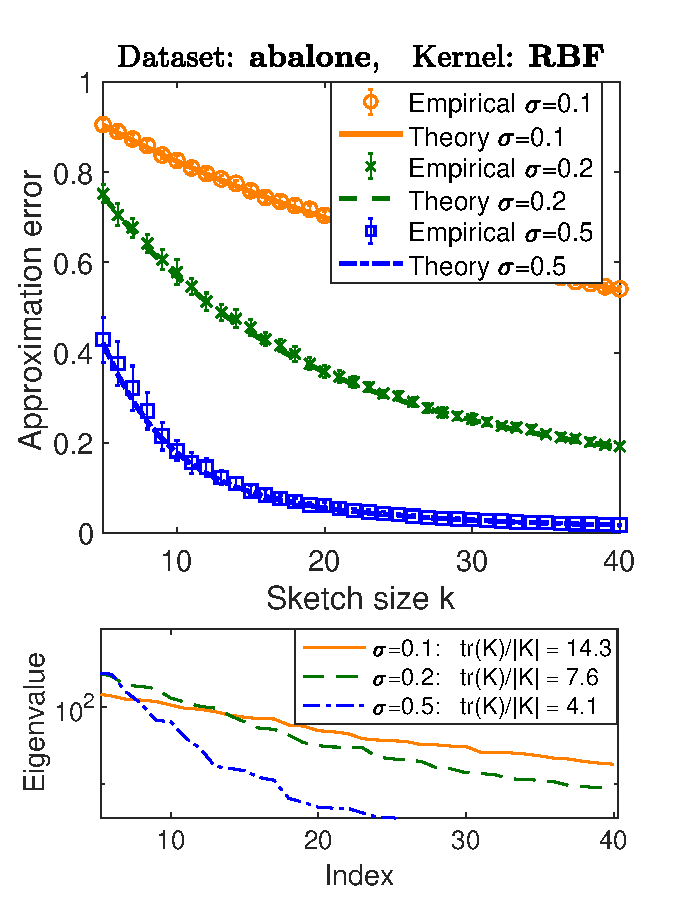
\includegraphics[width=.57\textwidth]{abalone-nystrom}\nobreak\hspace{-2.5mm}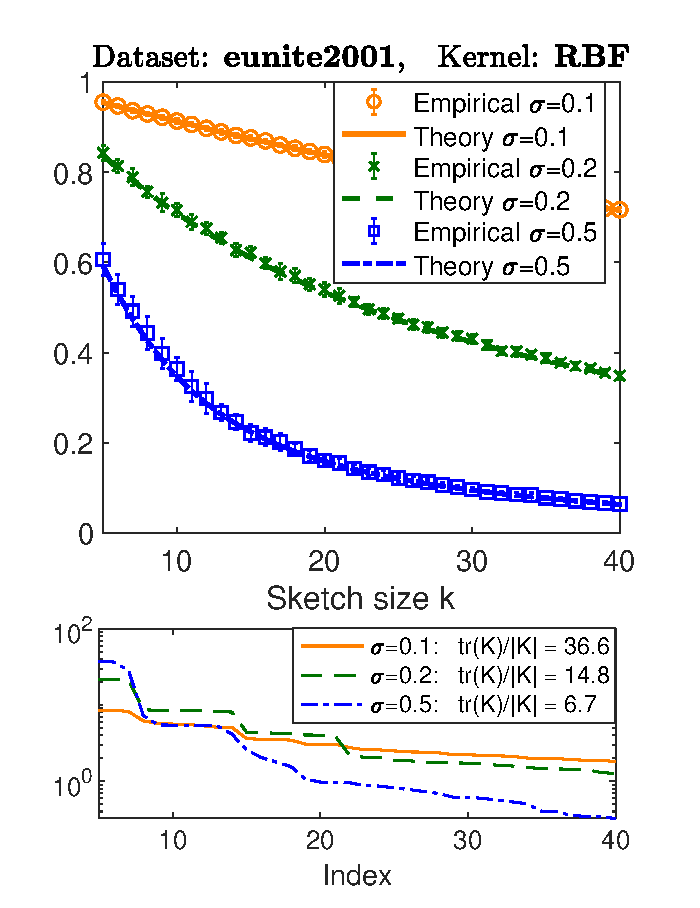
\includegraphics[width=.57\textwidth]{eunite-nystrom}\vspace{-1mm}
  \captionof{figure}{Theoretical predictions versus approximation error for the
    sketched Nystr\"om with the RBF kernel
    (spectral decay shown at the bottom).}\label{f:nystrom}
\end{minipage}\hspace{4mm}
\begin{minipage}{.48\textwidth}
\hspace{-2.5mm}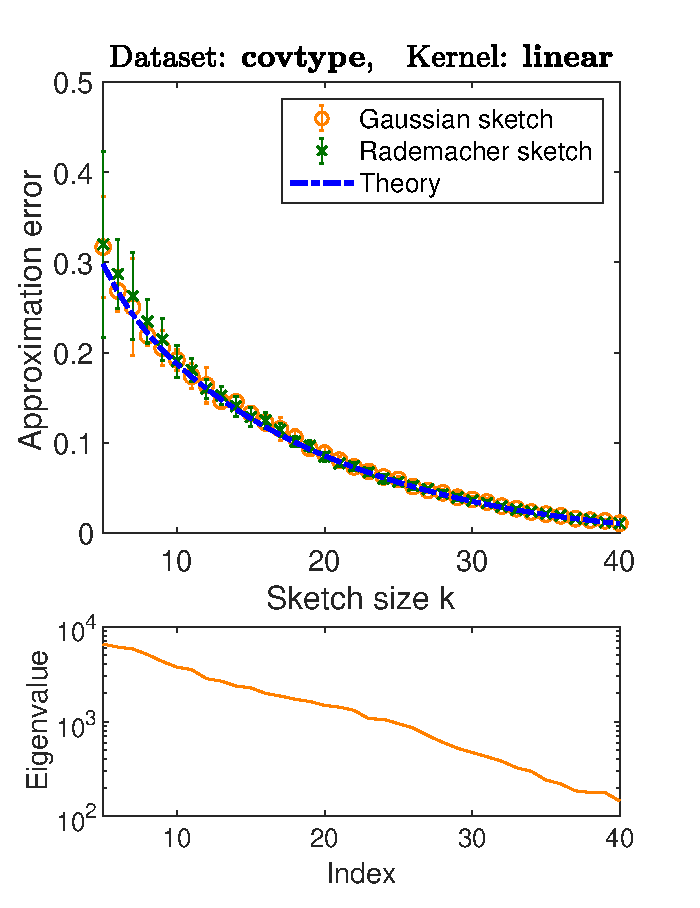
\includegraphics[width=.57\textwidth]{covtype-linear}\nobreak\hspace{-2.5mm}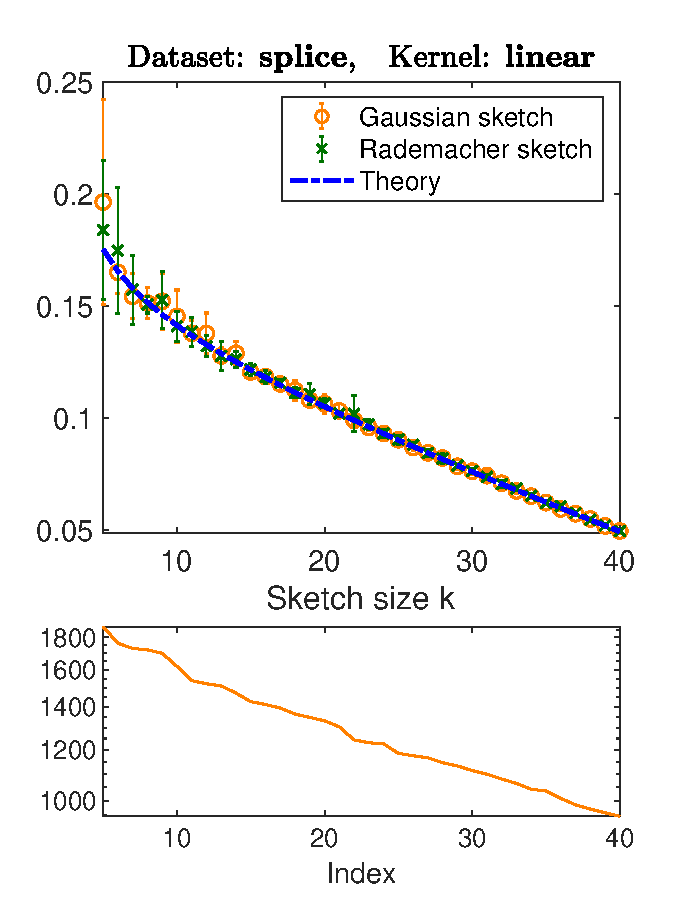
\includegraphics[width=.57\textwidth]{splice-linear}\vspace{-1mm}
  \captionof{figure}{Theoretical predictions versus approximation error for
the Gaussian and Rademacher sketches
  (spectral decay shown at the bottom).}\label{f:linear}
\end{minipage}
\fi

\section{Empirical results}\label{s:experiments}

In this section, we numerically verify the accuracy of our theoretical
predictions for the low-rank approximation error of sketching on
benchmark datasets from the libsvm repository 
\cite{libsvm} (further numerical results are in
Appendix~\ref{a:experiments}). We repeated every experiment 10 times,
and plot 
both the average and standard deviation of the results. We use the
following $k\times m$ sketching matrices $\S$:\vspace{-1mm}
\begin{enumerate}
\item \emph{Gaussian sketch:} with i.i.d.\@ standard normal entries;
\item \emph{Rademacher sketch:} with
  i.i.d.\@ entries equal $1$ with probability 0.5 and $-1$ otherwise.
\end{enumerate}
\vspace{-2mm}

\ifisarxiv
\begin{figure}
  \centering
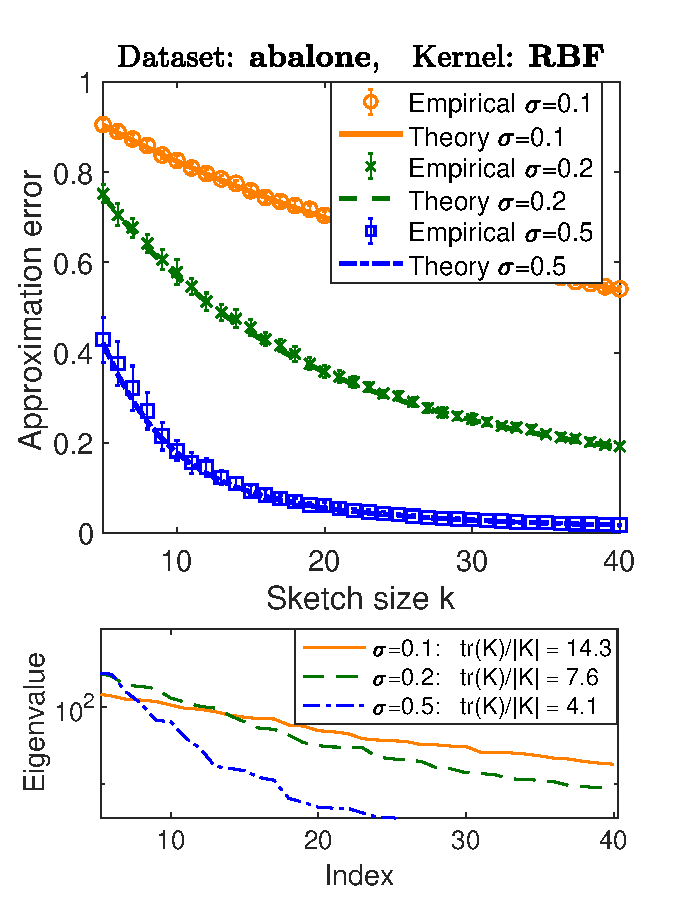
\includegraphics[width=.43\textwidth]{abalone-nystrom}\nobreak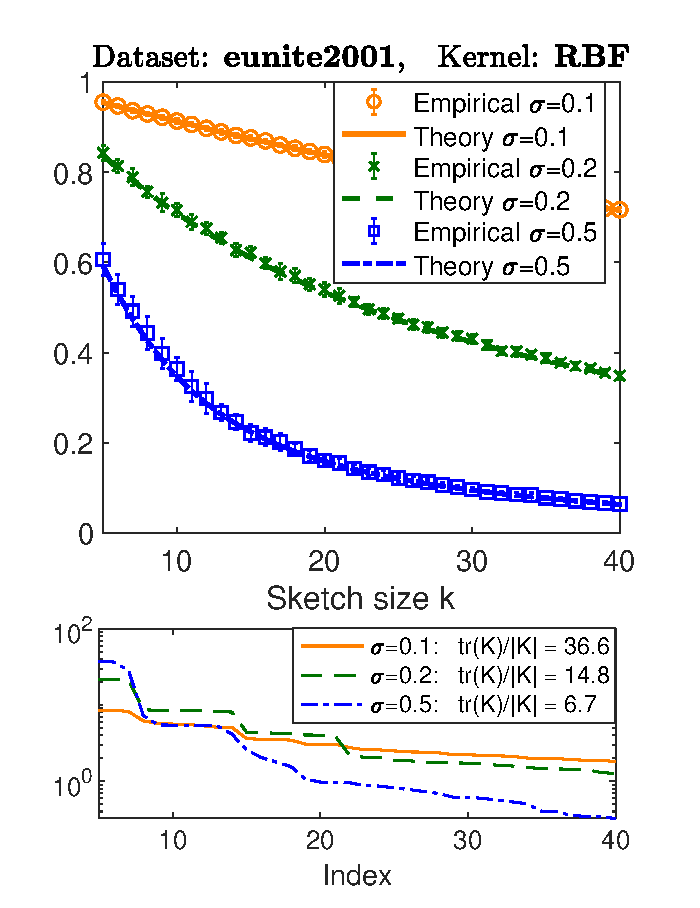
\includegraphics[width=.43\textwidth]{eunite-nystrom}
  \caption{Theoretical predictions versus approximation error for the
    sketched Nystr\"om with the RBF kernel
    (spectral decay shown at the bottom).}\label{f:nystrom}
\end{figure}
\fi

\ifisarxiv
\begin{figure}
  \centering
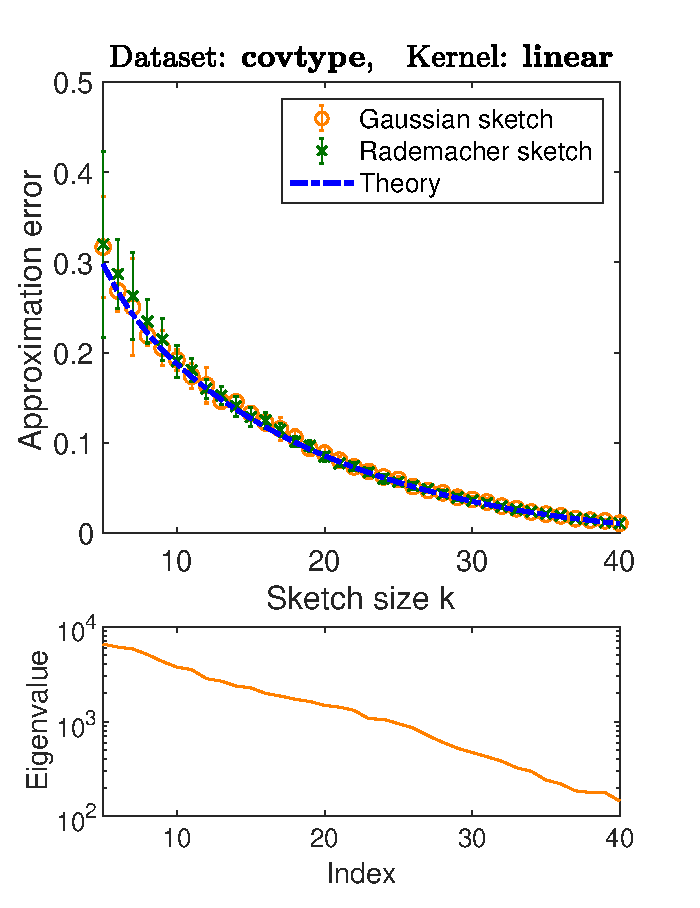
\includegraphics[width=.43\textwidth]{covtype-linear}\nobreak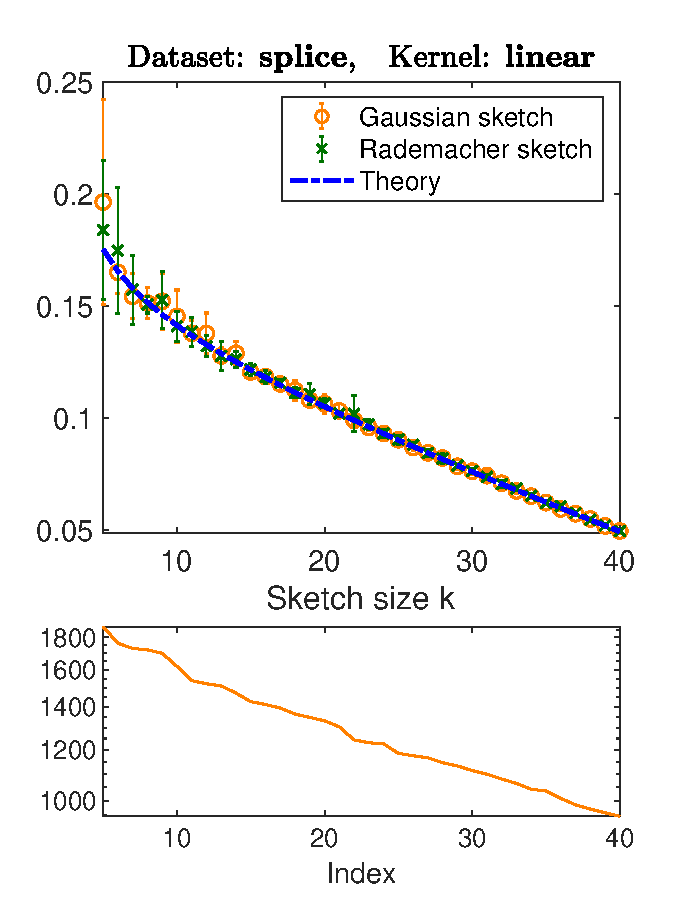
\includegraphics[width=.43\textwidth]{splice-linear}
  \caption{Theoretical predictions versus approximation error for
the Gaussian and Rademacher sketches
  (spectral decay shown at the bottom).}\label{f:linear}
\end{figure}
\fi

\paragraph{Varying spectral decay.}  To demonstrate the role of spectral
decay and the stable rank on the approximation error, we performed
feature expansion using the radial basis function (RBF) kernel
$k(\a_i,\a_j)=\exp(-\|\a_i-\a_j\|^2/(2\sigma^2))$, obtaining an $m\times m$
kernel matrix $\K$. We used the sketched Nystr\"om method to construct
a low-rank approximation $\tilde
\K=\K\S^\top(\S\K\S^\top)^\dagger\S\K$, and computed the normalized trace norm 
error $\|\K-\tilde\K\|_*/\|\K\|_*$. The theoretical predictions are coming from
\eqref{eq:nystrom}, which in turn uses Theorem \ref{t:main}.
% The scale parameter
% $\sigma>0$ significantly affects the spectral properties of the kernel,
% so varying it allows us to observe qualitatively different behavior of
% the approximation error. Note that t
% The choice of $\sigma$ used in
% practice depends on the down-stream task, and is often determined by
% cross-validation.
Following \cite{revisiting-nystrom}, we use the RBF kernel because
varying the scale parameter $\sigma$ 
allows us to observe the approximation error under qualitatively
different spectral decay profiles of the kernel. In Figure \ref{f:nystrom},
we present the results for the Gaussian sketch on two datasets, with three values
of $\sigma$, and in all cases our theory aligns with the empirical
results. Furthermore, as smaller $\sigma$ leads to slower spectral decay and 
larger stable rank, it also makes the approximation error decay more
linearly for small sketch sizes. This behavior is predicted by our explicit
expressions \eqref{eq:explicit-exp} for the error under exponential spectral decay from
Section \ref{s:explicit}. Once the sketch sizes are sufficiently
larger than the stable rank of $\K^{\frac12}$, the error starts decaying at an
exponential rate. Note that Theorem \ref{t:main} only guarantees
accuracy of our expressions for sketch sizes below the stable rank,
however the predictions are accurate regardless of this constraint.
\vspace{-2mm}
\paragraph{Varying sketch type.} In the next set of
empirical results, we compare the performance of Gaussian and Rademacher
sketches, and also verify the theory when sketching the data matrix $\A$
without kernel expansion, plotting
$\|\A-\A(\S\A)^\dagger\S\A\|_F^2/\|\A\|_F^2$.
Since both of the sketching methods have 
sub-gaussian entries, Corollary~\ref{c:low-rank} predicts that they
should have comparable performance in this task and match our
expressions. This is exactly what we observe in Figure \ref{f:linear}
for two datasets and a range of sketching sizes, as well as in other
empirical results shown in Appendix \ref{a:experiments}.

\section{Conclusions}

We derived the first theoretically supported precise expressions for the
expected residual projection matrix, which is a central component in
the analysis of RandNLA dimensionality reduction via sketching. Our
analysis provides a new understanding of low-rank approximation, the Nystr\"om method, and the
convergence properties of many randomized iterative algorithms. As a direction for future work, we conjecture that our
main result can be extended to sketch sizes larger than the stable
rank of the data matrix.

\ifisarxiv\else
\section*{Broader Impact}
In this paper, we investigate the spectral properties of residual
(random) projection matrices, commonly appearing in various
sketching-based methods. The precise theoretical description given in
this paper provides performance guarantees for popular algorithms
such as low-rank approximation and many randomized (iterative)
optimization methods, and contributes to the development of more
robust and reliable large-scale learning systems. The
theoretical framework developed in this work presents no foreseeable
negative societal consequence. 
\fi


\paragraph{Acknowledgments.}
We would like to acknowledge DARPA, NSF, and ONR for providing partial support of this work.


% \bibliographystyle{alpha}
% \bibliography{../pap}


% In this section, we report experimental evidence illustrating our results
% provide meaningful approximations on a variety of conditions and real-world
% datasets.

% In \Cref{f:main} we use synthetic data to investigate the size of the error
% ($\epsilon$) as well as its rate of decay. $\A$ is taken to be diagonal with
% eigenvalues decaying exponentially from $1$ to $0.1$. As a result, we are both
% able to let $r$ grow arbitrarily large as well as choose a sketch size $k$ such
% that the aspect ratio $\rho$ remains constant. As the constants hidden
% in $O(1/\sqrt{r})$ depend on $\rho$, such a scaling enables isolation
% of the relation between approximation quality $\epsilon$ and stable rank $r$.
% We construct bootstrapped operator norm confidence intervals using
% \cite{lopes2019bootstrapping}.

% \begin{figure}[htbp]
%   \centering
%   \includegraphics[width=1.0\linewidth]{../equivalents_code/theorem1.png}
%   \caption{Visualization of the $\epsilon$ in \Cref{t:main} for two different
%     sub-gaussian sketching matrices $\mathbf{S}$.
%   }
%   \label{f:main}
% \end{figure}

% The results in \Cref{f:main} show that the approximation quality becomes
% small relatively quickly, and that the reciprocal-like rate of decay holds
% both across a range of aspect ratios $\rho$ as well as over different
% sub-gaussian sketching matrices $\S$.

% Beyond synthetic data, we interrogate the practical applicability of our
% results by performing experiments on real-world datasets to empirically verify
% that \Cref{c:low-rank} provides useful predictions. We chose to present
% datasets representing a diversity of conditions here
% (see \Cref{tab:datasets}), though we conducted a more extensive investigation
% and report full results in Appendix \todo{feynman}.

% \begin{table}[htpb]
%   \centering
%   \caption{Summary statistics for \texttt{libsvm} \citep{libsvm} datasets used}
%   \label{tab:datasets}
%   \begin{tabular}{ccccc}
%     \toprule
%     Name & Rows ($n$) & Columns ($d$) & Rows / Columns & Stable rank ($r$) \\
%     \midrule
%     %abalone\_scale & 4177 & 8 & 5.2e+02 & 1.57 \\
%     %housing\_scale & 506 & 13 & 39 & 1.75 \\
%     %mg\_scale & 1385 & 6 & 2.3e+02 & 2.32 \\
%     %mpg\_scale & 392 & 7 & 56 & 1.85 \\
%     %pyrim\_scale & 74 & 27 & 2.7 & 1.50 \\
%     %triazines\_scale & 186 & 60 & 3.1 & 1.40 \\
%     cpusmall\_scale & 8192 & 12 & \textbf{6.8e+02} & 1.06 \\
%     bodyfat\_scale & 252 & 14 & 18 & 1.32 \\
%     splice\_scale & 1000 & 60 & 17 & \textbf{18.65} \\
%     real-sim & 72309 & \textbf{20958} & 3.45 & 7.46 \\
%     cifar10 & 50000 & 3072 & 16.28 & 1.15 \\
%     SVHN & \textbf{73257} & 3072 & 23.85 & 1.06 \\
%     \bottomrule
%   \end{tabular}
% \end{table}

% % \begin{figure}[htbp]
% %   \centering
% %   \includegraphics[width=1.0\linewidth]{../equivalents_code/corollary1.png}
% %   \caption{
% %     \Cref{c:low-rank} approximations of the reconstruction error (blue) 
% %     closely follows the mean across many real-world datasets.
% %   }
% %   \label{f:low-rank}
% % \end{figure}

% In \Cref{f:low-rank}, we display the predicted reconstruction error using our
% theory as well as a box plot summarizing the empirical distribution of samples
% of $\|\A - \A\P\|_F^2$. Notice that our theoretical predictions are very
% close to the empirical means even for extremely small sketch sizes, and
% that the results are applicable on datasets as small as
% $252 \times 14$ (bodyfat\_scale) to as large as $72309 \times 20958$
% (real-sim). As expected, cifar10 and SVHN results appear similar because
% they are both image datasets with the same number of dimensions
% and similar stable ranks.
% Also, when the stable rank is large (splice\_scale and real-sim)
% we see that both the empirical and predicted reconstruction errors decay
% at a significantly slower rate than when it is small. This further supports
% the view that stable rank is the ``correct'' notion to consider in the context
% of low rank approximation.



% \appendix
% 


\section{Proof of Lemma~\ref{l:size}}
\label{appx: proof-of-l-size}

We first record an important property of the design $S_\mu^d$
which can be used to construct an over-determined design for any $n>d$. A similar
version of this result was also previously shown by
\cite{correcting-bias-journal} for a different determinantal design.

\begin{lemma}\label{l:decomposition}
  Let $\Xb\sim S_\mu^d$ and $\X\sim \mu^K$, where
  $K\sim\Poisson(\gamma)$. Then the matrix composed of a random
  permutation of the rows from $\Xb$ and $\X$ is distributed according to
  $S_\mu^{d+\gamma}$.
\end{lemma}

\begin{proof}
Let $\Xt$ denote the matrix constructed from the permuted rows of
$\Xb$ and $\X$.  Letting $\Z\sim\mu^{K+d}$, we derive the probability
$\Pr\big\{\Xt\!\in\! E\big\}$ by summing over the possible index subsets  $S\subseteq
[K+d]$ that correspond to the rows coming from $\Xb$:
\begin{align*}
  \Pr\big\{\Xt\in E\big\} &= \E\bigg[\frac{1}{\binom{K+d}{d}}
  \sum_{S:\,|S|=d}\frac{\E[\det(\Z_{S,*})^2\one_{[\Z\in E]}\mid
  K]}{d!\det(\Sigmab_\mu)}\bigg]\\
  &=\sum_{k=0}^\infty
    \frac{\gamma^k\ee^{-\gamma}}{k!}\,\frac{\gamma^dk!}{(k+d)!}\,
    \frac{\E\big[\sum_{S:\,|S|=d}\det(\Z_{S,*})^2\one_{[\Z\in E]}\mid
    K=k\big]}{\det(\gamma\Sigmab_\mu)}\\
  &\overset{(*)}{=} \sum_{k=0}^\infty
    \frac{\gamma^{k+d}\ee^{-\gamma}}{(k+d)!}
    \,\frac{\E[\det(\Z^\top\Z)\one_{[\Z\in E]}\mid K=k]}{\det(\gamma\Sigmab_\mu)},
\end{align*}
where $(*)$ uses the Cauchy-Binet formula to sum over all subsets $S$
of size $d$. Finally, since the sum shifts from $k$
to $k+d$, the last expression can be rewritten as
$\E[\det(\X^\top\X)\one_{[\X\in E]}]/\det(\gamma\Sigmab_\mu)$, where recall that
$\X\sim\mu^K$ and $K\sim\Poisson(\gamma)$, matching the definition of $S_\mu^{d+\gamma}$.
\end{proof}

We now proceed with the proof of Lemma \ref{l:size}, where we establish
that the expected sample size of $S_\mu^n$ is indeed $n$.

\begin{proofof}{Lemma}{\ref{l:size}}
  The result is obvious when $n=d$, whereas
  for $n>d$ it is an immediate consequence
  of Lemma \ref{l:decomposition}.
  Finally, for $n<d$ the expected sample
  size follows as a corollary of Lemma \ref{l:proj}, which states that
  \begin{align*}
\text{(Lemma \ref{l:proj})} \qquad\E\big[\I - \Xb^\dagger\Xb\big] =
    (\gamma_n\Sigmab_\mu + \I)^{-1},
  \end{align*}
  where $\Xb^\dagger\Xb$ is the orthogonal projection onto
  the subspace spanned by the rows of $\Xb$. Since the rank of this
  subspace is equal to the number of the rows, we have
  $\#(\Xb)=\tr(\Xb^\dagger\Xb)$, so
  \begin{align*}
    \E\big[\#(\Xb)\big] = d - \tr\big((\gamma_n\Sigmab_\mu +
    \I)^{-1}\big) =
    \tr\big(\gamma_n\Sigmab_\mu(\gamma_n\Sigmab_\mu+\I)^{-1}\big) = n,
  \end{align*}
  which completes the proof.
\end{proofof}

\section{Proofs for Section \ref{s:dp}}
\label{a:dp}

We use $\adj(\A)$ to denote the adjugate of $\A$, defined as follows: the
$(i,j)$th entry of $\adj(\A)$ is
$(-1)^{i+j}\det(\A_{[n]\backslash\{j\},[n]\backslash\{i\}})$.
We will use two useful identities related to the adjugate: (1)
$\adj(\A)=\det(\A)\A^{-1}$ for invertible $\A$, and (2)
$\det(\A+\u\v^\top)=\det(\A)+\v^\top\!\adj(\A)\u$
\citep[see Fact 2.14.2 in][]{matrix-mathematics}.

First, note that from the definition of an adjugate matrix it immediately follows that if $\A$ is
determinant preserving then adjugate commutes with expectation for this matrix:
\begin{align}
  \E\big[\big(\!\adj(\A)\big)_{i,j}\big] &=
  \E\big[(-1)^{i+j}\det(\A_{[d]\backslash\{j\},[d]\backslash\{i\}})\big]\nonumber
  \\
&=(-1)^{i+j}\det\!\big(\E[\A_{[d]\backslash\{j\},[d]\backslash\{i\}}]\big)
  \\
  &= \big(\!\adj(\E[\A])\big)_{i,j}.\label{eq:adj}
\end{align}
% The adjugate is useful in our analysis because it connects the
% determinant and the inverse via the formula
% $\adj(\A)=\det(\A)\A^{-1}$, which holds for any invertible $\A$.


\begin{proofof}{Lemma}{\ref{t:ring}} \
 First, we show that $\A+\u\v^\top$ is d.p.~for any fixed
 $\u,\v\in\R^d$. Below, we use the identity for a rank one
 update of a determinant:
 $\det(\A+\u\v^\top)=\det(\A)+\v^\top\!\adj(\A)\u$. It follows that
 for any $\Ic$ and $\Jc$ of the same size,
  \begin{align*}
\E\big[\!\det(\A_{\Ic,\Jc}\!+\u_{\Ic}\v_{\Jc}^\top)\big] &=
    \E\big[\!\det(\A_{\Ic,\Jc}) +
    \v_{\Jc}^\top\adj(\A_{\Ic,\Jc}) \u_{\Ic}\big]\\
    &\overset{(*)}{=}\det\!\big(\E[\A_{\Ic,\Jc}]\big) +
      \v_{\Jc}^\top\adj\!\big(\E[\A_{\Ic,\Jc}]\big) \u_{\Ic}\\
    &=\det\!\big(\E[\A_{\Ic,\Jc} \!+ \u_{\Ic}\v_{\Jc}^\top]\big),
  \end{align*}
  where $(*)$ used \eqref{eq:adj}, i.e., the fact that for d.p.~matrices, adjugate commutes
  with expectation. Crucially, through the definition of an adjugate
  this step implicitly relies on the assumption that all the square
  submatrices of $\A_{\Ic,\Jc}$ are also  determinant preserving.
  Iterating this, we get that $\A+\Z$ is d.p.~for any fixed
  $\Z$. We now show the same for $\A+\B$:
  \begin{align*}
\E\big[\!\det(\A_{\Ic,\Jc}\!+\B_{\Ic,\Jc})\big]
    &=
      \E\Big[\E\big[\!\det(\A_{\Ic,\Jc}\!+\B_{\Ic,\Jc})\mid\B\big]\Big]\\
    &\overset{(*)}{=}\E\Big[\!\det\!\big(\E[\A_{\Ic,\Jc}]\!+\B_{\Ic,\Jc}\big)\Big]\\
      &= \det\!\big(\E[\A_{\Ic,\Jc}\!+\B_{\Ic,\Jc}]\big),
  \end{align*}
  where $(*)$  uses the fact that after conditioning on $\B$ we can
  treat it as a fixed matrix. Next, we show that $\A\B$ is determinant preserving via the Cauchy-Binet formula:
  \begin{align*}
    \E\big[\!\det\!\big((\A\B)_{\Ic,\Jc}\big)\big]
    &= \E\big[\!\det(\A_{\Ic,*}\B_{*,\Jc})\big]\\
    &=\E\bigg[\sum_{S:\,|S|=|\Ic|}\!\!\det\!\big(\A_{\Ic,S}\big)
      \det\!\big(\B_{S,\Jc}\big)\bigg]\\
&=\!\!\sum_{S:\,|S|=|\Ic|}\!\!\det\!\big(\E[\A]_{\Ic,S}\big)
                                                \det\!\big(\E[\B]_{S,\Jc}\big)\\
    &=\det\!\big(\E[\A]_{\Ic,*}\, \E[\B]_{*,\Jc}\big)\\
      &= \det\!\big(\E[\A\B]_{\Ic,\Jc}\big),
  \end{align*}
  where recall that $\A_{\Ic,*}$ denotes the submatrix of $\A$
  consisting of its (entire) rows indexed by $\Ic$.
  \end{proofof}

To prove Lemma \ref{l:poisson}, we will use the following
lemma, many variants of which appeared in the literature
\cite[e.g.,][]{expected-generalized-variance}. We use the one given by
\cite{correcting-bias}.
\begin{lemma}[\cite{correcting-bias}]\label{l:cb}
If the rows of random $k\times d$ matrices $\A,\B$
  are sampled as an i.i.d.~sequence of $k\geq d$ pairs of joint random vectors, then
\begin{align}
  k^d\,\E \big[\det(\A^\top\B)\big]
  &= \ktd\,\det\!\big(\E[\A^\top\B]\big).
     \end{align}
 \end{lemma}

\noindent
Here, we use the following standard shorthand: $\ktd =
\frac{k!}{(k-d)!} = k\,(k-1)\dotsm(k-d+1)$. Note that the above result
almost looks like we are claiming that the matrix $\A^\top\B$ is d.p.,
but in fact it is not because $k^d\neq \ktd$. The difference
in those factors is precisely what we are going to correct with the
Poisson random variable. We now present the proof of Lemma
\ref{l:poisson}.
\begin{proofof}{Lemma}{\ref{l:poisson}}
Without loss of generality, it suffices to check Definition \ref{d:main} with both $\Ic$ and
$\Jc$ equal $[d]$. We first expand the expectation by
conditioning on the value of $K$ and letting $\gamma=\E[K]$:
    \begin{align*}
      \E\big[\!\det(\A^\top\B)\big]
      &= \sum_{k=0}^\infty
\E\big[\det(\A^\top\B)\mid K\!=\!k\big]\
\Pr(K\!=\!k)\\
      \text{(Lemma \ref{l:cb})}
      \quad&=
        \sum_{k=d}^\infty\frac{k! k^{-d}}{(k-d)!}\det\!\big(\E[\A^\top\B\mid
        K\!=\!k]\big)
        \frac{\gamma^k\ee^{-\gamma}}{k!}\\
      &=\sum_{k=d}^\infty
\Big(\frac\gamma k\Big)^d\det\!\big(\E[\A^\top\B\mid K\!=\!k]\big)
        \frac{\gamma^{k-d}\ee^{-\gamma}}{(k-d)!}.
     %  \\
     %  &=\sum_{k=0}^\infty \det\!\big(\E[\A^\top\B]\big)\,\Pr(K\!=\!k)
     % \ =\ \det\!\big(\E[\A^\top\B]\big).
    \end{align*}
    Note that $\frac\gamma k\,\E[\A^\top\B\mid K\!=\!k]=\E[\A^\top\B]$,
    which is independent of $k$. Thus we can rewrite the above
    expression as:
    \begin{align*}
\det\!\big(\E[\A^\top\B]\big)\sum_{k=d}^\infty\frac{\gamma^{k-d}\ee^{-\gamma}}{(k-d)!}
      =
      \det\!\big(\E[\A^\top\B]\big)\sum_{k=0}^\infty
      \frac{\gamma^{k}\ee^{-\gamma}}{k!}=\det\!\big(\E[\A^\top\B]\big),
    \end{align*}
    which concludes the proof.
  \end{proofof}

To prove Lemma \ref{l:normalization}, we use the following standard
determinantal formula which is used to derive the normalization
constant of a discrete determinantal point process.
\begin{lemma}[\cite{dpp-ml}]\label{l:det-standard}
  For any $k\times d$ matrices $\A,\B$ we have
  \[\det(\I+\A\B^\top)=\sum_{S\subseteq[k]}\det(\A_{S,*}\B_{S,*}^\top).\]
\end{lemma}

\begin{proofof}{Lemma}{\ref{l:normalization}}
By Lemma \ref{l:poisson}, the matrix $\B^\top\A$ is determinant
preserving. Applying Lemma \ref{t:ring} we conclude that
$\I+\B^\top\A$ is also d.p., so
\begin{align*}
  \det\!\big(\I+\E[\B^\top\A]\big) = \E\big[\det(\I+\B^\top\A)\big] =\E\big[\det(\I+\A\B^\top)\big],
\end{align*}
where the second equality is known as Sylvester's Theorem.
We rewrite the expectation of $\det(\I+\A\B^\top)$ by applying Lemma
\ref{l:det-standard}.  Letting $\gamma=\E[K]$, we obtain:
\begin{align*}
\E\big[\det(\I+\A\B^\top)\big]  &=\E\bigg[\sum_{S\subseteq [K]}\E\big[\det(\A_{S,*}\B_{S,*}^\top)\mid
    K\big]\bigg]\\
  &\overset{(*)}{=}\sum_{k=0}^\infty\frac{\gamma^k\ee^{-\gamma}}{k!}
  \sum_{i=0}^k\binom{k}{i} \E\big[\det(\A\B^\top)\mid K=i\big]\\
  &=\sum_{i=0}^\infty \E\big[\det(\A\B^\top)\mid K=i\big]
  \sum_{k\geq i}^\infty \binom{k}{i}
  \frac{\gamma^k\ee^{-\gamma}}{k!}\\
  &=\sum_{i=0}^\infty
    \frac{\gamma^i\ee^{-\gamma}}{i!}\E\big[\det(\A\B^\top)\mid K=i\big]
    \sum_{k\geq i}^\infty\frac{\gamma^{k-i}}{(k-i)!} = \E\big[\det(\A\B^\top)\big]\cdot\ee^\gamma,
\end{align*}
where $(*)$ follows from the exchangeability of the rows of $\A$ and
$\B$, which implies that the distribution of $\A_{S,*}\B_{S,*}^\top$ is the
same for all subsets $S$ of a fixed size $k$.
\end{proofof}

\section{Proof of Theorem \ref{t:mse}}
\label{a:mse-proof}
In this section we use $Z_\mu^n$ to denote the normalization
constant that appears in \eqref{eq:cases} when computing an expectation for surrogate design
$S_\mu^n$.
We first prove Lemma \ref{l:sqinv-all}. % by splitting the under- and
% over-determined cases and start with proving the former.
% Note that those
% results require $\mu$ to satisfy general position (Assumption \ref{a:general-position}),
% which implies that if $\X\sim\mu^k$ for $k\leq d$ then $\rank(\X)=k$.
\begin{lemma}[restated Lemma \ref{l:sqinv-all}]\label{l:sqinv-under}
If  $\Xb\sim S_\mu^n$ for $n<d$, then we have
\begin{align*}
    \E\big[\tr\big((\Xb^\top\Xb)^{\dagger}\big)\big]
    &={\gamma_n}\big(1- \det\!\big((\tfrac1{\gamma_n}\I+\Sigmab_\mu)^{-1}\Sigmab_\mu\big)\big).
\end{align*}
\end{lemma}
\begin{proof}
Let $\X\sim\mu^K$ for $K\sim\Poisson({\gamma_n})$. Note that if
$\det(\X\X^\top)>0$ then using the fact that
$\det(\A)\A^{-1}=\adj(\A)$ for any invertible matrix $\A$, we can write:
  \begin{align*}
    \det(\X\X^\top)\tr\big((\X^\top\X)^{\dagger}\big)
    &= \det(\X\X^\top)\tr\big((\X\X^\top)^{-1}\big) \\
    &= \tr(\adj(\X\X^\top)) \\[-1mm]
    &= \sum_{i=1}^K\det(\X_{-i}\X_{-i}^\top),
  \end{align*}
  where $\X_{-i}$ is a shorthand for $\X_{[K]\backslash\{i\},*}$.
Assumption \ref{a:general-position} ensures that
$\Pr\big\{\det(\X\X^\top)>0\big\}=1$, which allows us to write:
  \begin{align*}
Z_\mu^n\cdot \E\big[\tr\big((\Xb^\top\Xb)^{\dagger}\big)\big]
    &=\E\bigg[
    \sum_{i=1}^K\det(\X_{-i}\X_{-i}^\top)\ \big|\
    \det(\X\X^\top)>0\bigg]\cdot\overbrace{\Pr\big\{\det(\X\X^\top)>0\big\}}^{1}\\
    &=\sum_{k=0}^d\frac{\gamma_n^{k}\ee^{-\gamma_n}}{k!}\E\Big[
      \sum_{i=1}^k\det(\X_{-i}\X_{-i}^\top)\ \big|\  K=k\Big]\\
    &=\sum_{k=0}^d\frac{\gamma_n^{k}\ee^{-\gamma_n}}{k!}\, k\
      \E\big[\det(\X\X^\top)\mid K=k-1\big]\\
    &=\gamma_n\sum_{k=0}^{d-1}\frac{\gamma_n^{k}\ee^{-\gamma_n}}{k!}
      \E\big[\det(\X\X^\top)\mid K=k\big]\\
    &=\gamma_n\Big(\E\big[\det(\X\X^\top)\big]\ -\
      \frac{\gamma_n^{d}\ee^{-\gamma_n}}{d!}\E\big[\det(\X)^2\mid K=d\big]
      \Big) \\
    &\overset{(*)}{=}\gamma_n\big(\ee^{-\gamma_n}\det(\I +\gamma_n\Sigmab_\mu) -
      \ee^{-\gamma_n}\det(\gamma_n\Sigmab_\mu)\big),
  \end{align*}
  where $(*)$ uses Lemma \ref{l:normalization} for the first term and
  Lemma \ref{l:cb} for the second term. We obtain the desired result by
  dividing both sides by
  $Z_\mu^n=\ee^{-\gamma_n}\det(\I+\gamma_n\Sigmab_\mu)$.
\end{proof}
In the over-determined regime, a more general matrix expectation
formula can be shown (omitting the trace). The following result is
related to an expectation formula derived by
\cite{correcting-bias-journal}, however they use a slightly
different determinantal design so the results are incomparable.
\begin{lemma}\label{l:sqinv-over}
If $\Xb\sim S_\mu^n$ and $n>d$, then we
have
\begin{align*}
  \E\big[ (\Xb^\top\Xb)^{\dagger}\big] =
  \Sigmab_\mu^{-1}\cdot \frac{1-\ee^{-\gamma_n}}{\gamma_n}.
\end{align*}
\end{lemma}
\begin{proof}
Let $\X\sim\mu^K$ for $K\sim\Poisson(\gamma_n)$. Assumption
\ref{a:general-position} implies that for $K\neq d-1$ we have
\begin{align}
  \det(\X^\top\X)(\X^\top\X)^\dagger=\adj(\X^\top\X),\label{eq:adj-over}
  \end{align}
however when $k=d-1$ then \eqref{eq:adj-over} does not hold because
$\det(\X^\top\X)=0$ while $\adj(\X^\top\X)$ may be non-zero. It
follows that:
  \begin{align*}
Z_\mu^n\cdot
    \E\big[ (\Xb^\top\Xb)^{\dagger}\big]
    &=\E\big[\det(\X^\top\X)(\X^\top\X)^\dagger\big]\\
    &=\E\big[\adj(\X^\top\X)\big]-
\frac{\gamma_n^{d-1}\ee^{-\gamma_n}}{(d-1)!}
      \E\big[\adj(\X^\top\X)\mid K=d-1\big]\\
    &\overset{(*)}{=}\adj\!\big(\E[\X^\top\X]\big) -
      \frac{\gamma_n^{d-1}\ee^{-\gamma_n}}{(d-1)^{d-1}}
      \adj\!\big(\E[\X^\top\X\mid K=d-1]\big)\\
    &=\adj(\gamma_n\Sigmab_\mu) - \ee^{-\gamma_n}\adj(\gamma_n\Sigmab_\mu)\\
    &=\det(\gamma_n\Sigmab_\mu)\,(\gamma_n\Sigmab_\mu)^{-1}(1-\ee^{-\gamma_n})\\
    &=\det(\gamma_n\Sigmab_\mu)\,\Sigmab_\mu^{-1}\cdot\frac{1-\ee^{-\gamma_n}}{\gamma_n},
  \end{align*}
  where the first term in $(*)$ follows from Lemma
  \ref{l:normalization} and \eqref{eq:adj}, whereas the second term comes
  from Lemma 2.3 of \cite{correcting-bias-journal}.
Dividing both sides by $Z_\mu^n=\det(\gamma_n\Sigmab_\mu)$ completes the proof.
\end{proof}

Applying the closed form expressions from Lemmas
\ref{l:proj}, \ref{l:sqinv-all} and \ref{l:sqinv-over}, we derive
the formula for the MSE and prove Theorem \ref{t:mse} (we defer the
proof of Lemma \ref{l:proj} to Appendix \ref{s:unbiased-proof}).
\begin{proofof}{Theorem}{\ref{t:mse}}
  First, assume that $n<d$, in which case we have
  $\gamma_n=\frac1{\lambda_n}$ and moreover
  \begin{align*}
    n &= \tr\big(\Sigmab_\mu(\Sigmab_\mu+\lambda_n\I)^{-1}\big)\\
      &=\tr\big((\Sigmab_\mu+\lambda_n\I-\lambda_n\I)(\Sigmab_\mu+\lambda_n\I)^{-1}\big)\\
    &=d - \lambda_n\tr\big((\Sigmab_\mu+\lambda_n\I)^{-1}\big),
    %\frac{\tr\big((\Sigmab_\mu+\lambda_n\I)^{-1}\big)}{d-n},
  \end{align*}
so we can write $\lambda_n$ as $(d-n)/\tr((\Sigmab_\mu+\lambda_n\I)^{-1})$.
  From this and Lemmas \ref{l:proj} and \ref{l:sqinv-under}, we
obtain the desired expression, where recall
  that $\alpha_n = \det\!\big(\Sigmab_\mu (\Sigmab_\mu+\frac1{\gamma_n})^{-1}\big)$:
  \begin{align*}
    \MSE{\Xb^\dagger\ybb} &= \sigma^2\,\gamma_n(1-\alpha_n) +
    \tfrac1{\gamma_n} \,\w^{*\top}(\Sigmab_\mu+\tfrac1{\gamma_n}\I)^{-1}\w^*
    \\
    &\overset{(a)}{=}\sigma^2\,\frac{1-\alpha_n}{\lambda_n} +
    \lambda_n\,\w^{*\top}(\Sigmab_\mu+\lambda_n\I)^{-1}\w^*\\
    &\overset{(b)}{=}\sigma^2\tr\big((\Sigmab_\mu+\lambda_n\I)^{-1}\big)\frac{1-\alpha_n}{d-n}
      +
      (d-n)\frac{\w^{*\top}(\Sigmab_\mu+\lambda_n\I)^{-1}\w^*}
      {\tr\big((\Sigmab_\mu+\lambda_n\I)^{-1}\big)}.
  \end{align*}
  While the expression given after $(a)$ is simpler than the one
after $(b)$, the latter better illustrates how the MSE depends on
the sample size $n$ and the dimension $d$.
  Now, assume that $n>d$. In this case, we have $\gamma_n=n-d$ and apply Lemma
  \ref{l:sqinv-over}:
  \begin{align*}
    \MSE{\Xb^\dagger\ybb}
    &= \sigma^2\,\tr(\Sigmab_\mu^{-1})\,
\frac{1-\ee^{-\gamma_n}}{\gamma_n}
=\sigma^2\,\tr(\Sigmab_\mu^{-1})
\,\frac{1-\beta_n}{n-d}.
  \end{align*}
The case of $n=d$ was shown in Theorem~2.12 of \cite{correcting-bias-journal}.
This concludes the proof.
\end{proofof}

\section{Proof of Theorem \ref{t:unbiased}}
\label{s:unbiased-proof}

As in the previous section, we use $Z_\mu^n$ to denote the normalization
constant that appears in \eqref{eq:cases} when computing an expectation
for surrogate design $S_\mu^n$.
Recall that our goal is to compute the expected value of
$\Xb^\dagger\ybb$ under the surrogate design $S_\mu^n$. Similarly as for Theorem
\ref{t:mse}, the case of $n=d$ was shown in Theorem 2.10 of
\cite{correcting-bias-journal}. We break the rest down into the
under-determined case $(n<d)$ and the over-determined case ($n>d$),
starting with the former. Recall that we do \emph{not} require any
modeling assumptions on the responses.
\begin{lemma}\label{l:ridge-under}
If $\Xb\sim S_\mu^n$ and $n<d$, then for any $y(\cdot)$
such that $\E_{\mu,y}[y(\x)\,\x]$ is well-defined,
denoting $\yb_i$ as $y(\xbb_i)$, we have
\begin{align*}
  \E\big[\Xb^\dagger \ybb\big]
  &=
    \big(\Sigmab_\mu+\tfrac1{\gamma_n}\I\big)^{-1}\E_{\mu,y}[y(\x)\,\x].
\end{align*}
\end{lemma}
\begin{proof}
   Let $\X\sim\mu^K$ for $K\sim\Poisson(\gamma_n)$ and denote
   $y(\x_i)$ as $y_i$.
  Note that when $\det(\X\X^\top)>0$, then
  the $j$th entry of $\X^\dagger\y$ equals
  $\f_j^\top(\X\X^\top)^{-1}\y$, where $\f_j$ is the $j$th
  column of $\X$, so:
\begin{align*}
  \det(\X\X^\top)\,(\X^\dagger\y)_j
  &= \det(\X\X^\top)\, \f_j^\top(\X\X^\top)^{-1}\y \\
  &=
  \det(\X\X^\top+\y\f_j^\top) - \det(\X\X^\top).
\end{align*}
If $\det(\X\X^\top)=0$, then also
$\det(\X\X^\top+\y\f_j^\top)=0$, so we can write:
\begin{align*}
Z_\mu^n\cdot\E\big[(\Xb^\dagger\ybb)_j\big]
  &=  \E\big[\det(\X\X^\top)(\X^\dagger\y)_j\big] \\
  &= \E\big[\det(\X\X^\top+\y\f_j^\top)-\det(\X\X^\top)\big]  \\
  &=\E\big[\det\!\big([\X,\y][\X,\f_j]^\top\big)\big] - \E\big[\det(\X\X^\top)\big]\\
  &\overset{(a)}{=}\ee^{-\gamma_n}\det\!\bigg(\I +
    \gamma_n\,\E_{\mu,y}\bigg[\begin{pmatrix}\x\x^\top&
      \!\!\x\, y(\x)\\ x_j\,\x^\top&\!\!
      x_j\,y(\x)\end{pmatrix}\bigg]\bigg)
                          -\ee^{-\gamma_n}\det(\I+\gamma_n\Sigmab_\mu)\\
  &\overset{(b)}{=}\ee^{-\gamma_n}\det(\I+\gamma_n\Sigmab_\mu) \\
    &\qquad \times \Big(\E_{\mu,y}\big[\gamma_n
    x_j\,y(\x)\big] - \E_{\mu}\big[\gamma_n
    x_j\,\x^\top\big](\I+\gamma_n\Sigmab_\mu)^{-1}\E_{\mu,y}\big[\gamma_n\x\,
    y(\x)\big]\Big),
\end{align*}
where $(a)$ uses Lemma \ref{l:normalization} twice, with the first
application involving two different matrices $\A=[\X,\y]$ and
$\B=[\X,\f_j]$, whereas $(b)$ is a standard determinantal identity
\cite[see Fact 2.14.2 in][]{matrix-mathematics}.
  Dividing both sides by $Z_\mu^n$ and letting $\v_{\mu,y}=\E_{\mu,y}[y(\x)\,\x]$, we obtain that:
  \begin{align*}
    \E\big[\Xb^\dagger\ybb\big]
    &= \gamma_n\v_{\mu,y} - \gamma_n^2\Sigmab_\mu(\I+\gamma_n\Sigmab_\mu)^{-1}\v_{\mu,y}\\
&=\gamma_n\big(\I - \gamma_n\Sigmab_\mu (\I+\gamma_n\Sigmab_\mu)^{-1}\big)\v_{\mu,y}
=\gamma_n(\I+\gamma_n\Sigmab_\mu)^{-1}\v_{\mu,y},
  \end{align*}
  which completes the proof.
\end{proof}
We return to Lemma \ref{l:proj}, regarding the expected orthogonal
projection onto the complement of the row-span of $\Xb$, i.e.,
$\E[\I-\Xb^\dagger\Xb]$, which follows as a corollary of Lemma~\ref{l:ridge-under}.
\begin{proofof}{Lemma}{\ref{l:proj}}
  We let $y(\x)=x_j$ where $j\in[d]$ and apply Lemma
  \ref{l:ridge-under} for each $j$, obtaining:
  \begin{align*}
    \I - \E\big[\Xb^\dagger\Xb] = \I -
    (\Sigmab_\mu+\tfrac1{\gamma_n}\I)^{-1}\Sigmab_\mu,
  \end{align*}
  from which the result follows by simple algebraic manipulation.
\end{proofof}

We move on to the over-determined case, where the ridge regularization
of adding the identity to $\Sigmab_\mu$ vanishes. Recall that we
assume throughout the paper that $\Sigmab_\mu$ is invertible.
\begin{lemma}\label{l:ridge-over}
  If $\Xb\sim S_\mu^n$ and $n>d$, then for any real-valued random function $y(\cdot)$
  such that $\E_{\mu,y}[y(\x)\,\x]$ is well-defined,
denoting $\yb_i$ as $y(\xbb_i)$, we have
 \begin{align*}
  \E\big[\Xb^\dagger \ybb\big]
  &=\Sigmab_\mu^{-1}\E_{\mu,y}\big[y(\x)\,\x\big].
\end{align*}
\end{lemma}
\begin{proof}
   Let $\X\sim\mu^K$ for $K\sim\Poisson(\gamma_n)$ and denote
   $y_i=y(\x_i)$. Similarly as in the proof of
   Lemma~\ref{l:ridge-under}, we note that when $\det(\X^\top\X)>0$,
   then
  the $j$th entry of $\X^\dagger\y$ equals
  $\e_j^\top(\X^\top\X)^{-1}\X^\top\y$, where $\e_j$ is the $j$th
standard basis vector, so:
\begin{align*}
  \det(\X^\top\X)\,(\X^\dagger\y)_j =
  \det(\X^\top\X)\, \e_j^\top(\X^\top\X)^{-1}\X^\top\y =
  \det(\X^\top\X+\X^\top\y\e_j^\top) - \det(\X^\top\X).
\end{align*}
If $\det(\X^\top\X)=0$, then also
$\det(\X^\top\X+\X^\top\y\e_j^\top)=0$. We proceed to compute the
expectation:
\begin{align*}
Z_\mu^n\cdot\E\big[(\Xb^\dagger\ybb)_j\big]
  &=  \E\big[\det(\X^\top\X)(\X^\dagger\y)_j\big] \\
  &= \E\big[\det(\X^\top\X+\X^\top\y\e_j^\top)-\det(\X^\top\X)\big]  \\
  &=\E\big[\det\!\big(\X^\top(\X+\y\e_j^\top)\big)\big] - \E\big[\det(\X^\top\X)\big]\\
  &\overset{(*)}{=}\det\!\Big(
    \gamma_n\,\E_{\mu,y}\big[\x(\x+ y(\x)\e_j)^\top\big]\Big)
    -\det(\gamma_n\Sigmab_\mu)\\
  &=\det\!\big(\gamma_n\Sigmab_\mu + \gamma_n\E_{\mu,y}[\x\,y(\x)]\e_j^\top\big)
    -\det(\gamma_n\Sigmab_\mu)\\
  &=\det(\gamma_n\Sigmab_\mu)\cdot
    \gamma_n\e_j^\top(\gamma_n\Sigmab_\mu)^{-1}\E_{\mu,y}\big[y(\x)\,\x\big],
\end{align*}
where $(*)$ uses Lemma \ref{l:poisson} twice (the first time, with
$\A=\X$ and $\B=\X+\y\e_j^\top$). Dividing both sides by
$Z_\mu^n=\det(\gamma_n\Sigmab_\mu)$ concludes the proof.
\end{proof}

\noindent
We combine Lemmas \ref{l:ridge-under} and \ref{l:ridge-over} to obtain
the proof of Theorem \ref{t:unbiased}.
\begin{proofof}{Theorem}{\ref{t:unbiased}}
The case of $n=d$ follows directly from Theorem~2.10 of
\cite{correcting-bias}.
Assume that $n<d$. Then we have
$\gamma_n=\frac1{\lambda_n}$, so the result follows
from Lemma \ref{l:ridge-under}.
% , noting that unlike in the lemma,
% Theorem \ref{t:unbiased} allows for the response model $y(\cdot)$ to be randomized:
% \begin{align*}
%   \E[\Xb^\dagger\ybb] = \E\big[\E[\Xb^\dagger\ybb\mid\ybb]\big] =
% % \w_{\lambda_n}^* = \argmin_\w\E_\mu\big[(\x^\top\w-y(\x))^2\big] +
% %   \lambda_n\|\w\|^2 =
% %   \big(\Sigmab_\mu+\lambda_n\I\big)^{-1}
% %   \E_{\mu}\big[y(\x)\,\x\big].
% \end{align*}
If $n>d$, then the result follows from Lemma \ref{l:ridge-over}.
\end{proofof}

\section{Proof of Theorem \ref{t:asymptotic}}
\label{sec:proof-of-t-asymptotic}

The proof of Theorem \ref{t:asymptotic} follows the standard decomposition of
MSE in Equation~\ref{eq:mse-derivation}, and in the process,
establishes consistency of the variance and bias terms
independently. To this end, we introduce the following two useful
lemmas that capture the limiting behavior of the 
variance and bias terms, respectively.

\begin{lemma}\label{c:wishart}
  Under the setting of Theorem~\ref{t:asymptotic}, we have, as $n,d \to \infty$
with $n/d \to \bar c \in (0, \infty) \setminus \{ 1 \}$ that
\begin{align}
%\bigg|\frac{\E\big[\tr((\X^\top \X)^\dagger)\big]}{\Vc(\Sigmab,n)} -1\bigg| \to 0 \qquad\text{for}\quad\Vc(\Sigmab,n)= \frac{1-\alpha_n}{\lambda_n}
\begin{cases}
  \E\big[\tr((\X^\top \X)^\dagger)\big] - (1-\alpha_n) \lambda_n^{-1} \to 0, & \text{for }\bar c < 1, \\
  \E\big[\tr((\X^\top \X)^\dagger)\big] - \frac{1-\beta_n}{n - d} \cdot \tr \Sigmab^{-1} \to 0, & \text{for }\bar c > 1
\end{cases}
\label{eq:wishart}
\end{align}
where $\lambda_n\geq 0$ is the unique solution to
$n=\tr(\Sigmab(\Sigmab+\lambda_n\I)^{-1})$,
$\alpha_n=\det(\Sigmab(\Sigmab+\lambda_n\I)^{-1})$,
and $\beta_n = e^{d-n}$.
\end{lemma}

\noindent

The second term in the MSE derivation \eqref{eq:mse-derivation}, $\E[\I -
\X^\dag \X]$, involves the expectation of a projection onto the orthogonal
complement of a sub-Gaussian general position sample $\X$.
This term is zero when $n > d$, and for $n < d$
we prove in \cref{sec:proof-of-c-projection} that the surrogate design's
bias $\mathcal{B}(\Sigmab, n)$ provides an asymptotically consistent approximation
to all of the eigenvectors and eigenvalues:

\begin{lemma}\label{c:projection}
Under the setting of Theorem~\ref{t:asymptotic}, for $\w \in \R^d$ of bounded Euclidean norm (i.e., $\| \w \| \le C'$ for all $d$), we have, as $n,d \to \infty$ with $n/d \to \bar c \in (0,1)$ that
\begin{align}
%\sup_{\w\in\R^d\backslash\{\zero\}}\bigg|\frac{\w^\top\E[\I-\X^\dagger\X]\w}{\w^\top \Bc(\Sigmab,n)\w} - 1\bigg| \to 0 \qquad\text{for}\quad\Bc(\Sigmab,n) = \lambda_n(\Sigmab+\lambda_n\I)^{-1}
  \w^\top\E[\I-\X^\dagger\X]\w - \lambda_n \w^\top (\Sigmab + \lambda_n \I)^{-1}\w \to 0
  \label{eq:projection}
\end{align}
while $\I - \X^\dagger \X = 0$ for $\bar c > 1$.
\end{lemma}

\subsection{Proof of \cref{c:wishart}}
\label{sec:proof-of-c-wishart}

\subsubsection{The $\bar c \in (0,1)$ case}

For $n < d$, we first establish (1) $\liminf_n \lambda_n > 0$ and (2) $\alpha_n \to 0$.
To prove (1), by hypothesis $\Sigmab \succeq c \I$ for all $d$. Since $\frac{n}{d} < 1$,
we have (by definition of $\lambda_n$) for some $\delta > 0$
\begin{align*}
  1 - \delta
  > \frac{n}{d}
  = \frac{1}{d} \tr(\Sigmab(\Sigmab + \lambda_n \I)^{-1})
  > \frac{c}{c + \lambda_n}
\end{align*}
Rearranging, we have $\lambda_n > \frac{\delta c}{1 - \delta} > 0$.
For (2), let $(\tau_i)_{i \in [d]}$ denote the eigenvalues of $\Sigmab$.
Since $1 - x \leq e^{-x}$ and $C \I \succeq \Sigmab \succeq c \I$ for all $d$,
\begin{align*}
  \alpha_n
  = \prod_{i=1}^d \frac{\tau_i}{\tau_i + \lambda_n}
  \leq \left(\frac{C}{C + \lambda_n}\right)^d
  = \left( 1 - \frac{\lambda_n}{C + \lambda_n}\right)^d
  \leq \exp\left(-d \frac{\lambda_n}{C + \lambda_n}\right)
\end{align*}
and since $\lambda_n > 0$ eventually as $d \to \infty$ we have
$\alpha_n \to 0$ so that $(1-\alpha_n) \lambda_n^{-1} - \lambda_n^{-1} \to 0$.

% (1) and (2) together imply $\mathcal{V}(\Sigmab, n) \to \lambda_n^{-1}$, and
% by Slutsky's theorem
% \begin{align*}
%   \lim_{n,d} \left\lvert
%   \frac{\E[\tr((\X^\top \X)^\dag)] - \mathcal{V}(\Sigmab, n)}{\mathcal{V}(\Sigmab, n)}
%   \right\rvert
%   = \lim_{n,d} \left\lvert
%   \frac{\E[\tr((\X^\top \X)^\dag)] - \lambda_n^{-1}}{\lambda_n^{-1}}
%   \right\rvert
% \end{align*}
% Since $\liminf_n \lambda_n > 0$ was shown in (1),
As a consequence of (2) and Slutsky's theorem, it suffices to show
$\tr(\X^\top \X)^\dag - \lambda_n^{-1} \overset{d}{\to} 0$ as $n,d \to \infty$.
To do this, we consider the limiting behavior of $\tr
(\X^\top \X)^\dagger/n = \tr (\X \X^\top)^\dagger/n$ as $n/d \to \bar c \in
(0,1)$, for $\X = \Z \Sigmab^{\frac12}$ with $\Z \in \mathbb R^{n \times d}$
having i.i.d.~zero mean, unit variance sub-Gaussian entries, i.e., the behavior
of
\begin{equation}\label{eq:limit1}
  \lim_{n,d \to \infty} \lim_{z \to 0^+} \frac1n \tr \left( \frac1n \X \X^\top + z \I_n \right)^{-1}
\end{equation}
by definition of the pseudo-inverse.

The proof comes in three steps: (i) for fixed $z > 0$, consider the limiting behavior of $ \delta(z) \equiv \tr (\X \X^\top/n + z \I_n)^{-1}/n$ as $n,d \to \infty$ and state
\begin{equation}\label{eq:limit2}
  \lim_{n,d \to \infty} \delta(z) - m(z) \to 0
\end{equation}
almost surely for some $m(z)$ to be defined; (ii) show that both $\delta(z)$ and its derivate $\delta'(z)$ are uniformly bounded (by some quantity independent of $z>0$) so that by Arzela-Ascoli theorem, $\delta(z)$ converges uniformly to its limit and we are allowed to take $z \to 0^+$ in \eqref{eq:limit2} and state
\begin{equation}\label{eq:limit3}
  \lim_{z \to 0^+} \lim_{n,d \to \infty} \delta(z) - \lim_{z \to 0^+} m(z) \to 0
\end{equation}
almost surely, given that the limit $\lim_{z \to 0^+} m(z) \equiv m(0)$ exists and eventually (iii) exchange the two limits in \eqref{eq:limit3} with Moore-Osgood theorem, to reach
\[
  \lim_{n,d \to \infty} \lim_{z \to 0^+} \frac1n \tr \left(\frac1n \X \X^\top + z \I_n \right)^{-1} - m(0) \to 0.
\]

Step (i) follows from \cite{silverstein1995empirical} that, we have, for $z > 0$ that
\[
  \delta(z) \equiv \frac1n \tr \left( \frac1n \X \X^\top  + z \I_n \right)^{-1}  - m(z) \to 0
\]
almost surely as $n,d \to \infty$, for $m(z)$ the unique positive solution to
\begin{equation}\label{eq:def-m}
  m(z) = \left( z + \frac1n \tr \Sigmab (\I + m(z) \Sigmab)^{-1} \right)^{-1}.
\end{equation}

For the above step (ii), we use the assumption $\Sigmab \succeq c \I \succ 0$
for all $d$ large, so that with $\X = \Z \Sigmab^{\frac12}$, we have for large enough $n,d$ that
\[
  \lambda_{\min} (\X \X^\top/n) \ge \lambda_{\min} (\Z \Z^\top/n) \lambda_{\min} (\Sigmab) \ge \frac{c}2 (\sqrt{\bar c} - 1 )^2
\]
almost surely, where we used Bai-Yin theorem \cite{bai1993limit}, which states that the minimum eigenvalue of $\Z \Z^\top/n$ is almost surely larger than $( \sqrt{\bar c} - 1 )^2/2$ for $n<d$ sufficiently large. Note that here the case $\bar c = 1$ is excluded.

Observe that
\[
  |\delta(z)| = \left| \frac1n \tr \left( \frac1n \X \X^\top  + z \I_n \right)^{-1} \right| \le \frac1{ \lambda_{\min} (\X \X^\top/n) }
\]
and similarly for its derivative, so that we are allowed to take the $z \to 0^+$ limit. Note that the existence of the $\lim_{z \to 0^+} m(z)$ for $m(z)$ defined in \eqref{eq:def-m} is well known, see for example \cite{ledoit2011eigenvectors}. Then, by Moore-Osgood theorem we finish step (iii) and by concluding that
\[
  \tr (\X^\top \X)^\dagger - m(0) \to 0
\]
for $m(0) = \lambda_n^{-1}$ the unique solution to $\lambda_n^{-1} = \left( \frac1n \tr \Sigmab (\I + \lambda_n^{-1} \Sigmab)^{-1} \right)^{-1}$, or equivalently, to
\[
  n = \tr \Sigmab (\Sigmab + \lambda_n \I)^{-1}
\]
as desired.

\subsubsection{The $\bar c \in (1, \infty)$ case}

First note that as $n, d \to \infty$ with $n > d$, we have $\beta_n = e^{d-n} \to 0$ and it
it suffices to show
\[
  \tr (\X^\top \X)^\dagger - \frac1{n-d} \tr \Sigmab^{-1} \to 0
\]
almost surely to conclude the proof.

In the $\bar c \in (1, \infty)$ case, it is more convenient to work on the following co-resolvent
\[
  \lim_{n,d \to \infty} \lim_{z \to 0^+} \frac1n \tr \left( \frac1n \X^\top \X + z \I_d \right)^{-1}
\]
where we recall $\X^\top \X = \Sigmab^{\frac12} \Z^\top \Z \Sigmab^{\frac12} \in \R^{d \times d}$ and following the same three-step procedure as in the $\bar c < 1$ case above. The only difference is in step (i) we need to assess the asymptotic behavior of $\delta \equiv \tr (\X^\top \X/n + z \I_d)^{-1}/n$. This was established in \cite{bai1998no} where it was shown that, for $z > 0$ we have
\[
  \frac1n \tr (\X^\top \X/n + z \I_d)^{-1} - \frac{d}n m(z) \to 0
\]
almost surely as $n,d \to \infty$, for $m(z)$ the unique solution to
\[
  m(z) = \frac1d \tr \left( \left(1- \frac{d}n - \frac{d}n z m(z) \right) \Sigmab - z \I_d \right)^{-1}
\]
so that for $d < n$ by taking $z = 0$ we have
\[
  m(0) = \frac{n}d \frac1{n-d} \tr \Sigmab^{-1}.
\]
The steps (ii) and (iii) follow exactly the same line of arguments as the $\bar c < 1$ case and are thus omitted.


% {\RED TODO: proof for $n>d$ sub-Gaussians. We can't appeal
% to inverse Wishart mean anymore}
% Now consider $n > d$ with $n/d \to \bar c \in (1, \infty)$.  Firstly notice
% $\beta_n = e^{d - n} \to 0$, so $\lim \mathcal{V}(\Sigmab, n) = \lim
% \frac{1}{n-d} \tr(\Sigmab^{-1})$. Noting
% $\lim \frac{1}{n-d} \tr(\Sigmab^{-1}) = \int \tau^{-1} dH(\tau)$ (where $H$ is the
% limiting spectral distribution of $\Sigmab$) is a constant, by Slutsky's theorem
% it suffices to show
% \[
%   \tr (\X^\top \X)^\dagger - \frac1{n-d} \tr \Sigmab^{-1} \to 0
% \]
% Recognizing $(\X^\top \X)^\dag = (\X^\top\X)^{-1}$ as an inverse-Wishart
% matrix when $n > d$, we have that the left-hand side is identically zero.





\subsection{Proof of \cref{c:projection}}
\label{sec:proof-of-c-projection}

Since $\X^\dagger \X = \X^\top (\X \X^\top)^\dagger \X$, to prove
\cref{c:projection}, we are interested in the limiting behavior of the
following quadratic form
\[
  \lim_{n,d \to \infty} \lim_{z \to 0^+} \frac1n \w^\top \X^\top \left( \frac1n \X \X^\top + z \I_n \right)^{-1} \X \w
\]
for deterministic $\w \in \mathbb R^{d}$ of bounded Euclidean norm (i.e., $\| \w \| \le C'$ as $n,d \to \infty$), as $n,d \to \infty$ with $n/d \to \bar c \in (0,1)$. The limiting behavior of the above quadratic form, or more generally, bilinear form of the type $\frac1n \w_1^\top \X^\top \left( \frac1n \X \X^\top + z \I_n \right)^{-1} \X \w_2$ for $\w_1, \w_2 \in \mathbb R^{d}$ of bounded Euclidean norm are widely studied in random matrix literature, see for example \cite{hachem2013bilinear}.

For the proof of \Cref{c:projection} we follow the same protocol as that of
\Cref{c:wishart}, namely: (i) we consider, for fixed $z > 0$, the limiting
behavior of $\frac1n \w^\top \X^\top \left( \frac1n \X \X^\top + z \I_n
\right)^{-1} \X \w$. Note that
\begin{align*}
  \delta(z) &\equiv \frac1n \w^\top \X^\top \left( \frac1n \X \X^\top + z \I_n \right)^{-1} \X \w = \w^\top \left( \frac1n \X^\top \X + z \I_d \right)^{-1} \frac1n \X^\top \X \w \\
  &= \| \w \|^2 - z \w^\top \left( \frac1n \X^\top \X + z \I_d \right)^{-1} \w
\end{align*}
and it remains to work on the second $z \w^\top \left( \frac1n \X^\top \X + z \I_d \right)^{-1} \w$ term.
It follows from \cite{hachem2013bilinear} that
\[
   %\delta(z) = \| \w \|^2 - z \w^\top \left( \frac1n \X^\top \X + z \I_d \right)^{-1} \w  \to \| \w \|^2 - \w^\top (\I_d + m(z) \Sigmab)^{-1} \w^\top
   z \w^\top \left( \frac1n \X^\top \X + z \I_d \right)^{-1} \w - \w^\top (\I_d + m(z) \Sigmab)^{-1} \w^\top \to 0
\]
almost surely as $n,d \to \infty$, where we recall $m(z)$ is the unique solution to \eqref{eq:def-m}.

We move on to step (ii), under the assumption that $c \le \lambda_{\min} (\Sigmab) \le \lambda_{\max} (\Sigmab) \le C$ and $\| \w \| \le C'$, we have
\begin{align*}
  \lambda_{\max} \left( \frac1n \X^\top \left( \frac1n \X \X^\top + z \I_n \right)^{-1} \X \right) &\le \frac{ \lambda_{\max} (\X \X^\top/n) }{ \lambda_{\min} (\X \X^\top/n) + z } \le \frac{ \lambda_{\max} (\Z \Z^\top/n) \lambda_{\max} (\Sigmab) }{ \lambda_{\min} (\Z \Z^\top/n) \lambda_{\min} (\Sigmab) } \\
  &\le 4 \frac{ (\sqrt{\bar c} + 1)^2 C }{ (\sqrt{\bar c} -1)^2 c }
\end{align*}
so that $\delta(z)$ remains bounded and similarly for its derivative
$\delta'(z)$, which, by Arzela-Ascoli theorem, yields uniform
convergence and we are allowed to take the $z \to 0^+$
limit. Ultimately, in step (iii) we exchange the two limits with
Moore-Osgood theorem, concluding the proof.

\subsection{Finishing the proof of Theorem~\ref{t:asymptotic}}

To finish the proof of Theorem~\ref{t:asymptotic}, it remains to write
\[
  \MSE{\X^\dagger\y} = \sigma^2\E\big[\tr\big((\X^\top\X)^{\dagger}\big)\big] +
    \w^{*\top}\E\big[\I-\X^\dagger\X\big]\w^*
\]
Since $\lambda_n = \frac{d-n}{ \tr (\Sigmab + \lambda_n \I)^{-1} }$,
by \Cref{c:wishart} and \Cref{c:projection} we have
$\MSE{\X^\dagger\y} - \Mc(\Sigmab, \w^*, \sigma^2, n) \to 0$ as $n,d
\to \infty$ with $n/d \to \bar c \in (0,\infty) \setminus \{ 1 \}$,
which concludes the proof of Theorem~\ref{t:asymptotic}.
% \begin{align*}
%   &\MSE{\X^\dagger\y} - \Mc(\Sigmab, \w^*, \sigma^2, n) \\
%   &=
%     \underbrace{\left(
%       \sigma^2\E\big[\tr\big((\X^\top\X)^{\dagger}\big)\big]
%       - \frac{\sigma^2(1 - \alpha_n)}{\lambda_n}
%     \right)}_{\to 0} + \underbrace{\left(
%       \w^{*\top}\E\big[\I-\X^\dagger\X\big]\w^*
%       - \lambda_n \w^{*\top} (\Sigmab + \lambda_n \I)^{-1} \w^*
%     \right)}_{\to 0}
% \end{align*}
%as $n,d \to \infty$ with $n/d \to \bar c \in (0,1)$.
%This allows us to conclude the proof of

% For
% the case $n <d$, note that $\X^\dagger \X = \I$ and
% \[
%   \MSE{\X^\dagger\y} - \frac1{n-d} \tr (\Sigmab^{-1}) \to 0.
% \]

\section{Additional details for empirical evaluation}
\label{a:empirical}

Our empirical investigation of the rate of asymptotic convergence in \Cref{t:asymptotic} (and, more
specifically, the variance and bias discrepancies defined in
Section~\ref{sec:asymp-conj-details}), in the context of
Gaussian random matrices, is related to open problems which have been
extensively studied in the literature. Note that when
$\X=\Z\Sigmab^{1/2}$ were $\Z$ has i.i.d.~Gaussian entries (as in
Section \ref{sec:asymp-conj-details}), then $\W=\X^\top\X$ is known as the
pseudo-Wishart distribution (also called the singular Wishart),
denoted as $\W \sim \Pc\Wc(\Sigmab, n)$, and the variance
term from the MSE can be written as $\sigma^2\E[\tr(\W^\dagger)]$.
\cite{srivastava2003} first derived the probability density function of the
pseudo-Wishart distribution, and
\cite{cook2011} computed the first and second moments of generalized
inverses. However, for the Moore-Penrose inverse and arbitrary 
covariance $\Sigmab$, \cite{cook2011} claims that the quantities required to
express the mean ``do not have tractable closed-form representation.''
The bias term, $\w^{*\top}\E[\I-\X^\dagger\X]\w^*$, has connections to
directional statistics.  Using the SVD, 
we have the equivalent representation $\X^\dagger \X = \V \V^\top$ where $\V$
is an element of the Stiefel manifold $V_{n,d}$ (i.e., orthonormal $n$-frames
in $\R^d$).  The distribution of $\V$ is known as the matrix angular central
Gaussian (MACG) distribution \citep{chikuse1990matrix}. While prior work has
considered high dimensional limit theorems \citep{CHIKUSE1991145} as well as
density estimation and hypothesis testing \citep{CHIKUSE1998188} on $V_{n,d}$,
they only analyzed the invariant measure (which corresponds in our setting to
$\Sigmab = \I$), and to our knowledge a closed form expression of
$\E[\V\V^\top]$ where $\V$ is distributed according to MACG with arbitrary
$\Sigmab$ remains an open question.

For analyzing the rate of decay of variance and bias discrepancies (as
defined in Section \ref{sec:asymp-conj-details}), it suffices to only consider diagonal
covariance matrices $\Sigmab$.  This is because if $\Sigmab = \Q \D \Q^\top$ is
its eigendecomposition and $\X\sim\Nc_{n,d}(\zero, \I_n \otimes \Q\D\Q^\top)$,
then we have for $\W \sim \Pc\Wc(\Sigmab, n)$ that $\W \overset{d}{=} \X^\top
\X$ and hence, defining $\Xt\sim\Nc_{n,d}(\zero,\I_n \otimes \D)$, by linearity
and unitary invariance of trace,
\begin{align*}
  \E[\tr(\W^\dagger)]
  &= \tr\big( \E[(\X^\top\X)^\dagger] \big)
  = \tr\Big( \Q\E\big[(\Xt^\top\Xt)^\dagger\big]\Q^\top \Big)
  = \tr\Big( \E\big[(\Xt^\top\Xt)^\dagger\big] \Big)
  = \E\left[\tr \big((\Xt^\top\Xt)^\dagger\big) \right].
\end{align*}
Similarly, we have that $\E[\X^\dagger\X]=\Q\E\big[\Xt^\dagger\Xt\big]\Q^\top$,
and a simple calculation shows that the bias discrepancy is
also independent of the choice of matrix $\Q$.

In our experiments, we increase $d$ while keeping the aspect ratio $n/d$
fixed and examining the rate of decay of the discrepancies.
We estimate $\E\big[\tr(\W^\dagger)\big]$ (for the variance) and
$\E[\I-\X^\dagger\X]$ (for the bias) through Monte Carlo sampling.
Confidence intervals are constructed using ordinary bootstrapping for
the variance. We rewrite the supremum over $\w$ in bias discrepancy as
a spectral norm: 
\[\big\|\Bc(\Sigmab,n)^{-\frac12}\E[\I-\X^\dagger\X]\Bc(\Sigmab,n)^{-\frac12} -
  \I\big\|,\]
and apply existing methods for constructing bootstrapped operator
norm confidence intervals described in \cite{lopes2019bootstrapping}.  To
ensure that estimation noise is sufficiently small, we continually increase the
number of Monte Carlo samples until the bootstrap confidence intervals are
within $\pm 12.5\%$ of the measured discrepancies.  We found that while
variance discrepancy required a relatively small number of trials (up
to one thousand), estimation noise was much larger for the bias
discrepancy, and it necessitated over two million trials to obtain
good estimates near $d=100$. 

\subsection{Eigenvalue decay profiles}
\label{sec:eig-decay-details}

Letting $\lambda_i(\Sigmab)$ be the $i$th largest eigenvalue of
$\Sigmab$, we consider the
following eigenvalue profiles (visualized in Figure~\ref{fig:eig-decays}):
\begin{itemize}
  \item \texttt{diag\_linear}: linear decay, $\lambda_i(\Sigmab)= b-a i$;
  \item \texttt{diag\_exp}: exponential decay, $\lambda_i(\Sigmab) = b\,10^{- a i} $;
  \item \texttt{diag\_poly}: fixed-degree polynomial decay, $\lambda_i(\Sigmab) = (b-a i)^2$;
  \item \texttt{diag\_poly\_2}: variable-degree polynomial decay, $\lambda_i(\Sigmab) = b i^{-a}$.
\end{itemize}
The constants $a$ and $b$ are chosen to ensure $\lambda_{\text{max}}(\Sigmab) = 1$ and
$\lambda_{\text{min}}(\Sigmab) = 10^{-4}$ (i.e., the condition number
$\kappa(\Sigmab) = 10^{4}$ remains constant).


% \ifisarxiv\else\newpage\fi
% \appendix

\section{Proof of Theorem~\ref{t:main-tech}}
\label{sec:proof-of-theo-main-tech}

We first introduce the following technical lemmas.

\begin{lemma}\label{l:rank-one-update}
    For $\X \in \mathbb R^{k \times n}$ with $k<n$, denote $\P = \X^\dagger \X$ and $\P_{-k} = \X_{-k}^\dagger \X_{-k}$, with $\X_{-i} \in \mathbb R^{(k-1) \times n}$ the matrix $\X$ without its i-th row $\x_i \in \mathbb R^n$. Then, conditioned on the event $E_k: \left\{ \left| \frac{\tr \Sigmab (\I - \P_{-k})}{\x_k^\top (\I - \P_{-k}) \x_k} - 1 \right| \le \frac12 \right\}$:
    \begin{align*}
      (\X^\top\X)^\dagger\x_k = \frac{(\I - \P_{-k}) \x_k}{\x_k^\top (\I - \P_{-k}) \x_k}, \quad \P - \P_{-k} = \frac{(\I - \P_{-k}) \x_k \x_k^\top (\I - \P_{-k}) }{\x_k^\top (\I - \P_{-k}) \x_k}.
    \end{align*}
\end{lemma}

\begin{proof}
% Recall $\P = \I - \X^\dagger \X = \I - (\X^\top \X)^\dagger \X^\top \X = \I - (\X^\top \X)^\dagger (\A + \x_k \x_k^\top)$ and $\P_{-k} = \I - \X_{-k}^\dagger \X_{-k} = \I - \A^\dagger \A$ 
Since conditioned on $E_k$ we have $\x_k^\top (\I - \P_{-k}) \x_k \neq 0$, from \cite[Theorem 1]{10.2307/2099767} we deduce
\begin{align*}
  (\X^\top \X)^\dag = \left( \A + \x_k \x_k^\top \right)^\dagger
  &= \A^\dag
  - \frac{\A^\dag \x_k \x_k^\top (\I - \P_{-k}) }{\x_k^\top ( \I - \P_{-k}) \x_k}
  - \frac{( \I -\P_{-k}) \x_k \x_k^\top \A^\dag}{\x_k^\top ( \I - \P_{-k}) \x_k} \\ 
  &+ (1 + \x_k^\top \A^\dag \x_k) \frac{(\I - \P_{-k}) \x_k \x_k^\top (\I - \P_{-k})}{(\x_k^\top (\I - \P_{-k}) \x_k)^2}
\end{align*}
for $\A = \X_{-k}^\top \X_{-k}$ so that $\I - \P_{-k} = \I - \A^\dagger \A$, where we used the fact that $\I - \P_{-k}$ is a projection matrix so that $(\I - \P_{-k})^2 = \I - \P_{-k}$. As a consequence, multiplying by $\x_k$ and simplifying we get
\[
  (\X^\top \X)^\dag \x_k = \frac{ ( \I -\P_{-k}) \x_k}{\x_k^\top (\I - \P_{-k}) \x_k}.
\]
By definition of the pseudoinverse, $\P = \X^\dagger \X = (\X^\top \X)^\dagger \X^\top \X$ so that 
\[
  \P - \P_{-k} = \X^\dagger \X - \X_{-k}^\dagger \X_{-k} = \frac{( \I - \P_{-k}) \x_k \x_k^\top ( \I - \P_{-k})}{\x_k^\top ( \I - \P_{-k}) \x_k}
\]
where we used $\A (\I - \P_{-k}) = \A - \A \A^\dagger \A = 0$ and thus the conclusion.
\end{proof}

% \begin{lemma}[Concentration of quadratic forms of sub-gaussian random vectors, {\cite[Corollary 2.6]{zajkowski2018bounds}}] \label{l:concentration-sub-gaussian}
% For a $K$-sub-gaussian random vector $\x \in \mathbb R^d$ (i.e., $\| \x \|_{\psi_2} \leq K$) and $\A \in \mathbb R^{d \times d}$, we have
% \begin{align*}
%   \Pr\left[
%     \lvert \x^\top \A \x - \E[\x^\top \A \x] \rvert
%     \geq t
%     \right] \leq 2 \exp\left(
%     -\min\left\{
%       \frac{t^2}{16 C^2  K^4 (\tr \A)^2},
%       \frac{t}{4 C K^2 (\tr \A)},
%     \right\}
%   \right)
% \end{align*}
% and 
% \begin{align*}
%   \E\left[ \left( \x^\top \A \x - \E[\x^\top \A \x] \right)^2 \right]
%   &\leq C~K^4~\tr(\A)^2
% \end{align*}
% for some universal constant $C$.
% \end{lemma}

% \begin{lemma}
% %[Concentration of quadratic forms of sub-gaussian random vectors, {\cite[Theorem~2.1]{hsu2012tail}}]
% \label{l:concentration-sub-gaussian}
% For a $K$-sub-gaussian random vector $\x \in \mathbb R^n$ with $\E[\x] = 0$, $\E[\x \x^\top] = \I_n$ and positive semi-definite matrix $\A \in \mathbb R^{n \times n}$ such thats $\| \A \| \le 1 $, we have
% \[
%   \Pr\left[
%     \lvert \x^\top \A \x - \tr \A \rvert
%     \geq \frac12 \tr \A
%     \right] \leq 2 \exp\left( - \min \left\{ \frac{r_\A}{4 C^2 K^4}, \frac{\sqrt r_\A}{2 C K^2}  \right\} \right)
% \]
% with $r_\A = \frac{\tr \A}{\| \A \|}$ the nuclear rank of $\A$, and 
% \begin{align*}
%   \E\left[ \left( \x^\top \A \x - \tr \A \right)^2 \right]
%   &\leq cK^4\tr\A^2
% \end{align*}
% for some $C,c > 0$ independent of $k$.
% \end{lemma}

% \begin{proof}
% % From \cite[Corollary 2.9]{zajkowski2018bounds} we have, for $K$-sub-gaussian $\x \in \R^n$ with $\E[\x] = 0$, $\E[\x \x^\top] = \Sigmab$ and symmetric positive semi-definite $\A \in \R^{n \times n}$ that 
% % \[
% %   \Pr \left\{ \left| \x^\top \A \x - \tr \A \Sigmab \right| \ge t \right\} \le 2 \exp \left( - \min \left\{ \frac{t^2}{C^2 K^4 \tr\A^2 },  \frac{t}{C K^2 \sqrt{\tr\A^2}  } \right\} \right)
% % \]
% % for some universal constant $C > 0$. Taking $t = \frac12 \tr \A \Sigmab$ we obtain
% From \cite[Corollary 2.9]{zajkowski2018bounds} we have, for $K$-sub-gaussian $\x \in \R^n$ with $\E[\x] = 0$, $\E[\x \x^\top] = \I_n$ and symmetric positive semi-definite $\A \in \R^{n \times n}$ that 
% \[
%   \Pr \left\{ \left| \x^\top \A \x - \tr \A  \right| \ge t \right\} \le 2 \exp \left( - \min \left\{ \frac{t^2}{C^2 K^4 \tr\A^2 },  \frac{t}{C K^2 \sqrt{\tr\A^2}  } \right\} \right)
% \]
% for some universal constant $C > 0$. Taking $t = \frac12 \tr \A$ we have
% \[
%   \frac{t^2}{C^2 K^4 \tr\A^2 } = \frac{ (\tr \A)^2 }{4 C^2 K^4 \tr\A^2 } \ge \frac{ \tr \A }{4 C^2 K^4 \| \A \| } = \frac{r_\A}{4 C^2 K^4}, \quad \frac{t}{C K^2 \sqrt{\tr\A^2}  } \ge \frac{\sqrt r_\A}{2 C K^2}
% \]
% where we use the fact that $\tr \A^2 \le \| \A \| \tr \A$ and denote $r_\A = \frac{\A}{\| \A \|}$ the nuclear rank of $\A$.

% Integrating this bound yields, we get
% \[
%   \E\left[ (\x^\top \A \x - \tr \A )^2 \right] \le c~K^4~\tr \A^2
% \]
% and thus the conclusion.
% \end{proof}
%
%
%
\begin{lemma}
%[Concentration of quadratic forms of sub-gaussian random vectors, {\cite[Theorem~2.1]{hsu2012tail}}]
\label{l:concentration-sub-gaussian}
For a $K$-sub-gaussian random vector $\x \in \mathbb R^n$ with $\E[\x] = 0$, $\E[\x \x^\top] = \I_n$ and positive semi-definite matrix $\A \in \mathbb R^{n \times n}$, we have
\[
  \Pr\left[
    \lvert \x^\top \A \x - \tr \A \rvert
    \geq \frac13 \tr \A
    \right] \leq 2 \exp\left( - \min \left\{ \frac{r_{\!\A}}{9 C^2 K^4}, \frac{\sqrt{r_{\!\A}}}{3 C K^2}  \right\} \right)
\]
with $r_{\!\A} = \tr \A/\| \A \|$ the stable rank of $\A$, and 
\begin{align*}
  \E\left[ \left( \x^\top \A \x - \tr \A \right)^2 \right]
  &\leq c~K^4~\tr \A^2
\end{align*}
for some $C,c > 0$ independent of $K$.
\end{lemma}

\begin{proof}
% From \cite[Corollary 2.9]{zajkowski2018bounds} we have, for $K$-sub-gaussian $\x \in \R^n$ with $\E[\x] = 0$, $\E[\x \x^\top] = \Sigmab$ and symmetric positive semi-definite $\A \in \R^{n \times n}$ that 
% \[
%   \Pr \left\{ \left| \x^\top \A \x - \tr \A \Sigmab \right| \ge t \right\} \le 2 \exp \left( - \min \left\{ \frac{t^2}{C^2 K^4 \tr\A^2 },  \frac{t}{C K^2 \sqrt{\tr\A^2}  } \right\} \right)
% \]
% for some universal constant $C > 0$. Taking $t = \frac12 \tr \A \Sigmab$ we obtain
This follows from a Hanson-Wright type \cite{rudelson2013hanson} sub-gaussian concentration inequality. More precisely,
from \cite[Corollary 2.9]{zajkowski2018bounds} we have, for $K$-sub-gaussian $\x \in \R^n$ with $\E[\x] = 0$, $\E[\x \x^\top] = \I_n$ and symmetric positive semi-definite $\A \in \R^{n \times n}$ that 
\[
  \Pr \left\{ \left| \x^\top \A \x - \tr \A  \right| \ge t \right\} \le 2 \exp \left( - \min \left\{ \frac{t^2}{C^2 K^4 \tr\A^2 },  \frac{t}{C K^2 \sqrt{\tr\A^2}  } \right\} \right)
\]
for some universal constant $C > 0$. Taking $t = \frac13 \tr \A$ we have
\[
  \frac{t^2}{C^2 K^4 \tr\A^2 } = \frac{ (\tr \A)^2 }{9 C^2 K^4 \tr\A^2 } \ge \frac{ \tr \A }{9 C^2 K^4 \| \A \| } = \frac{r_{\!\A}}{9 C^2 K^4}, \quad \frac{t}{C K^2 \sqrt{\tr\A^2}  } \ge \frac{\sqrt{r_{\!\A}}}{3 C K^2}
\]
where we use the fact that $\tr \A^2 \le \| \A \| \tr \A$.

Integrating this bound yields:
\[
  \E\left[ (\x^\top \A \x - \tr \A )^2 \right] \le c~K^4~\tr \A^2
\]
and thus the conclusion.
\end{proof}





% \begin{lemma}\label{l:rank-one-projection}
%   For any $d\times d$ p.s.d.~matrix $\A$ and
%   any random vector $\z$ with jointly
%   $K$-sub-gaussian (sub-gaussian Orlicz norm
%   $\|\z^\top \a \|_{\psi_2} \leq K$ for all $\|\a\| \leq 1$),
%   \begin{align*}
%     \Bigg\|\E\bigg[\frac{\A^{\sfrac12}\z\z^\top\A^{\sfrac12}}{\z^\top\A\z}\bigg]\Bigg\|
% \leq
%     \sup_{\v:\|\v\|=1}\sqrt{\E\bigg[\Big(\v^\top\frac{\A^{\sfrac12}\z\z^\top\A^{\sfrac12}}{\z^\top\A\z}\v\Big)^2\bigg]}
%     \leq C\cdot K^2 \cdot \frac{\|\A\|}{\tr\,\A}.
%   \end{align*}
%   for some universal constant $C$.
% \end{lemma}
%\textbf{** Lemma 3 seems no longer necessary?**}

\begin{lemma}\label{l:trace}
With the notations of Lemma~\ref{l:rank-one-update}, for $X=\tr\,\Sigmab(\P_{-k}-\E[\P_{-k}])$
and $\|\Sigmab\| = 1$, we have
\begin{align*}
  \E[X^2]\leq
  Ck\quad\text{and}\quad\Pr\{|X|\geq t\}\leq 2 \ee^{-\frac{t^2}{ck}}.
  \end{align*}
  for some universal constant $C,c > 0$.
\end{lemma}
\begin{proof}
To simplify notations, we work on $\P$ instead of $\P_{-k}$, the same line of argument applies to $\P_{-k}$ by changing the sample size $k$ to $k-1$.

First note that
\begin{align*}
  X
  &= \tr \Sigmab (\P - \E \P)
  = \E_k [\tr \Sigmab \P]  - \E_0[ \tr \Sigmab \P ]\\
  %%%
  &= \sum_{i=1}^k \left( \E_i[\tr \Sigmab \P] - \E_{i-1}[\tr \Sigmab \P]\right)
  = \sum_{i=1}^k (\E_i - \E_{i-1}) \tr \Sigmab (\P - \P_{-i})
\end{align*}
where we used the fact that $\E_i [\tr \Sigmab \P_{-i}] = \E_{i-1} [\tr \Sigmab \P_{-i}]$, for $\E_i[\cdot]$ the conditional expectation with respect to $\mathcal F_i$ the $\sigma$-field generating the rows $\x_1 \ldots, \x_i$ of $\X$. This forms a martingale difference sequence (it is a difference sequence of
the Doob martingale for $\tr \Sigmab (\P - \P_{-i})$ with respect to filtration $\mathcal{F}_i$)
hence it falls within the scope of the Burkholder inequality \cite{burkholder1973distribution}, recalled as follows.

\begin{lemma}\label{l:burkholder}
For $\{ x_i \}_{i=1}^k$ a real martingale difference sequence with respect to the increasing $\sigma$ field $\mathcal F_i$, we have, for $L > 1$, there exists $C_L > 0$ such that
\[
  \E \bigg[
    \Big| \sum_{i=1}^k x_i \Big|^L
  \bigg]
  \le C_L \E \bigg[
    \Big( \sum_{i=1}^k |x_i|^2 \Big)^{L/2}
  \bigg].
\]
\end{lemma}

From Lemma~\ref{l:rank-one-update}, $\P - \P_{-i} = \frac{(\I - \P_{-i}) \x_i \x_i^\top (\I - \P_{-i}) }{ \x_i^\top (\I - \P_{-i}) \x_i}$ is positive semi-definite, we have $\tr \Sigmab (\P - \P_{-i}) \le \| \Sigmab \| = 1$ so that with Lemma~\ref{l:burkholder} we obtain with $x_i = (\E_i - \E_{i-1}) \tr \Sigmab (\P - \P_{-i})$ that, for $L > 1$
\[
  \E |X|^L \le C_L k^{L/2}.
\]
In particular, for $L=2$, we obtain $\E |X|^2 \le C k$.
%for $c = (36 \sqrt{2})^2$ (details in proof of Theorem~3.2 in \cite{burkholder1973distribution}).

For the second result, since we have almost surely bounded martingale differences
($\lvert x_i \rvert \leq 2$), by the Azuma-Hoeffding inequality
\begin{align*}
  \Pr\{
    \lvert X \rvert
    \geq t
  \}
  \leq 2 \ee^{\frac{-t^2}{8 k}}
\end{align*}
as desired.
\end{proof}

% \subsection{Complete proof of Theorem~\ref{t:main-tech}}

% Equipped with the lemmas above, we are ready to prove Theorem~\ref{t:main-tech}. First note that:
% \begin{enumerate}[leftmargin=*]
%   \item  Since $\X^\dag \X \overset{d}{=} (\alpha \X)^\dag (\alpha \X)$ for any $\alpha \in \R \setminus \{0\}$, we can assume without loss of generality (after rescaling $\bar\P_\perp$ correspondingly) that $\|\Sigmab\| = 1$.
%   \item According to the definition of $\bar \P_\perp$ and $\gamma$, the following bounds hold
%   \begin{equation}\label{eq:bound-bar-gamma-P}
%     \frac1{\gamma + 1} \I \preceq \bar \P_\perp \preceq \I, \quad \gamma \le \frac{k}{r-k} = \frac1{\rho - 1}
%   \end{equation}
%   for $r \equiv \frac{\tr \Sigmab}{ \| \Sigmab \| } = \tr \Sigmab$ and $\rho \equiv \frac{r}k > 1$, where we used the fact that
%   \[
%     k = n - \tr\,\bar\P_\perp = \tr\,\bar\P_\perp (\gamma\Sigmab + \I) - \tr\,\bar\P_\perp
%   = \gamma \tr\,\bar\P_\perp \Sigmab\geq \frac{\gamma}{\gamma+1}\tr\,\Sigmab,
%   \]
%   so that $r = \tr \Sigmab \le k \cdot \frac{\gamma + 1}{\gamma}$.%= k + \tr \bar \P_\perp \Sigmab
%   \item As already discussed in Section~\ref{subsec:proof-sketch}, to obtain the lower and upper bound for $\E[\P_\perp]$ in the sense of symmetric matrix as in Theorem~\ref{t:main-tech}, it suffices to bound the following spectral norm
%   \begin{equation}\label{eq:proof-1-SM}
%     \| \I - \E[\P_\perp] \bar \P_\perp^{-1} \| \le \frac{C_\rho}{\sqrt r}
%   \end{equation}
%   so that, with $\frac{\rho-1}{\rho}\I \preceq \bar\P_\perp \preceq \I$ from \eqref{eq:bound-bar-gamma-P}, we have
%   \begin{align*}
%     \|\I-\bar\P_\perp^{-\frac12}\E[\P_\perp]\bar\P_\perp^{-\frac12}\| =
%     \|\bar\P_\perp^{-\frac12}(\I-\E[\P_\perp]\bar\P_\perp^{-1})\bar\P_\perp^{\frac12}\|\leq
%   \frac{C_\rho}{\sqrt r} \sqrt{\frac{\rho}{\rho-1}}.
%   \end{align*}
%   Defining $\epsilon =\frac{C_\rho}{\sqrt r}
%   \sqrt{\frac{\rho}{\rho-1}}$, this means that all eigenvalues 
%   of the p.s.d.~matrix $\bar\P_\perp^{-\frac12}\E[\P_\perp]\bar\P_\perp^{-\frac12}$ lie
%   in the interval $[1-\epsilon,1+\epsilon]$, and
%   \begin{align*}
%     (1-\epsilon)\I\preceq
%     \bar\P_\perp^{-\frac12}\E[\P_\perp]\bar\P_\perp^{-\frac12}\preceq (1+\epsilon)\I.
%   \end{align*}
%   so that by multiplying $\bar \P_{\perp}^{\frac12}$ on both sides, we obtain the
%   desired bound.
% \end{enumerate}

% \bigskip

% As a consequence of the above observations, we only need to prove \eqref{eq:proof-1-SM} under the setting $\| \Sigmab \| = 1$. The proof comes in the following two steps:

% \begin{enumerate}[leftmargin=*]
%   \item For $\P_{-i} = \X_{-i}^\dagger \X_{-i}$, with $\X_{-i} \in \mathbb R^{(k-1) \times n}$ the matrix $\X$ without its $i$-th row, we define, for $i \in \{ 1, \ldots, k \}$, the following events
%   \begin{equation}\label{eq:def-events-E-F}
%     E_i: \left\{ \left| \frac{\tr (\I - \P_{-i}) \Sigmab}{\x_i^\top ( \I - \P_{-i}) \x_i} - 1 \right| \le \frac12 \right\}, \quad F_i : \left\{ \left|\frac{\tr \Sigmab}{\x_i^\top \x_i} - 1 \right| \le \frac12  \right\}. %F_i : \left\{ \frac{\tr \Sigmab}{\x_i^\top \x_i} \le 2 \right\}
%   \end{equation}
%   where we recall $\x_i \in \R^n$ is the $i$-th row of $\X$ so that $\E[\x_i] = 0$ and $\E[\x_i \x_i^\top] = \Sigmab$. With Lemma~\ref{l:concentration-sub-gaussian}, we can bound the probability of $\neg E_i$ and $\neg F_i$, and consequently that of $\neg E$ for $E = \bigwedge_{i=1}^k(E_i \wedge F_i)$;
%   \item We then bound, conditioned on $E$ and $\neg E$ respectively, the spectral norm $\| \I - \E[\P_\perp] \bar \P_\perp^{-1} \|$. More precisely, since
% %   \begin{align*}
% %   \I&-\E[\P]\bar\P_\perp^{-1}
% %   = \E[\X^\dagger\X] - \gamma\E[\P]\Sigmab\\
% %   &= \E[\X^\dagger\X\one_E] +
% %     \E[\X^\dagger\X \one_{\neg E}]
% %     -\gamma\E[\P]\Sigmab\\
% %   &=n\,\E\bigg[\frac{\P_{-k}\x_k\x_k^\top}{\x_k^\top\P_{-k}\x_k}\one_E\bigg]
% %     -\gamma\E[\P]\Sigmab \ +\     \E[\X^\dagger\X\one_{\neg E}]\\
% %   &=\gamma\,\underbrace{\E\bigg[(\bar s-\hat
% %     s)\cdot\frac{\P_{-k}\x_k\x_k^\top}{\x_k^\top\P_{-k}\x_k}\one_E\bigg]}_{\T_1}
% %     + \gamma \underbrace{\E[\P_{-k}\x_k\x_k^\top\one_E] - \E[\P_{-k}]\Sigmab}_{\T_2} + \gamma \underbrace{\E[\P_{-k}-\P]\Sigmab}_{\T_3} + \underbrace{\E[\X^\dagger\X\one_{\neg E}]}_{\T_4}
% % \end{align*}
% \begin{align*}
%   \I-\E[\P_\perp]\bar\P_\perp^{-1}
%     &= \E[\P] - \gamma\E[\P_\perp]\Sigmab
%     \\
%     &= \E[\P \cdot \one_E] +
%     \E[\P  \cdot \one_{\neg E}]
%     -\gamma\E[\P_\perp]\Sigmab\\
%   &=k\,\E\bigg[\frac{(\I - \P_{-k})\x_k\x_k^\top}{\x_k^\top(\I - \P_{-k})\x_k} \cdot \one_E\bigg]
%     -\gamma\E[\P_\perp]\Sigmab \ +\     \E[\P \cdot \one_{\neg E}]\\
%   &=\gamma\,\underbrace{\E\bigg[(\bar s-\hat
%     s)\cdot\frac{(\I -\P_{-k})\x_k\x_k^\top}{\x_k^\top(\I -\P_{-k})\x_k} \cdot \one_E\bigg]}_{\T_1}
%     - \gamma \underbrace{\E[ (\I - \P_{-k}) \x_k\x_k^\top \cdot \one_{\neg E}]}_{\T_2} \\ 
%     &+ \gamma \underbrace{\E[\P-\P_{-k}]\Sigmab}_{\T_3} + \underbrace{\E[\P \cdot \one_{\neg E}]}_{\T_4},
%     %\gamma \underbrace{\E[\P_{-k}\x_k\x_k^\top\one_E] - \E[\P_{-k}]\Sigmab}_{\T_2}
% \end{align*}
% where we used Lemma~\ref{l:rank-one-update} for the third equality and denote $\hat s = \x_k^\top ( \I - \P_{-k}) \x_k$ as well as $\bar s = \tr \bar \P_\perp \Sigmab =k/\gamma$. It then remains to bound the spectral norms of $ \T_1, \T_2, \T_3 ,\T_4$ to reach the conclusion.
% \end{enumerate}

% Another important relation that will be constantly used throughout the proof is
% \begin{equation}\label{eq:bound-trace-P-Sigma}
%     \tr (\I - \P_{-k}) \Sigmab = \tr \Sigmab^{\frac12} (\I - \P_{-k})^2 \Sigmab^{\frac12} =
%     \|\Sigmab^{\frac12}-\Sigmab^{\frac12}\X_{-k}^\dagger\X_{-k}\|_F^2\geq
% \sum_{i\geq k}\lambda_i (\Sigmab)\geq r-k
% \end{equation}
% where we used the fact that $\rank(\X_{-k}^\dagger \X_{-k}) \le \rank(\X_{-k}) \le k-1$ and arranged the eigenvalues $ 1 = \lambda_1(\Sigmab) \ge \ldots \ge \lambda_n(\Sigmab)$ in a non-increasing order. As a consequence, we also have
% \begin{equation}\label{eq:bound-norm-P-Sigma}
%   \frac{\tr (\I - \P_{-k}) \Sigmab}{ \|  (\I - \P_{-k}) \Sigmab \| } \ge \tr (\I - \P_{-k}) \Sigmab \geq r-k.
% \end{equation}

% \bigskip

% For the first step, we have, with Lemma~\ref{l:concentration-sub-gaussian}~and~\eqref{eq:bound-norm-P-Sigma} that
% \begin{align*}
%   \Pr (\neg E_i) &\le \Pr \left\{ \lvert \x_i^\top (\I - \P_{-i}) \x_i - \tr \Sigmab (\I - \P_{-i})  \rvert
%     \geq \frac13 \tr \Sigmab (\I - \P_{-i}) \right\} \\ 
%     &\le 2 \ee^{ - \min \left\{ \frac{ r -k }{9 C^2 K^4}, \frac{\sqrt{r -k} }{3 C K^2} \right\} }. % \le 2 \ee^{ - \frac{ r -n }{c r} (r-n) } = 2 \ee^{c_\rho (r - n)}
% \end{align*}
% %for some constant $c_\rho$ depending on fixed $\rho \equiv \frac{r}n > 1$. 
% Similarly we have
% \[
%   \Pr (\neg F_i) \le 2 \ee^{ - \min \left\{ \frac{ r }{9 C^2 K^4}, \frac{\sqrt{r} }{3 C K^2} \right\} } \le 2 \ee^{ - \min \left\{ \frac{ r -k }{9 C^2 K^4}, \frac{\sqrt{r -k} }{3 C K^2} \right\} }
% \]
% and with the union bound we obtain
% \begin{equation}
%   \Pr (\neg E) \le 4 k \ee^{ - \min \left\{ \frac{ r -k }{9 C^2 K^4}, \frac{\sqrt{r -k} }{3 C K^2} \right\} } \le \frac{k}{(r-k)^2} \cdot 4 (r-k)^2 \ee^{ - \min \left\{ \frac{ r -k }{9 C^2 K^4}, \frac{\sqrt{r -k} }{3 C K^2} \right\} } \le \frac{C_\rho}{r - k}
% \end{equation}
% where we used the fact that, for $\alpha >0$, $x^2 \ee^{-\alpha x} \le \frac{4 \ee^{-2}}{\alpha^2}$ and  $x^4 \ee^{-\alpha x} \le \frac{256 \ee^{-4}}{\alpha^4}$ on $x > 0$. Also, denote $c_\rho = \frac{r - k}r = \frac{\rho - 1}{\rho} > 0$, we have
% \begin{equation}\label{eq:proba-E}
%   \Pr(\neg E) \le \frac{C_\rho}{r - k} = \frac{C_\rho}{c_\rho r} = \frac{C'_\rho}{r} 
% \end{equation}
% for some $C'_\rho > 0$ that depends on $\rho = r/k > 1$ and the sub-gaussian norm $K$.


% \medskip

% At this point, note that, conditioned on the event $E$, we have for $i \in \{1, \ldots, k \}$
% \begin{equation}
%     \frac12 \frac1{\tr (\I - \P_{-i}) \Sigmab} \le \frac1{\x_i^\top (\I - \P_{-i}) \x_i} \le \frac32 \frac1{\tr (\I - \P_{-i}) \Sigmab}, \quad  \frac1{2r} \le \frac1{\x_i^\top \x_i} \le \frac3{2r}. %\frac1{\x_i^\top \x_i} \le \frac2{\tr \Sigmab} = \frac2{r}
% \end{equation}
% Also, with \eqref{eq:proba-E} and the fact that $\| \I - \P_{-k} \|
% \le 1$ and $\| \P \| \le 1$, we have $\| \T_2 \| + \| \T_4 \| \le
% \frac{C_\rho}{r}$ for some $\C_\rho > 0$ that depends on $\rho$ and $K$. And it thus remains to handle the terms $\T_1$ and $\T_3$ to obtain a bound on $\| \I - \E[\P_\perp] \bar \P_\perp^{-1} \| $. 

% To bound $\T_3$, with $\P - \P_{-k} = \frac{(\I - \P_{-k})\x_k\x_k^\top (\I - \P_{-k})}{\x_k^\top (\I - \P_{-k}) \x_k}$ in Lemma~\ref{l:rank-one-update}, we have
% \begin{align*}
% \|\T_3\| &\leq  \bigg\|
%   \E\bigg[\frac{ (\I - \P_{-k}) \x_k\x_k^\top (\I - \P_{-k})}{\x_k^\top (\I - \P_{-k}) \x_k}
%   \cdot \one_E \bigg]\bigg\|  + \| \E[ (\P - \P_{-k}) \cdot \one_{\neg E} ] \| \\ 
%   %%%
%   &\le \frac32 \E \left[ \frac1{ \tr (\I - \P_{-k} ) \Sigmab } \right] + \frac{c_\rho}{r - k} \leq \frac{C_\rho}{r-k} = \frac{C'_\rho}{r}
% \end{align*}
% where we used the fact that $\tr\,(\I - \P_{-k}) \Sigmab \ge r -k $ from \eqref{eq:bound-trace-P-Sigma} and recall $\rho \equiv r/k > 1$.


% For $\T_1$ we write
% \begin{align*}
%   \|\T_1\|    &\leq\E\bigg[\|\I - \P_{-k}\|\cdot \Big\|\E\Big[|\bar s-\hat s|\cdot
%     \frac{\x_k\x_k^\top}{\x_k^\top( \I - \P_{-k}) \x_k} \cdot \one_E\mid\P_{-k}\Big]
%     \Big\|\bigg]
%   \\
%           &\leq \frac32 \frac1{r-k} \cdot \E\bigg[\sup_{\| \v \| = 1}\E\Big[
%             |\bar s-\hat s|\cdot \v^\top\x_k\x_k^\top\v\cdot\one_E\mid
%             \P_{-k}\Big]\bigg]
%   \\
%   &\leq \frac{C_\rho}{r}\cdot \E\bigg[\underbrace{\sqrt{\E\big[(\bar s-\hat
%     s)^2\cdot \one_E \mid\P_{-k}\big]}}_{ T_{1,1} }\cdot
%     \underbrace{\sup_{ \| \v \| = 1 }\sqrt{\E\big[(\v^\top\x_k)^4\big]}}_{ T_{1,2} }\bigg]
% \end{align*}
% where we used Jensen's inequality for the first inequality, the relation in \eqref{eq:bound-trace-P-Sigma} for the second inequality, and Cauchy–Schwarz for the third inequality.

% We first bound $T_{1,2}$ by definition of sub-gaussian random
% vectors. We have for $\x_k$ a $K$-sub-gaussian and $\| \v \| = 1$
% that, $\v^\top \x_k$ is a sub-gaussian random variable with $\|\v^\top
% \a \|_{\psi_2} \leq K$. As such, $T_{1,2} \le C K^2$ for some absolute
% constant $C > 0$, see for example
% \cite[Section~2.5.2]{vershynin2018high}. 

% For $T_{1,1}$ we have
% \[
%   \sqrt{ \E [(\bar s-\hat s)^2 \cdot\one_E \mid\P_{-k}] } = \sqrt{ (\bar s - s)^2 + \E[(s - \hat s)^2 \cdot\one_E] }
% \]
% where we denote $s=\E[\hat s]=\tr\,\E[\I - \P_{-k}]\Sigmab$. Note that
% % \begin{align*}
% %   \E\big[(s - \hat s)^2 \cdot\one_E \big] &=
% % \E\big[\big(\tr\,\Sigmab(\P_{-k} - \E[\P_{-k}])\big)^2 \cdot\one_E \big] +
% %   \E\big[(\tr\,\P_{-k}\Sigmab-\x_k^\top\P_{-k}\x_k)^2 \cdot\one_E \big]\\
% %   &\leq C\Big(n + \E\big[\tr\,(\P_{-k}\Sigmab)^2 \cdot\one_E \big]\Big)\leq
% %     C\big(n + \tr\,\E[\P_{-k}]\Sigmab \cdot\one_E\big)\\
% %   &=C(n+s \cdot\one_E)\leq C\big(n+\bar s + |s- \bar s| \cdot\one_E\big)
% % \end{align*}
% \begin{align*}
%   \E\big[(s - \hat s)^2 \big] &=
% \E\big[\big(\tr\,\Sigmab(\P_{-k} - \E[\P_{-k}])\big)^2  \big] +
%   \E\big[(\tr\,(\I - \P_{-k})\Sigmab-\x_k^\top(\I - \P_{-k})\x_k)^2  \big]\\
%   &\leq C_1 k +  C_2 \E\big[\tr\,(\Sigmab - \P_{-k}\Sigmab)^2 \big] \le C(k+s)\leq C\big(k+\bar s + |s- \bar s| \big)
% \end{align*}
% where we used Lemma~\ref{l:trace} and Lemma~\ref{l:concentration-sub-gaussian}. Recall that $\bar s = \tr \bar \P_\perp \Sigmab \le \tr \Sigmab = r$ and $k < r$, we have
% \begin{equation}\label{eq:bound-T11}
%   T_{1,1} \le \sqrt{ (\bar s - s)^2 + C (|\bar s - s| + 2 r) }
% \end{equation}

% % Moreover, using the fact that
% % $\bar\P_\perp\Sigmab\preceq\frac1{\gamma+1}\I$, we obtain that:
% % \begin{align*}
% %   |\bar s - s| \cdot\one_E &= |\tr (\bar \P_\perp - \E[\P_{-k}] )\Sigmab| \cdot\one_E \le |\tr (\bar \P_\perp - \E[\P] )\Sigmab| \cdot\one_E + |\tr \E[\P - \P_{-k}] \Sigmab| \\
% %   &= \big|\tr\,(\I-\E[\P]\bar\P_\perp^{-1})\bar\P_\perp\Sigmab\big| \cdot\one_E + \tr\,\E \left[ \frac{\P_{-k}\x_k\x_k^\top\P_{-k}}{\x_k^\top \P_{-k} \x_k} \right] \Sigmab \\
% %   %&= \gamma \big|\tr\,( \T_1 + \T_2 + \T_3 )\bar\P_\perp\Sigmab\big| \cdot\one_E + 1 \\
% %   &\leq \gamma\,\E\bigg[|\bar s-\hat s|\cdot
% %     \frac{\tr\,\P_{-k}\x_k\x_k^\top\bar\P_\perp\Sigmab}{\tr\,\P_{-k}\x_k\x_k^\top} \cdot\one_E\bigg]
% %     + \gamma\,
% %     \E\bigg[\frac{\tr\,\P_{-k}\x_k\x_k^\top\P_{-k}\Sigmab\bar\P_\perp\Sigmab}
% %     {\tr\,\P_{-k}\x_k\x_k^\top}\bigg] + 1\\
% %   &\leq \frac{\gamma}{\gamma+1}\Big(\E\left[|\bar s-\hat
% %     s| \cdot \frac{\x_k^\top \x_k}{\x_k^\top \P_{-k} \x_k} \cdot\one_E \right] + 1\Big)\leq \frac{\gamma}{\gamma+1}\Big(|\bar
% %     s-s| \frac{3\rho}{\rho - 1}  + \E\big[|s-\hat
% %     s|\big] + 1\Big)\\
% %   &\leq \frac{\gamma}{\gamma+1}\Big(|\bar s- s| +
% %      c\sqrt{|\bar s- s|} + c\sqrt{n+\bar s} + 1\Big).
% % \end{align*}

% It remains to bound $|\bar s - s|$. Note that $\P=(\X^\top\X)^\dagger\X^\top\X = \X^\top\X
% (\X^\top\X)^\dagger$ and is symmetric, so
% \begin{align*}
%   &\I - \E[\P_\perp]\bar\P_\perp^{-1} + \I - \bar\P_\perp^{-1} \E[\P_\perp]
%   = 2\E[\P] - \E[\gamma\P_\perp\Sigmab] - \E[\gamma\Sigmab\P_\perp]\\
%   &= \sum_{i=1}^k\E\big[(\X^\top\X)^\dagger\x_i\x_i^\top + \x_i\x_i^\top (\X^\top\X)^\dagger \big] - \gamma (\E[\P_\perp]\Sigmab + \Sigmab \E[\P_\perp])\\
%   %&=k\,\E\bigg[\frac{\P_{-k}\x_k\x_k^\top + \x_k\x_k^\top \P_{-k}}{\x_k^\top\P_{-k}\x_k}\bigg] - \gamma (\E[\P]\Sigmab + \Sigmab \E[\P])\\
%   &=\gamma\,
%     \E\bigg[\bar s\cdot\frac{(\I-\P_{-k})\x_k\x_k^\top + \x_k\x_k^\top (\I-\P_{-k})} {\x_k^\top(\I - \P_{-k}) \x_k}\bigg]
%     -\gamma\,\E\bigg[\hat s
%     \cdot\frac{(\I-\P_{-k})\x_k\x_k^\top + \x_k\x_k^\top (\I-\P_{-k})}{\x_k^\top(\I-\P_{-k})\x_k}\bigg] \\ 
%   & +\gamma\,(\E[(\I - \P_{-k})\Sigmab] + \E[\Sigmab ( \I -\P_{-k}) ])- \gamma (\E[\P_\perp]\Sigmab + \Sigmab \E[\P_\perp]) \\
%   &=\gamma\,\E\bigg[(\bar s - \hat s)
%     \cdot\frac{(\I-\P_{-k})\x_k\x_k^\top + \x_k\x_k^\top (\I-\P_{-k})}{\x_k^\top(\I-\P_{-k})\x_k}\bigg]
% +    \gamma (\E[\P-\P_{-k}]\Sigmab + \Sigmab \E[\P-\P_{-k}]). 
% \end{align*}
% %where we used the fact that for $\mathbf{a}, \mathbf{b} \in \mathbb R^d$, we have $\mathbf{a} \mathbf{b}^\top + \mathbf{b} \mathbf{a}^\top \preceq \mathbf{a} \mathbf{a}^\top + \mathbf{b} \mathbf{b}^\top$ (which unfolds from $(\mathbf{a} - \mathbf{b}) (\mathbf{a} - \mathbf{b})^\top \succeq 0$).
% Moreover, using the fact that $\bar\P_\perp\Sigmab\preceq\frac1{\gamma+1}\I$ and $\bar \P_\perp \Sigmab = \Sigmab \bar \P_\perp$, we obtain that
% \begin{align*}
%   &|\bar s - s|  = |\tr (\bar \P_\perp - \E[\I - \P_{-k}] )\Sigmab|   \le |\tr (\bar \P_\perp - \E[\P_\perp] )\Sigmab|   + |\tr \E[\P - \P_{-k}] \Sigmab| \\
%   &= \frac12 \big|\tr\,(\I-\E[\P_\perp]\bar\P_\perp^{-1})\bar\P_\perp\Sigmab + \tr\,\bar\P_\perp (\I - \bar \P_\perp^{-1} \E[\P_\perp]) \Sigmab \big|   + \tr\,\E \left[ \frac{(\I - \P_{-k})\x_k\x_k^\top(\I - \P_{-k})}{\x_k^\top (\I - \P_{-k}) \x_k} \right] \Sigmab \\
%   &\leq \frac12 \big|\tr\,(\I-\E[\P_\perp]\bar\P_\perp^{-1} + \I - \bar \P_\perp^{-1} \E[\P_\perp])\bar\P_\perp\Sigmab \big|   + 1 \\
%   &\leq \frac{\gamma}2 \,\E\bigg[|\bar s-\hat s|\cdot
%     \frac{\tr\,( (\I -\P_{-k})\x_k\x_k^\top + \x_k\x_k^\top (\I -\P_{-k})) \bar\P_\perp\Sigmab}{\tr\,(\I -\P_{-k})\x_k\x_k^\top}  \bigg] \\
%   &+ \gamma\, \E\bigg[\frac{\tr\,(\I-\P_{-k})\x_k\x_k^\top(\I-\P_{-k})\bar\P_\perp\Sigmab}
%     {\tr\,(\I-\P_{-k})\x_k\x_k^\top}\bigg] + 1\\
%   &\leq \frac{\gamma}{\gamma+1}\Bigg(\E\bigg[|\bar s-\hat
%     s| \cdot \frac{\x_k^\top (\I -\P_{-k}) \x_k}{\x_k^\top (\I -\P_{-k}) \x_k}  \bigg] + 1\Bigg) + 1\leq \frac{\gamma}{\gamma+1}\Big(|\bar
%     s-s| + \E\big[|s-\hat s|\big] + 1\Big) + 1 \\
%   &\leq \frac{\gamma}{\gamma+1}\Big(|\bar s- s| +
%      C\sqrt{|\bar s- s|} + C\sqrt{2 r} + 1\Big) + 1.
% \end{align*}

% Solving for $|\bar s-s|$, we deduce that
% \begin{align*}
%   |\bar s-s| \leq C_1 \sqrt{r} + C_2,
%   %\gamma(c\sqrt{k+\bar s}+2) + c^2\gamma^2\leq \gamma (c+1)\sqrt{k+\bar s} + c^2\gamma^2.
% \end{align*}
% so plugging back to \eqref{eq:bound-T11} we get $T_{1,1} \le C
% \sqrt r$ and $\| \T_1\| \le \frac{C_\rho}{\sqrt r} $, thus completing
% the proof.


\subsection{Complete proof of Theorem~\ref{t:main-tech}}

Equipped with the lemmas above, we are ready to prove Theorem~\ref{t:main-tech}. First note that:
\begin{enumerate}[leftmargin=*]
  \item  Since $\X^\dag \X \overset{d}{=} (\alpha \X)^\dag (\alpha \X)$ for any $\alpha \in \R \setminus \{0\}$, we can assume without loss of generality (after rescaling $\bar\P_\perp$ correspondingly) that $\|\Sigmab\| = 1$.
  \item According to the definition of $\bar \P_\perp$ and $\gamma$, the following bounds hold
  \begin{equation}\label{eq:bound-bar-gamma-P}
    \frac1{\gamma + 1} \I \preceq \bar \P_\perp \preceq \I, \quad \gamma \le \frac{k}{r-k} = \frac1{\rho - 1}
  \end{equation}
  for $r \equiv \frac{\tr \Sigmab}{ \| \Sigmab \| } = \tr \Sigmab$ and $\rho \equiv \frac{r}k > 1$, where we used the fact that
  \[
    k = n - \tr\,\bar\P_\perp = \tr\,\bar\P_\perp (\gamma\Sigmab + \I) - \tr\,\bar\P_\perp
  = \gamma \tr\,\bar\P_\perp \Sigmab\geq \frac{\gamma}{\gamma+1}\tr\,\Sigmab,
  \]
  so that $r = \tr \Sigmab \le k \cdot \frac{\gamma + 1}{\gamma}$.%= k + \tr \bar \P_\perp \Sigmab
  \item As already discussed in Section~\ref{subsec:proof-sketch}, to obtain the lower and upper bound for $\E[\P_\perp]$ in the sense of symmetric matrix as in Theorem~\ref{t:main-tech}, it suffices to bound the following spectral norm
  \begin{equation}\label{eq:proof-1-SM}
    \| \I - \E[\P_\perp] \bar \P_\perp^{-1} \| \le \frac{C_\rho}{\sqrt r}, %\quad~\text{or}~\| \I - \bar \P_\perp^{-1} \E[\P_\perp] \| \le \frac{C_\rho}{\sqrt r}
  \end{equation}
  so that, with $\frac{\rho-1}{\rho}\I \preceq \bar\P_\perp \preceq \I$ from \eqref{eq:bound-bar-gamma-P}, we have
  \begin{align*}
    \|\I-\bar\P_\perp^{-\frac12}\E[\P_\perp]\bar\P_\perp^{-\frac12}\| =
    %\|\bar\P_\perp^{\frac12}(\I-\bar\P_\perp^{-1}\E[\P_\perp])\bar\P_\perp^{-\frac12}\| =
    \|\bar\P_\perp^{-\frac12}(\I-\E[\P_\perp]\bar\P_\perp^{-1})\bar\P_\perp^{\frac12}\|\leq
  \frac{C_\rho}{\sqrt r} \sqrt{\frac{\rho}{\rho-1}}.
  \end{align*}
  Defining $\epsilon =\frac{C_\rho}{\sqrt r}
  \sqrt{\frac{\rho}{\rho-1}}$, this means that all eigenvalues 
  of the p.s.d.~matrix $\bar\P_\perp^{-\frac12}\E[\P_\perp]\bar\P_\perp^{-\frac12}$ lie
  in the interval $[1-\epsilon,1+\epsilon]$, and
  \begin{align*}
    (1-\epsilon)\I\preceq
    \bar\P_\perp^{-\frac12}\E[\P_\perp]\bar\P_\perp^{-\frac12}\preceq (1+\epsilon)\I.
  \end{align*}
  so that by multiplying $\bar \P_{\perp}^{\frac12}$ on both sides, we obtain the
  desired bound.
\end{enumerate}

\bigskip

As a consequence of the above observations, we only need to prove \eqref{eq:proof-1-SM} under the setting $\| \Sigmab \| = 1$. The proof comes in the following two steps:

\begin{enumerate}[leftmargin=*]
  \item For $\P_{-i} = \X_{-i}^\dagger \X_{-i}$, with $\X_{-i} \in \mathbb R^{(k-1) \times n}$ the matrix $\X$ without its $i$-th row, we define, for $i \in \{ 1, \ldots, k \}$, the following events
  \begin{equation}\label{eq:def-events-E-F}
    E_i: \left\{ \left| \frac{\tr (\I - \P_{-i}) \Sigmab}{\x_i^\top ( \I - \P_{-i}) \x_i} - 1 \right| \le \frac12 \right\}, 
    %\quad F_i : \left\{ \left|\frac{\tr \Sigmab}{\x_i^\top \x_i} - 1 \right| \le \frac12  \right\}. %F_i : \left\{ \frac{\tr \Sigmab}{\x_i^\top \x_i} \le 2 \right\}
  \end{equation}
  where we recall $\x_i \in \R^n$ is the $i$-th row of $\X$ so that $\E[\x_i] = 0$ and $\E[\x_i \x_i^\top] = \Sigmab$. With Lemma~\ref{l:concentration-sub-gaussian}, we can bound the probability of $\neg E_i$, and consequently that of $\neg E$ for $E = \bigwedge_{i=1}^k E_i$;
  \item We then bound, conditioned on $E$ and $\neg E$ respectively, the spectral norm $\| \I - \E[\P_\perp] \bar \P_\perp^{-1} \|$. More precisely, since
\begin{align*}
  \I-\E[\P_\perp]\bar\P_\perp^{-1}
    &= \E[\P] - \gamma\E[\P_\perp]\Sigmab
    \\
    &= \E[\P \cdot \one_E] +
    \E[\P  \cdot \one_{\neg E}]
    -\gamma\E[\P_\perp]\Sigmab\\
  &=k\,\E\bigg[\frac{(\I - \P_{-k})\x_k\x_k^\top}{\x_k^\top(\I - \P_{-k})\x_k} \cdot \one_E\bigg]
    -\gamma\E[\P_\perp]\Sigmab \ +\     \E[\P \cdot \one_{\neg E}]\\
  &=\gamma\,\underbrace{\E\bigg[(\bar s-\hat
    s)\cdot\frac{(\I -\P_{-k})\x_k\x_k^\top}{\x_k^\top(\I -\P_{-k})\x_k} \cdot \one_E\bigg]}_{\T_1}
    - \gamma \underbrace{\E[ (\I - \P_{-k}) \x_k\x_k^\top \cdot \one_{\neg E}]}_{\T_2} \\ 
    &+ \gamma \underbrace{\E[\P-\P_{-k}]\Sigmab}_{\T_3} + \underbrace{\E[\P \cdot \one_{\neg E}]}_{\T_4},
    %\gamma \underbrace{\E[\P_{-k}\x_k\x_k^\top\one_E] - \E[\P_{-k}]\Sigmab}_{\T_2}
\end{align*}
where we used Lemma~\ref{l:rank-one-update} for the third equality and denote $\hat s = \x_k^\top ( \I - \P_{-k}) \x_k$ as well as $\bar s = \tr \bar \P_\perp \Sigmab =k/\gamma$. It then remains to bound the spectral norms of $ \T_1, \T_2, \T_3 ,\T_4$ to reach the conclusion.
\end{enumerate}

% Note that, $\I-\E[\P_\perp]\bar\P_\perp^{-1} + \I- \bar\P_\perp^{-1}\E[\P_\perp]$ is symmetric and 
% \begin{equation}
%   \I-\E[\P_\perp]\bar\P_\perp^{-1} + \I- \bar\P_\perp^{-1}\E[\P_\perp] = \gamma (\T_1 + \T_1^\top) - \gamma (\T_2 + \T_2^\top) + 2 \gamma \T_3 + 2 \T_4
% \end{equation}

Another important relation that will be constantly used throughout the proof is
\begin{equation}\label{eq:bound-trace-P-Sigma}
    \tr (\I - \P_{-k}) \Sigmab = \tr \Sigmab^{\frac12} (\I - \P_{-k})^2 \Sigmab^{\frac12} =
    \|\Sigmab^{\frac12}-\Sigmab^{\frac12}\X_{-k}^\dagger\X_{-k}\|_F^2\geq
\sum_{i\geq k}\lambda_i (\Sigmab)\geq r-k
\end{equation}
where we used the fact that $\rank(\X_{-k}^\dagger \X_{-k}) \le \rank(\X_{-k}) \le k-1$ and arranged the eigenvalues $ 1 = \lambda_1(\Sigmab) \ge \ldots \ge \lambda_n(\Sigmab)$ in a non-increasing order. As a consequence, we also have
\begin{equation}\label{eq:bound-norm-P-Sigma}
  \frac{\tr (\I - \P_{-k}) \Sigmab}{ \|  (\I - \P_{-k}) \Sigmab \| } \ge \tr (\I - \P_{-k}) \Sigmab \geq r-k.
\end{equation}

\bigskip

For the first step, we have, with Lemma~\ref{l:concentration-sub-gaussian}~and~\eqref{eq:bound-norm-P-Sigma} that
\begin{align*}
  \Pr (\neg E_i) &\le \Pr \left\{ \lvert \x_i^\top (\I - \P_{-i}) \x_i - \tr \Sigmab (\I - \P_{-i})  \rvert
    \geq \frac13 \tr \Sigmab (\I - \P_{-i}) \right\} \\ 
    &\le 2 \ee^{ - \min \left\{ \frac{ r -k }{9 C^2 K^4}, \frac{\sqrt{r -k} }{3 C K^2} \right\} }. % \le 2 \ee^{ - \frac{ r -n }{c r} (r-n) } = 2 \ee^{c_\rho (r - n)}
\end{align*}
so that with the union bound we obtain
\begin{equation}\label{eq:union-bound-neg-E}
  \Pr (\neg E) \le 2k \ee^{ - \min \left\{ \frac{ r -k }{9 C^2 K^4}, \frac{\sqrt{r -k} }{3 C K^2} \right\} } \le \frac{k}{(r-k)^2} \cdot 2 (r-k)^2 \ee^{ - \min \left\{ \frac{ r -k }{9 C^2 K^4}, \frac{\sqrt{r -k} }{3 C K^2} \right\} } \le \frac{C_\rho}{r - k}
\end{equation}
where we used the fact that, for $\alpha >0$, $x^2 \ee^{-\alpha x} \le \frac{4 \ee^{-2}}{\alpha^2}$ and  $x^4 \ee^{-\alpha x} \le \frac{256 \ee^{-4}}{\alpha^4}$ on $x > 0$. Also, denote $c_\rho = \frac{r - k}r = \frac{\rho - 1}{\rho} > 0$, we have
\begin{equation}\label{eq:proba-E}
  \Pr(\neg E) \le \frac{C_\rho}{r - k} = \frac{C_\rho}{c_\rho r} = \frac{C'_\rho}{r} 
\end{equation}
for some $C'_\rho > 0$ that depends on $\rho = r/k > 1$ and the sub-gaussian norm $K$.


\medskip

At this point, note that, conditioned on the event $E$, we have for $i \in \{1, \ldots, k \}$
\begin{equation}
    \frac12 \frac1{\tr (\I - \P_{-i}) \Sigmab} \le \frac1{\x_i^\top (\I - \P_{-i}) \x_i} \le \frac32 \frac1{\tr (\I - \P_{-i}) \Sigmab}, %\quad  \frac1{2r} \le \frac1{\x_i^\top \x_i} \le \frac3{2r}. %\frac1{\x_i^\top \x_i} \le \frac2{\tr \Sigmab} = \frac2{r}
\end{equation}
Also, with \eqref{eq:proba-E} and the fact that $\| \P \| \le 1$, we have $ \| \T_4 \| \le
\frac{C_\rho}{r}$ for some $C_\rho > 0$ that depends on $\rho$ and $K$. To handle non-symmetric matrix $\T_2$, note that $\T_2 + \T_2^\top$ is symmetric and
\begin{equation}
  - \E[ (\I - \P_{-k}) \cdot \one_{\neg E}] - \E[ (\x_k^\top \x_k) \x_k\x_k^\top \cdot \one_{\neg E}] \preceq \T_2 + \T_2^\top \preceq \E[ (\I - \P_{-k}) \cdot \one_{\neg E}] + \E[ (\x_k^\top \x_k) \x_k\x_k^\top \cdot \one_{\neg E}]
\end{equation}
with $-(\A \A^\top + \B \B^\top) \preceq \A \B^\top + \B \A^\top \preceq \A \A^\top + \B \B^\top$. To obtain an upper bound for operator norm of $\E[ (\x_k^\top \x_k) \x_k\x_k^\top \cdot \one_{\neg E}]$, note that 
\begin{align*}
  \| \E[ (\x_k^\top \x_k) \x_k\x_k^\top \cdot \one_{\neg E}] \| &\le \E[ (\x_k^\top \x_k)^2 \cdot \one_{\neg E}] = \int_0^\infty \Pr ( \x^\top \x \cdot \one_{\neg E} \ge \sqrt t ) dt \\ 
  &\le \int_0^X \Pr ( \x^\top \x \cdot \one_{\neg E} \ge \sqrt t ) dt + \int_X^\infty \Pr ( \x^\top \x \ge \sqrt t ) dt  \\ 
  &\le X \cdot \Pr(\neg E) + \int_X^\infty \ee^{- \min \left\{ \frac{t}{C^2 K^4 r}, \frac{\sqrt t}{CK^2 \sqrt r} \right\} } dt \le \frac{c_\rho}r
\end{align*}
where we recall $\E[\x^\top \x] = \tr \Sigmab = r$ and take $X \ge C^2 K^4 r$, the third line follows from the proof of Lemma~\ref{l:concentration-sub-gaussian} and the forth line from the same argument as in \eqref{eq:union-bound-neg-E}. Moreover, since $\| \T_2 \| \le \| \T_2 + \T_2^\top \|$ (see for example \cite[Proposition~5.11]{serre2010matrices}), we conclude that $\| \T_2 \| \le \frac{C_\rho}r$.


And it thus remains to handle the terms $\T_1$ and $\T_3$ to obtain a bound on $\| \I - \E[\P_\perp] \bar \P_\perp^{-1} \| $. 

To bound $\T_3$, with $\P - \P_{-k} = \frac{(\I - \P_{-k})\x_k\x_k^\top (\I - \P_{-k})}{\x_k^\top (\I - \P_{-k}) \x_k}$ in Lemma~\ref{l:rank-one-update}, we have
\begin{align*}
\|\T_3\| &\leq  \bigg\|
  \E\bigg[\frac{ (\I - \P_{-k}) \x_k\x_k^\top (\I - \P_{-k})}{\x_k^\top (\I - \P_{-k}) \x_k}
  \cdot \one_E \bigg]\bigg\|  + \| \E[ (\P - \P_{-k}) \cdot \one_{\neg E} ] \| \\ 
  %%%
  &\le \frac32 \E \left[ \frac1{ \tr (\I - \P_{-k} ) \Sigmab } \right] + \frac{c_\rho}{r - k} \leq \frac{C_\rho}{r-k} = \frac{C'_\rho}{r}
\end{align*}
where we used the fact that $\tr\,(\I - \P_{-k}) \Sigmab \ge r -k $ from \eqref{eq:bound-trace-P-Sigma} and recall $\rho \equiv r/k > 1$.


For $\T_1$ we write
\begin{align*}
  \|\T_1\|    &\leq\E\bigg[\|\I - \P_{-k}\|\cdot \Big\|\E\Big[|\bar s-\hat s|\cdot
    \frac{\x_k\x_k^\top}{\x_k^\top( \I - \P_{-k}) \x_k} \cdot \one_E\mid\P_{-k}\Big]
    \Big\|\bigg]
  \\
          &\leq \frac32 \frac1{r-k} \cdot \E\bigg[\sup_{\| \v \| = 1}\E\Big[
            |\bar s-\hat s|\cdot \v^\top\x_k\x_k^\top\v\cdot\one_E\mid
            \P_{-k}\Big]\bigg]
  \\
  &\leq \frac{C_\rho}{r}\cdot \E\bigg[\underbrace{\sqrt{\E\big[(\bar s-\hat
    s)^2\cdot \one_E \mid\P_{-k}\big]}}_{ T_{1,1} }\cdot
    \underbrace{\sup_{ \| \v \| = 1 }\sqrt{\E\big[(\v^\top\x_k)^4\big]}}_{ T_{1,2} }\bigg]
\end{align*}
where we used Jensen's inequality for the first inequality, the relation in \eqref{eq:bound-trace-P-Sigma} for the second inequality, and Cauchy–Schwarz for the third inequality.

We first bound $T_{1,2}$ by definition of sub-gaussian random
vectors. We have for $\x_k$ a $K$-sub-gaussian and $\| \v \| = 1$
that, $\v^\top \x_k$ is a sub-gaussian random variable with $\|\v^\top
\a \|_{\psi_2} \leq K$. As such, $T_{1,2} \le C K^2$ for some absolute
constant $C > 0$, see for example
\cite[Section~2.5.2]{vershynin2018high}. 

For $T_{1,1}$ we have
\[
  \sqrt{ \E [(\bar s-\hat s)^2 \cdot\one_E \mid\P_{-k}] } = \sqrt{ (\bar s - s)^2 + \E[(s - \hat s)^2 \cdot\one_E] }
\]
where we denote $s=\E[\hat s]=\tr\,\E[\I - \P_{-k}]\Sigmab$. Note that
% \begin{align*}
%   \E\big[(s - \hat s)^2 \cdot\one_E \big] &=
% \E\big[\big(\tr\,\Sigmab(\P_{-k} - \E[\P_{-k}])\big)^2 \cdot\one_E \big] +
%   \E\big[(\tr\,\P_{-k}\Sigmab-\x_k^\top\P_{-k}\x_k)^2 \cdot\one_E \big]\\
%   &\leq C\Big(n + \E\big[\tr\,(\P_{-k}\Sigmab)^2 \cdot\one_E \big]\Big)\leq
%     C\big(n + \tr\,\E[\P_{-k}]\Sigmab \cdot\one_E\big)\\
%   &=C(n+s \cdot\one_E)\leq C\big(n+\bar s + |s- \bar s| \cdot\one_E\big)
% \end{align*}
\begin{align*}
  \E\big[(s - \hat s)^2 \big] &=
\E\big[\big(\tr\,\Sigmab(\P_{-k} - \E[\P_{-k}])\big)^2  \big] +
  \E\big[(\tr\,(\I - \P_{-k})\Sigmab-\x_k^\top(\I - \P_{-k})\x_k)^2  \big]\\
  &\leq C_1 k +  C_2 \E\big[\tr\,(\Sigmab - \P_{-k}\Sigmab)^2 \big] \le C(k+s)\leq C\big(k+\bar s + |s- \bar s| \big)
\end{align*}
where we used Lemma~\ref{l:trace} and Lemma~\ref{l:concentration-sub-gaussian}. Recall that $\bar s = \tr \bar \P_\perp \Sigmab \le \tr \Sigmab = r$ and $k < r$, we have
\begin{equation}\label{eq:bound-T11}
  T_{1,1} \le \sqrt{ (\bar s - s)^2 + C (|\bar s - s| + 2 r) }
\end{equation}

% Moreover, using the fact that
% $\bar\P_\perp\Sigmab\preceq\frac1{\gamma+1}\I$, we obtain that:
% \begin{align*}
%   |\bar s - s| \cdot\one_E &= |\tr (\bar \P_\perp - \E[\P_{-k}] )\Sigmab| \cdot\one_E \le |\tr (\bar \P_\perp - \E[\P] )\Sigmab| \cdot\one_E + |\tr \E[\P - \P_{-k}] \Sigmab| \\
%   &= \big|\tr\,(\I-\E[\P]\bar\P_\perp^{-1})\bar\P_\perp\Sigmab\big| \cdot\one_E + \tr\,\E \left[ \frac{\P_{-k}\x_k\x_k^\top\P_{-k}}{\x_k^\top \P_{-k} \x_k} \right] \Sigmab \\
%   %&= \gamma \big|\tr\,( \T_1 + \T_2 + \T_3 )\bar\P_\perp\Sigmab\big| \cdot\one_E + 1 \\
%   &\leq \gamma\,\E\bigg[|\bar s-\hat s|\cdot
%     \frac{\tr\,\P_{-k}\x_k\x_k^\top\bar\P_\perp\Sigmab}{\tr\,\P_{-k}\x_k\x_k^\top} \cdot\one_E\bigg]
%     + \gamma\,
%     \E\bigg[\frac{\tr\,\P_{-k}\x_k\x_k^\top\P_{-k}\Sigmab\bar\P_\perp\Sigmab}
%     {\tr\,\P_{-k}\x_k\x_k^\top}\bigg] + 1\\
%   &\leq \frac{\gamma}{\gamma+1}\Big(\E\left[|\bar s-\hat
%     s| \cdot \frac{\x_k^\top \x_k}{\x_k^\top \P_{-k} \x_k} \cdot\one_E \right] + 1\Big)\leq \frac{\gamma}{\gamma+1}\Big(|\bar
%     s-s| \frac{3\rho}{\rho - 1}  + \E\big[|s-\hat
%     s|\big] + 1\Big)\\
%   &\leq \frac{\gamma}{\gamma+1}\Big(|\bar s- s| +
%      c\sqrt{|\bar s- s|} + c\sqrt{n+\bar s} + 1\Big).
% \end{align*}

It remains to bound $|\bar s - s|$. Note that $\P=(\X^\top\X)^\dagger\X^\top\X = \X^\top\X
(\X^\top\X)^\dagger$ and is symmetric, so
\begin{align*}
  &\I - \E[\P_\perp]\bar\P_\perp^{-1} + \I - \bar\P_\perp^{-1} \E[\P_\perp]
  = 2\E[\P] - \E[\gamma\P_\perp\Sigmab] - \E[\gamma\Sigmab\P_\perp]\\
  &= \sum_{i=1}^k\E\big[(\X^\top\X)^\dagger\x_i\x_i^\top + \x_i\x_i^\top (\X^\top\X)^\dagger \big] - \gamma (\E[\P_\perp]\Sigmab + \Sigmab \E[\P_\perp])\\
  %&=k\,\E\bigg[\frac{\P_{-k}\x_k\x_k^\top + \x_k\x_k^\top \P_{-k}}{\x_k^\top\P_{-k}\x_k}\bigg] - \gamma (\E[\P]\Sigmab + \Sigmab \E[\P])\\
  &=\gamma\,
    \E\bigg[\bar s\cdot\frac{(\I-\P_{-k})\x_k\x_k^\top + \x_k\x_k^\top (\I-\P_{-k})} {\x_k^\top(\I - \P_{-k}) \x_k}\bigg]
    -\gamma\,\E\bigg[\hat s
    \cdot\frac{(\I-\P_{-k})\x_k\x_k^\top + \x_k\x_k^\top (\I-\P_{-k})}{\x_k^\top(\I-\P_{-k})\x_k}\bigg] \\ 
  & +\gamma\,(\E[(\I - \P_{-k})\Sigmab] + \E[\Sigmab ( \I -\P_{-k}) ])- \gamma (\E[\P_\perp]\Sigmab + \Sigmab \E[\P_\perp]) \\
  &=\gamma\,\E\bigg[(\bar s - \hat s)
    \cdot\frac{(\I-\P_{-k})\x_k\x_k^\top + \x_k\x_k^\top (\I-\P_{-k})}{\x_k^\top(\I-\P_{-k})\x_k}\bigg]
+    \gamma (\E[\P-\P_{-k}]\Sigmab + \Sigmab \E[\P-\P_{-k}]). 
\end{align*}
%where we used the fact that for $\mathbf{a}, \mathbf{b} \in \mathbb R^d$, we have $\mathbf{a} \mathbf{b}^\top + \mathbf{b} \mathbf{a}^\top \preceq \mathbf{a} \mathbf{a}^\top + \mathbf{b} \mathbf{b}^\top$ (which unfolds from $(\mathbf{a} - \mathbf{b}) (\mathbf{a} - \mathbf{b})^\top \succeq 0$).
Moreover, using the fact that $\bar\P_\perp\Sigmab\preceq\frac1{\gamma+1}\I$ and $\bar \P_\perp \Sigmab = \Sigmab \bar \P_\perp$, we obtain that
\begin{align*}
  &|\bar s - s|  = |\tr (\bar \P_\perp - \E[\I - \P_{-k}] )\Sigmab|   \le |\tr (\bar \P_\perp - \E[\P_\perp] )\Sigmab|   + |\tr \E[\P - \P_{-k}] \Sigmab| \\
  &= \frac12 \big|\tr\,(\I-\E[\P_\perp]\bar\P_\perp^{-1})\bar\P_\perp\Sigmab + \tr\,\bar\P_\perp (\I - \bar \P_\perp^{-1} \E[\P_\perp]) \Sigmab \big|   + \tr\,\E \left[ \frac{(\I - \P_{-k})\x_k\x_k^\top(\I - \P_{-k})}{\x_k^\top (\I - \P_{-k}) \x_k} \right] \Sigmab \\
  &\leq \frac12 \big|\tr\,(\I-\E[\P_\perp]\bar\P_\perp^{-1} + \I - \bar \P_\perp^{-1} \E[\P_\perp])\bar\P_\perp\Sigmab \big|   + 1 \\
  &\leq \frac{\gamma}2 \,\E\bigg[|\bar s-\hat s|\cdot
    \frac{\tr\,( (\I -\P_{-k})\x_k\x_k^\top + \x_k\x_k^\top (\I -\P_{-k})) \bar\P_\perp\Sigmab}{\tr\,(\I -\P_{-k})\x_k\x_k^\top}  \bigg] \\
  &+ \gamma\, \E\bigg[\frac{\tr\,(\I-\P_{-k})\x_k\x_k^\top(\I-\P_{-k})\bar\P_\perp\Sigmab}
    {\tr\,(\I-\P_{-k})\x_k\x_k^\top}\bigg] + 1\\
  &\leq \frac{\gamma}{\gamma+1}\Bigg(\E\bigg[|\bar s-\hat
    s| \cdot \frac{\x_k^\top (\I -\P_{-k}) \x_k}{\x_k^\top (\I -\P_{-k}) \x_k}  \bigg] + 1\Bigg) + 1\leq \frac{\gamma}{\gamma+1}\Big(|\bar
    s-s| + \E\big[|s-\hat s|\big] + 1\Big) + 1 \\
  &\leq \frac{\gamma}{\gamma+1}\Big(|\bar s- s| +
     C\sqrt{|\bar s- s|} + C\sqrt{2 r} + 1\Big) + 1.
\end{align*}

Solving for $|\bar s-s|$, we deduce that
\begin{align*}
  |\bar s-s| \leq C_1 \sqrt{r} + C_2,
  %\gamma(c\sqrt{k+\bar s}+2) + c^2\gamma^2\leq \gamma (c+1)\sqrt{k+\bar s} + c^2\gamma^2.
\end{align*}
so plugging back to \eqref{eq:bound-T11} we get $T_{1,1} \le C
\sqrt r$ and $\| \T_1\| \le \frac{C_\rho}{\sqrt r} $, thus completing
the proof.
\section{Convergence analysis of randomized iterative methods}
\label{a:newton}

Here, we discuss how our surrogate expressions for the expected
residual projection can be used to perform convergence analysis for
several randomized iterative optimization methods discussed in
Section~\ref{s:newton}.

\subsection{Generalized Kaczmarz method}
Generalized Kaczmarz \cite{generalized-kaczmarz} is an iterative
method for solving an $m\times n$ linear system
$\A\x=\b$, which uses a $k\times m$ sketching matrix $\S_t$ to reduce
the linear system and update an iterate $\x^t$ as follows:
  \begin{align*}
    \x^{t+1} = \argmin_\x\|\x-\x^t\|^2\quad\textnormal{subject to}\quad\S_t\A\x=\S_t\b.
  \end{align*}
Assume that $\x^*$ is the unique solution to the linear system $\A\x=\b$. In Theorems 4.1 and 4.6, \cite{generalized-kaczmarz} show that the
expected trajectory of the generalized Kaczmarz iterates, as
they converge to $\x^*$, is controlled
by the projection matrix $\P=(\S_t\A)^\dagger\S_t\A$ as follows:
\begin{align*}
  \text{(\cite{generalized-kaczmarz}, Theorem 4.1)}\qquad\quad \ \ \,
  \E[\x^{t+1}-\x^*]
  &= \big(\I-\E[\P]\big)\,\E[\x^t-\x^*],\\
  \text{(\cite{generalized-kaczmarz}, Theorem 4.6)}\qquad
  \E\big[\|\x^{t+1}-\x^*\|^2\big]
&\leq (1-\kappa)\,\E\big[\|\x^t-\x^*\|^2\big],
\text{ where }\kappa=\lambda_{\min}\big(\E[\P]\big).
\end{align*}
Both of these results depend on the expected projection
$\E[\P]$. The first one describes the expected trajectory of the
iterate, whereas the second one gives the worst-case convergence
rate in terms of the so-called \emph{stochastic condition number}
$\kappa$. We next demonstrate how Theorem \ref{t:main} can be used  in 
combination with the above results to
obtain convergence analysis for generalized Kaczmarz which is
formulated in terms of the spectral properties of $\A$. This includes
precise expressions for both the expected trajectory and $\kappa$. The following
result is a more detailed version of Corollary \ref{c:kaczmarz} from
Section \ref{s:newton}.
\begin{corollary}\label{c:kaczmarz2}
Let $\sigma_i$ denote the singular values of $\A$, and let $k$ denote
the size of sketch $\S_t$. Define:
\begin{align*}
\Delta_t=\x^t-\x^*\quad\text{and}\quad  \bar\Delta_{t+1} =
  (\gamma\A^\top\A+\I)^{-1}\E[\Delta_t]\quad\text{s.t.}\quad
  \sum_i\frac{\gamma\sigma_i^2}{\gamma\sigma_i^2+1}=k.
\end{align*}
  Suppose that $\S_t$ has i.i.d.~mean-zero sub-gaussian entries and let
  $r=\|\A\|_F^2/\|\A\|^2$ be the stable rank of $\A$. 
Assume that $\rho = r/k$ is a constant larger than $1$. Then, the
expected trajectory satisfies:
\begin{align}
  \big\|\E[\Delta_{t+1}] - \bar\Delta_{t+1}\big\|
  \leq \epsilon\cdot \|\bar\Delta_{t+1}\|,
  \quad\text{for}\quad\epsilon=O\big(\tfrac1{\sqrt
  r}\big).\label{eq:trajectory}
\end{align}
Moreover, we obtain the following worst-case convergence guarantee:
\begin{align}
  \E\big[\|\Delta_{t+1}\|^2\big]
  \leq \big(1-
  (\bar\kappa-\epsilon)\big)\,\E\big[\|\Delta_t\|^2\big],
  \quad\text{where}\quad
  \bar\kappa = \frac{\sigma_{\min}^2}{\sigma_{\min}^2+1/\gamma}.\label{eq:worst-case}
\end{align}
\end{corollary}
\begin{remark}
Our worst-case convergence guarantee \eqref{eq:worst-case}
  requires the matrix $\A$ to be sufficiently well-conditioned so
  that $\bar\kappa-\epsilon>0$. However, we believe that our surrogate expression
  $\bar\kappa$ for the stochastic condition number is far more
  accurate than suggested by the current analysis. 
\end{remark}

\subsection{Randomized Subspace Newton}
Randomized Subspace Newton (RSN, \cite{Gower2019})  is a randomized
Newton-type method  for minimizing a
smooth, convex and twice differentiable function
$f:\R^d\times \R$. The iterative 
update for this algorithm is defined as follows:
\begin{align*}
  \x^{t+1} = \x^t - \frac1L\S_t^\top(\S_t\H(\x^t)\S_t^\top)^\dagger\S_t\g(\x^t),
\end{align*}
where $\H(\x^t)$ and $\g(\x^t)$ are the Hessian and gradient of $f$ at
$\x^t$, respectively, whereas $\S_t$ is a $k\times d$ sketching
matrix (with $k\ll d$) which is refreshed at every iteration. Here,
$L$ denotes the \emph{relative smoothness} constant defined by
\cite{Gower2019} in Assumption 1, which also defines relative strong
convexity, denoted by $\mu$. In Theorem 2, they prove the
following convergence guarantee for RSN:
\begin{align*}
  \E[f(\x^t)] - f(\x^*) \leq \Big(1-\kappa\frac{\mu}{L}\Big)^t(f(\x^0)-f(\x^*)),
\end{align*}
where $\kappa =\min_{\x}\kappa(\x)$ and
$\kappa(\x)=\lambda_{\min}^+(\E[\P(\x)])$ is the smallest positive
eigenvalue of the expectation of the projection matrix
$\P(\x)=
\H^{\frac12}(\x)\S_t^\top(\S_t\H(\x)\S_t^\top)^\dagger\S_t\H^{\frac12}(\x)$. Our
results lead to the following surrogate expression for this expected
projection when the sketch is sub-gaussian:
\begin{align*}
  \E[\P(\x)] \simeq \H(\x)\big(\H(\x) +
  \tfrac1{\gamma(\x)}\I\big)^{-1}\quad\text{for}\quad\gamma(\x)>0
  \quad\text{s.t.}\quad\tr\,\H(\x)\big(\H(\x) +
  \tfrac1{\gamma(\x)}\I\big)^{-1} = k.
\end{align*}
Thus, the condition number $\kappa$ of RSN can be estimated using the
following surrogate expression:
\begin{align*}
\kappa\simeq \bar\kappa :=
  \min_\x\frac{\lambda_{\min}^+(\H(\x))}{\lambda_{\min}^+(\H(\x)) +
  1/\gamma(\x)}. 
\end{align*}
Just as in Corollary \ref{c:kaczmarz2}, an approximation
of the form $|\bar\kappa-\kappa|\leq\epsilon$ can be shown
from Theorem \ref{t:main}.
\begin{corollary}\label{c:rsn}
  Suppose that sketch $\S_t$ has size $k$ and i.i.d.~mean-zero sub-gaussian entries. Let
  $r=\min_\x\tr\,\H(\x)/\|\H(\x)\|$ be the (minimum) stable rank of
  the (square root) Hessian and assume that $\rho = r/k$ is a constant larger than
  $1$. Then,
  \begin{align*}
    |\kappa-\bar\kappa| \leq O\big(\tfrac1{\sqrt r}\big).
  \end{align*}
\end{corollary}

\subsection{Jacobian Sketching}
Jacobian Sketching (JacSketch, \cite{jacsketch}) defines an $n\times n$ positive semi-definite weight matrix
$\W$, and combines it with an $k\times n$ sketching matrix $\S$
(which is refreshed at every iteration of the algorithm), to
implicitly construct the following projection matrix:
\begin{align*}
  \Pi_\S = \S^\top(\S\W\S^\top)^\dagger\S\W,
\end{align*}
which is used to sketch the Jacobian at the current iterate (for the
complete method, we refer to their Algorithm 1).
The convergence rate guarantee given in their Theorem 3.6 for
JacSketch is given in terms of the Lyapunov function:
\begin{align*}
 \Psi^t = \|\x^t-\x^*\|^2 + \frac{\alpha}{2\mathcal{L}_2}\|\mathbf{J}^t-\nabla F(\x^*)\|_{\W^{-1}}^2,
\end{align*}
where $\alpha$ is the step size used by the algorithm. Under
appropriate choice of the step-size, Theorem~3.6 states that:
\begin{align*}
\E[\Psi^t] \leq \bigg(1 - \mu\,\min\Big\{\frac{1}{4\mathcal{L}_1},\frac{\kappa}{4\mathcal{L}_2\rho/n^2+\mu}\Big\}\bigg)^t\cdot\Psi^0,
\end{align*}
where $\kappa=\lambda_{\min}(\E[\Pi_\S])$ is the 
\emph{stochastic condition number} analogous to the one defined for
the Generalized Kaczmarz method, $n$ is the data size and
parameters $\rho$, $\mathcal{L}_1$, $\mathcal{L}_2$ and $\mu$ are
problem dependent constants defined in Theorem~3.6. Similarly as
before, we can use our surrogate expressions 
for the expected residual projection to obtain a precise estimate for
the stochastic condition number 
$\kappa$ under sub-gaussian sketching:
\begin{align*}
  \kappa\simeq\bar\kappa :=\frac{\lambda_{\min}(\W)}{\lambda_{\min}(\W) +
  1/\gamma}
  \quad\text{for}\quad\gamma>0\quad\text{s.t.}\quad\tr\,\W(\W +
  \tfrac1\gamma\I)^{-1} = k.
\end{align*}
\begin{corollary}\label{c:jacsketch}
  Suppose $\S_t$ has size $k$ and i.i.d.~mean-zero sub-gaussian entries. Let
  $r=\tr\,\W/\|\W\|$ be the stable rank of $\W^{\frac12}$ and assume
  that $\rho = r/k$ is a constant larger than 
  $1$. Then,
  \begin{align*}
    |\kappa-\bar\kappa| \leq O\big(\tfrac1{\sqrt r}\big).
  \end{align*}
\end{corollary}


\subsection{Omitted proofs}
\begin{proofof}{Corollary}{\ref{c:kaczmarz2}}
Using Theorem \ref{t:main}, for $\bar\P_{\perp}$ as defined in \eqref{eq:surrogate}, we have
  \begin{align*}
    (1-\epsilon)\bar\P_{\perp}\preceq \I-\E[\P] =
    \E[\P_{\perp}]\preceq(1+\epsilon)\bar\P_{\perp},
    \quad\text{where}\quad\epsilon=O\big(\tfrac 1{\sqrt r}\big).
  \end{align*}
In particular, this implies that
$\|\bar\P_{\perp}^{-\frac12}(\E[\P_{\perp}]-\bar\P_{\perp})\bar\P_{\perp}^{-\frac12}\|\leq\epsilon$.
Moreover, in the proof of Theorem \ref{t:main-tech} we showed that
  $\frac{\rho-1}\rho\I\preceq\bar\P_{\perp}\preceq\I$, see
  \eqref{eq:bound-bar-gamma-P}, so it follows that:
  \begin{align*}
    \bar\P_{\perp}^{-1}(\E[\P_{\perp}]-\bar\P_{\perp})^2\bar\P_{\perp}^{-1}\preceq
    \frac{\rho}{\rho-1}\big(\bar\P_{\perp}^{-\frac12}(\E[\P_{\perp}]-\bar\P_{\perp})\bar\P_{\perp}^{-\frac12}\big)^2
    \preceq     \frac{\rho}{\rho-1}\,\epsilon^2\cdot \I,
  \end{align*}
  where note that  $\frac{\rho}{\rho-1}\,\epsilon^2=O(1/r)$, since
  $\rho$ is treated as a constant. Thus we conclude that:
  \begin{align*}
    \|\E[\Delta_{t+1}]-\bar\Delta_{t+1}\|^2
    &=\E[\Delta_t]^\top(\E[\P_{\perp}]-\bar\P_{\perp})^2\E[\Delta_t]
    \\
    &\leq O(1/r)\cdot \E[\Delta_t]^\top\bar\P_{\perp}^2\E[\Delta_t] =
      O(1/r)\cdot \|\bar\Delta_{t+1}\|^2,
  \end{align*}
  which completes the proof of \eqref{eq:trajectory}. To show
  \eqref{eq:worst-case}, it suffices to observe that
  \begin{align*}
    \lambda_{\min}(\E[\P])
    = 1- \lambda_{\max}(\E[\P_{\perp}])
    \geq 1-(1+\epsilon)\lambda_{\max}(\bar\P_{\perp})
    \geq \lambda_{\min}(\I-\bar\P_{\perp}) - \epsilon,
  \end{align*}
  which completes the proof since
  $\I-\bar\P_{\perp}=\gamma\A^\top\A(\gamma\A^\top\A+\I)^{-1}$. 
\end{proofof}

Corollaries \ref{c:rsn} and \ref{c:jacsketch} follow analogously from
Theorem \ref{t:main}.

\begin{figure}
  \centering
  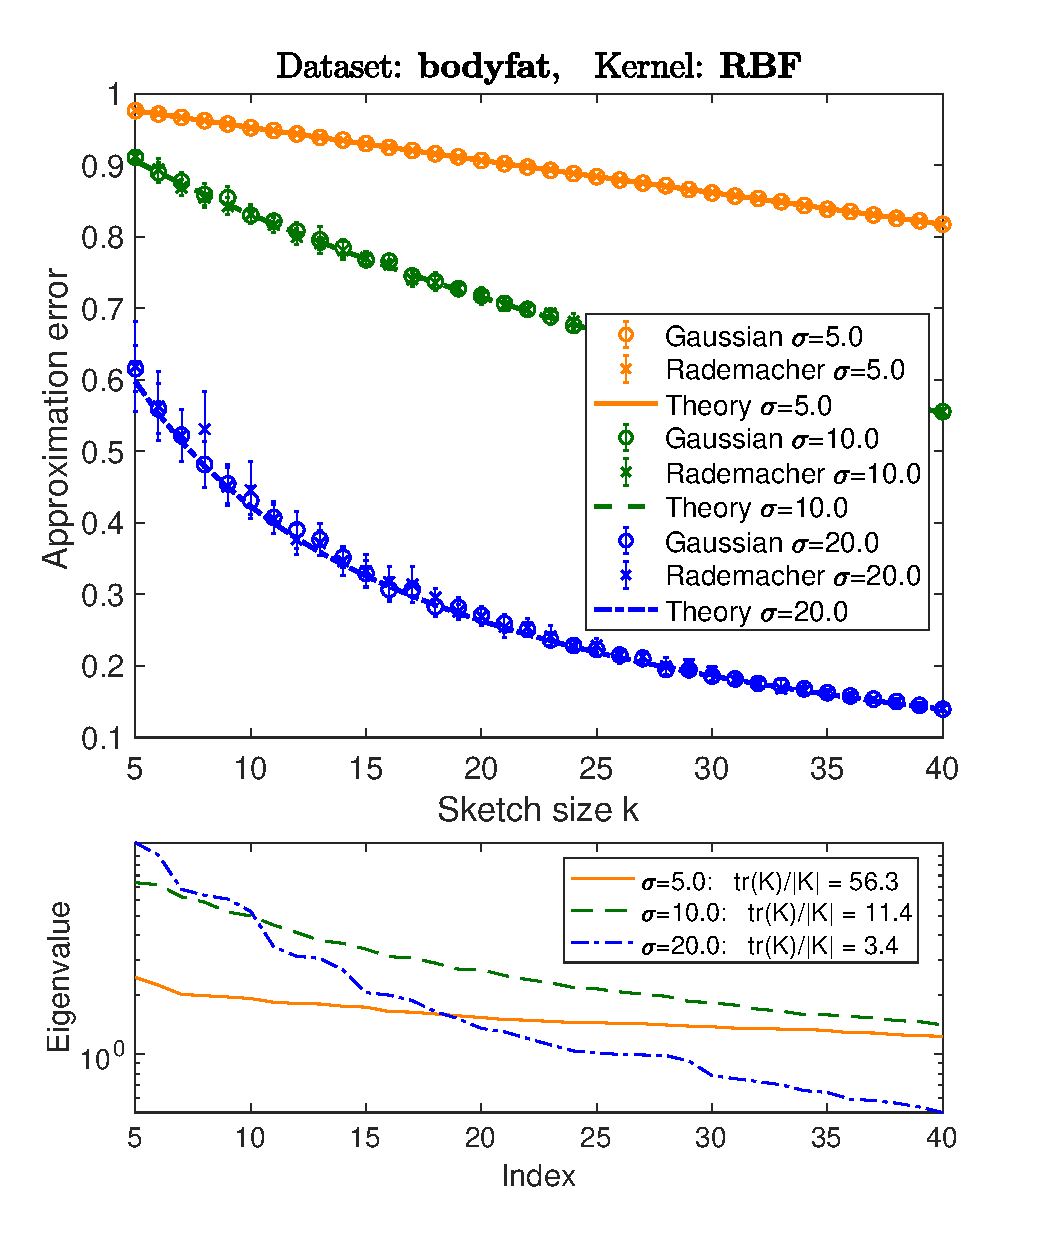
\includegraphics[width=.47\textwidth]{bodyfat-supp}\nobreak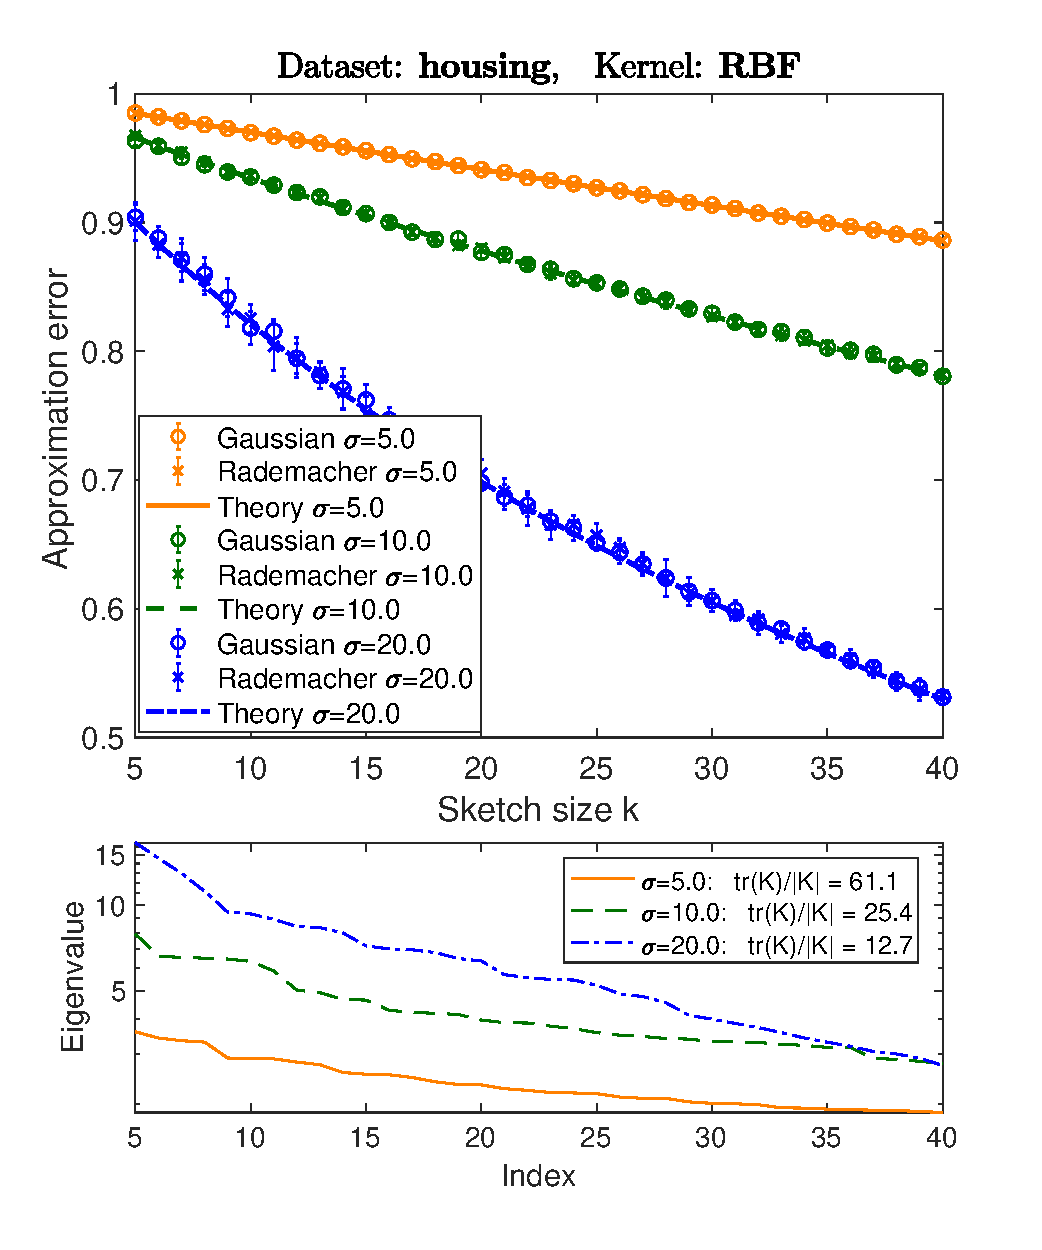
\includegraphics[width=.47\textwidth]{housing-supp}
  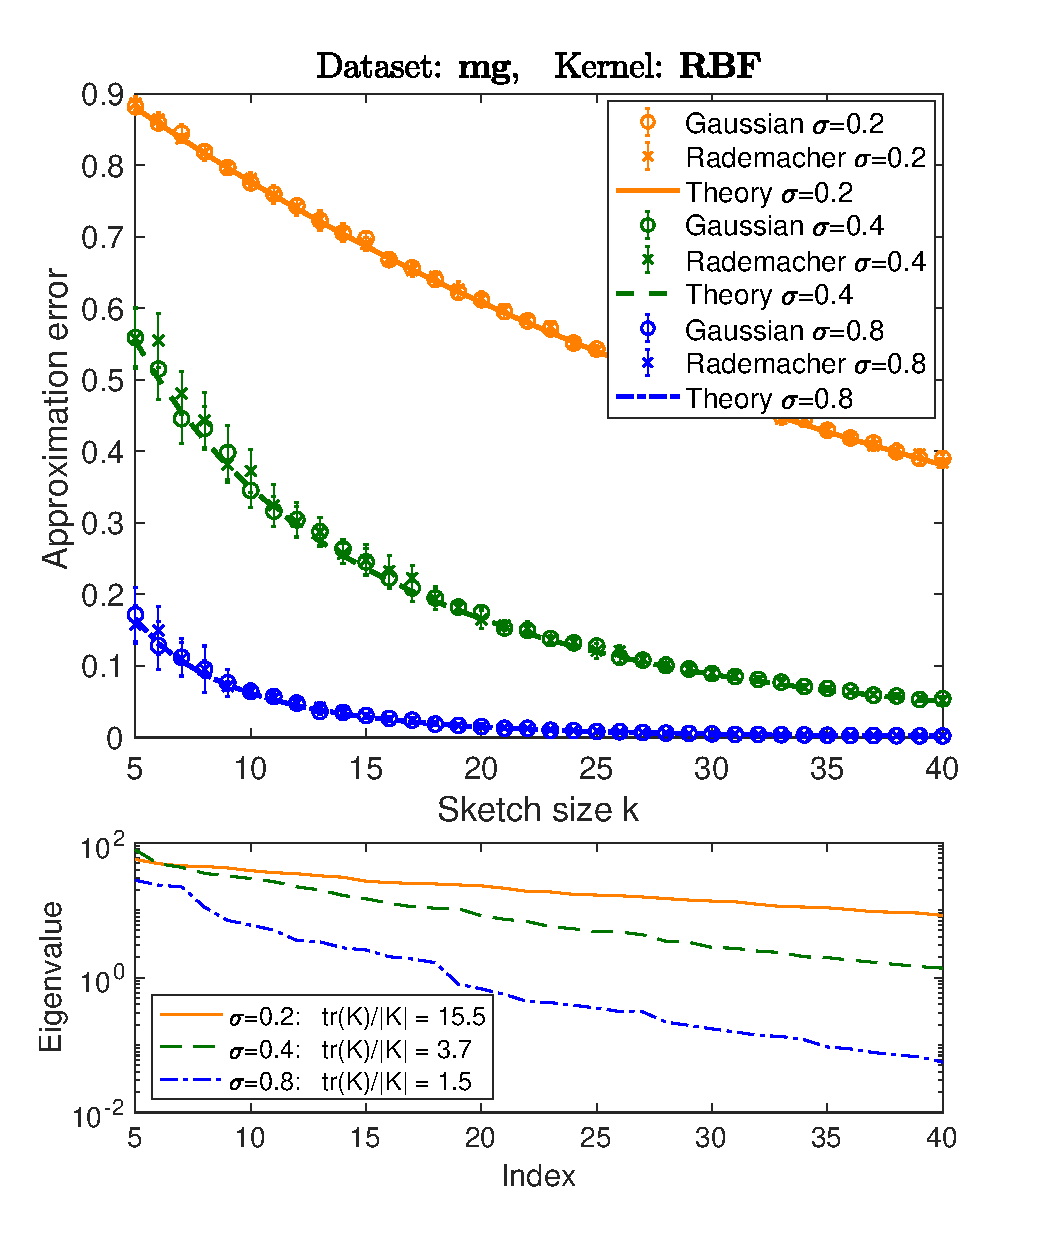
\includegraphics[width=.47\textwidth]{mg-supp}\nobreak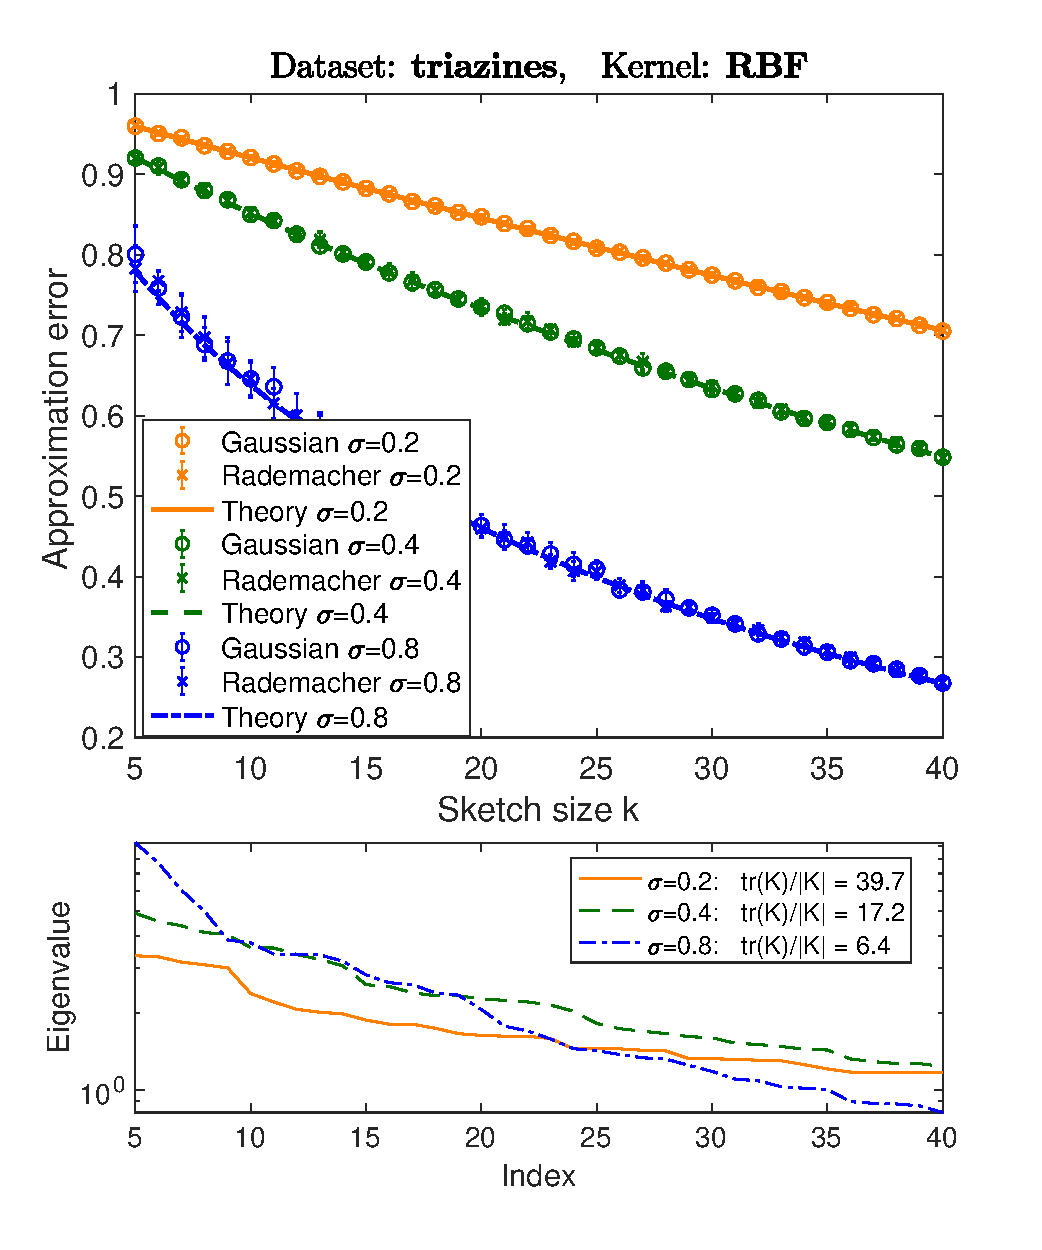
\includegraphics[width=.47\textwidth]{triazines-supp} 
  \caption{Theoretical predictions versus approximation error for the
    sketched Nystr\"om with the RBF kernel, using Gaussian and
    Rademacher sketches (spectral decay shown at the bottom).}\label{f:nystrom2}
\end{figure}

\section{Additional empirical results}
\label{a:experiments}

We complement the results of Section \ref{s:experiments} with
empirical results on four additional libsvm datasets \cite{libsvm} (bringing
the total number of benchmark datasets to eight), which further
establish the accuracy of our surrogate expressions for the low-rank approximation
error. Similary as in Figure \ref{f:nystrom}, we use the sketched
Nystr\"om method \cite{revisiting-nystrom} with the RBF kernel
$k(\a_i,\a_j)=\exp(-\|\a_i-\a_j\|^2/(2\sigma^2))$, for several values
of the parameter $\sigma$. The values of $\sigma$ were chosen so as to
demonstrate the effectiveness of our theoretical predictions both when the
stable rank is moderately large and when it is very small.

In Figure \ref{f:nystrom2} we show the results for both Gaussian and
Rademacher sketches. These results reinforce the conclusions we made in
Section \ref{s:experiments}: our theoretical estimates are very
accurate in all cases, for both sketching methods, and even when the
stable rank is close to 1 (a regime that is not supported by the
current theory).

\end{document}

% \begin{document}

% \maketitle

% \begin{abstract}
%   The abstract paragraph should be indented \nicefrac{1}{2}~inch (3~picas) on
%   both the left- and right-hand margins. Use 10~point type, with a vertical
%   spacing (leading) of 11~points.  The word \textbf{Abstract} must be centered,
%   bold, and in point size 12. Two line spaces precede the abstract. The abstract
%   must be limited to one paragraph.
% \end{abstract}

% \section{Submission of papers to NeurIPS 2020}

% NeurIPS requires electronic submissions.  The electronic submission site is
% \begin{center}
%   \url{https://cmt3.research.microsoft.com/NeurIPS2020/}
% \end{center}

% Please read the instructions below carefully and follow them faithfully.

% \subsection{Style}

% Papers to be submitted to NeurIPS 2020 must be prepared according to the
% instructions presented here. Papers may only be up to eight pages long,
% including figures. Additional pages \emph{containing only a section on the broader impact, acknowledgments and/or cited references} are allowed. Papers that exceed eight pages of content will not be reviewed, or in any other way considered for
% presentation at the conference.

% The margins in 2020 are the same as those in 2007, which allow for $\sim$$15\%$
% more words in the paper compared to earlier years.

% Authors are required to use the NeurIPS \LaTeX{} style files obtainable at the
% NeurIPS website as indicated below. Please make sure you use the current files
% and not previous versions. Tweaking the style files may be grounds for
% rejection.

% \subsection{Retrieval of style files}

% The style files for NeurIPS and other conference information are available on
% the World Wide Web at
% \begin{center}
%   \url{http://www.neurips.cc/}
% \end{center}
% The file \verb+neurips_2020.pdf+ contains these instructions and illustrates the
% various formatting requirements your NeurIPS paper must satisfy.

% The only supported style file for NeurIPS 2020 is \verb+neurips_2020.sty+,
% rewritten for \LaTeXe{}.  \textbf{Previous style files for \LaTeX{} 2.09,
%   Microsoft Word, and RTF are no longer supported!}

% The \LaTeX{} style file contains three optional arguments: \verb+final+, which
% creates a camera-ready copy, \verb+preprint+, which creates a preprint for
% submission to, e.g., arXiv, and \verb+nonatbib+, which will not load the
% \verb+natbib+ package for you in case of package clash.

% \paragraph{Preprint option}
% If you wish to post a preprint of your work online, e.g., on arXiv, using the
% NeurIPS style, please use the \verb+preprint+ option. This will create a
% nonanonymized version of your work with the text ``Preprint. Work in progress.''
% in the footer. This version may be distributed as you see fit. Please \textbf{do
%   not} use the \verb+final+ option, which should \textbf{only} be used for
% papers accepted to NeurIPS.

% At submission time, please omit the \verb+final+ and \verb+preprint+
% options. This will anonymize your submission and add line numbers to aid
% review. Please do \emph{not} refer to these line numbers in your paper as they
% will be removed during generation of camera-ready copies.

% The file \verb+neurips_2020.tex+ may be used as a ``shell'' for writing your
% paper. All you have to do is replace the author, title, abstract, and text of
% the paper with your own.

% The formatting instructions contained in these style files are summarized in
% Sections \ref{gen_inst}, \ref{headings}, and \ref{others} below.

% \section{General formatting instructions}
% \label{gen_inst}

% The text must be confined within a rectangle 5.5~inches (33~picas) wide and
% 9~inches (54~picas) long. The left margin is 1.5~inch (9~picas).  Use 10~point
% type with a vertical spacing (leading) of 11~points.  Times New Roman is the
% preferred typeface throughout, and will be selected for you by default.
% Paragraphs are separated by \nicefrac{1}{2}~line space (5.5 points), with no
% indentation.

% The paper title should be 17~point, initial caps/lower case, bold, centered
% between two horizontal rules. The top rule should be 4~points thick and the
% bottom rule should be 1~point thick. Allow \nicefrac{1}{4}~inch space above and
% below the title to rules. All pages should start at 1~inch (6~picas) from the
% top of the page.

% For the final version, authors' names are set in boldface, and each name is
% centered above the corresponding address. The lead author's name is to be listed
% first (left-most), and the co-authors' names (if different address) are set to
% follow. If there is only one co-author, list both author and co-author side by
% side.

% Please pay special attention to the instructions in Section \ref{others}
% regarding figures, tables, acknowledgments, and references.

% \section{Headings: first level}
% \label{headings}

% All headings should be lower case (except for first word and proper nouns),
% flush left, and bold.

% First-level headings should be in 12-point type.

% \subsection{Headings: second level}

% Second-level headings should be in 10-point type.

% \subsubsection{Headings: third level}

% Third-level headings should be in 10-point type.

% \paragraph{Paragraphs}

% There is also a \verb+\paragraph+ command available, which sets the heading in
% bold, flush left, and inline with the text, with the heading followed by 1\,em
% of space.

% \section{Citations, figures, tables, references}
% \label{others}

% These instructions apply to everyone.

% \subsection{Citations within the text}

% The \verb+natbib+ package will be loaded for you by default.  Citations may be
% author/year or numeric, as long as you maintain internal consistency.  As to the
% format of the references themselves, any style is acceptable as long as it is
% used consistently.

% The documentation for \verb+natbib+ may be found at
% \begin{center}
%   \url{http://mirrors.ctan.org/macros/latex/contrib/natbib/natnotes.pdf}
% \end{center}
% Of note is the command \verb+\citet+, which produces citations appropriate for
% use in inline text.  For example,
% \begin{verbatim}
%    \citet{hasselmo} investigated\dots
% \end{verbatim}
% produces
% \begin{quote}
%   Hasselmo, et al.\ (1995) investigated\dots
% \end{quote}

% If you wish to load the \verb+natbib+ package with options, you may add the
% following before loading the \verb+neurips_2020+ package:
% \begin{verbatim}
%    \PassOptionsToPackage{options}{natbib}
% \end{verbatim}

% If \verb+natbib+ clashes with another package you load, you can add the optional
% argument \verb+nonatbib+ when loading the style file:
% \begin{verbatim}
%    \usepackage[nonatbib]{neurips_2020}
% \end{verbatim}

% As submission is double blind, refer to your own published work in the third
% person. That is, use ``In the previous work of Jones et al.\ [4],'' not ``In our
% previous work [4].'' If you cite your other papers that are not widely available
% (e.g., a journal paper under review), use anonymous author names in the
% citation, e.g., an author of the form ``A.\ Anonymous.''

% \subsection{Footnotes}

% Footnotes should be used sparingly.  If you do require a footnote, indicate
% footnotes with a number\footnote{Sample of the first footnote.} in the
% text. Place the footnotes at the bottom of the page on which they appear.
% Precede the footnote with a horizontal rule of 2~inches (12~picas).

% Note that footnotes are properly typeset \emph{after} punctuation
% marks.\footnote{As in this example.}

% \subsection{Figures}

% \begin{figure}
%   \centering
%   \fbox{\rule[-.5cm]{0cm}{4cm} \rule[-.5cm]{4cm}{0cm}}
%   \caption{Sample figure caption.}
% \end{figure}

% All artwork must be neat, clean, and legible. Lines should be dark enough for
% purposes of reproduction. The figure number and caption always appear after the
% figure. Place one line space before the figure caption and one line space after
% the figure. The figure caption should be lower case (except for first word and
% proper nouns); figures are numbered consecutively.

% You may use color figures.  However, it is best for the figure captions and the
% paper body to be legible if the paper is printed in either black/white or in
% color.

% \subsection{Tables}

% All tables must be centered, neat, clean and legible.  The table number and
% title always appear before the table.  See Table~\ref{sample-table}.

% Place one line space before the table title, one line space after the
% table title, and one line space after the table. The table title must
% be lower case (except for first word and proper nouns); tables are
% numbered consecutively.

% Note that publication-quality tables \emph{do not contain vertical rules.} We
% strongly suggest the use of the \verb+booktabs+ package, which allows for
% typesetting high-quality, professional tables:
% \begin{center}
%   \url{https://www.ctan.org/pkg/booktabs}
% \end{center}
% This package was used to typeset Table~\ref{sample-table}.
%
% \begin{table}
%   \caption{Sample table title}
%   \label{sample-table}
%   \centering
%   \begin{tabular}{lll}
%     \toprule
%     \multicolumn{2}{c}{Part}                   \\
%     \cmidrule(r){1-2}
%     Name     & Description     & Size ($\mu$m) \\
%     \midrule
%     Dendrite & Input terminal  & $\sim$100     \\
%     Axon     & Output terminal & $\sim$10      \\
%     Soma     & Cell body       & up to $10^6$  \\
%     \bottomrule
%   \end{tabular}
% \end{table}
%
% \section{Final instructions}
%
% Do not change any aspects of the formatting parameters in the style files.  In
% particular, do not modify the width or length of the rectangle the text should
% fit into, and do not change font sizes (except perhaps in the
% \textbf{References} section; see below). Please note that pages should be
% numbered.
%
% \section{Preparing PDF files}
%
% Please prepare submission files with paper size ``US Letter,'' and not, for
% example, ``A4.''
%
% Fonts were the main cause of problems in the past years. Your PDF file must only
% contain Type 1 or Embedded TrueType fonts. Here are a few instructions to
% achieve this.
%
% \begin{itemize}
%
% \item You should directly generate PDF files using \verb+pdflatex+.
%
% \item You can check which fonts a PDF files uses.  In Acrobat Reader, select the
%   menu Files$>$Document Properties$>$Fonts and select Show All Fonts. You can
%   also use the program \verb+pdffonts+ which comes with \verb+xpdf+ and is
%   available out-of-the-box on most Linux machines.
%
% \item The IEEE has recommendations for generating PDF files whose fonts are also
%   acceptable for NeurIPS. Please see
%   \url{http://www.emfield.org/icuwb2010/downloads/IEEE-PDF-SpecV32.pdf}
%
% \item \verb+xfig+ "patterned" shapes are implemented with bitmap fonts.  Use
%   "solid" shapes instead.
%
% \item The \verb+\bbold+ package almost always uses bitmap fonts.  You should use
%   the equivalent AMS Fonts:
% \begin{verbatim}
%    \usepackage{amsfonts}
% \end{verbatim}
% followed by, e.g., \verb+\mathbb{R}+, \verb+\mathbb{N}+, or \verb+\mathbb{C}+
% for $\mathbb{R}$, $\mathbb{N}$ or $\mathbb{C}$.  You can also use the following
% workaround for reals, natural and complex:
% \begin{verbatim}
%    \newcommand{\RR}{I\!\!R} %real numbers
%    \newcommand{\Nat}{I\!\!N} %natural numbers
%    \newcommand{\CC}{I\!\!\!\!C} %complex numbers
% \end{verbatim}
% Note that \verb+amsfonts+ is automatically loaded by the \verb+amssymb+ package.
%
% \end{itemize}
%
% If your file contains type 3 fonts or non embedded TrueType fonts, we will ask
% you to fix it.
%
% \subsection{Margins in \LaTeX{}}
%
% Most of the margin problems come from figures positioned by hand using
% \verb+\special+ or other commands. We suggest using the command
% \verb+\includegraphics+ from the \verb+graphicx+ package. Always specify the
% figure width as a multiple of the line width as in the example below:
% \begin{verbatim}
%    \usepackage[pdftex]{graphicx} ...
%    \includegraphics[width=0.8\linewidth]{myfile.pdf}
% \end{verbatim}
% See Section 4.4 in the graphics bundle documentation
% (\url{http://mirrors.ctan.org/macros/latex/required/graphics/grfguide.pdf})
%
% A number of width problems arise when \LaTeX{} cannot properly hyphenate a
% line. Please give LaTeX hyphenation hints using the \verb+\-+ command when
% necessary.
%
%
% \section*{Broader Impact}
%
% Authors are required to include a statement of the broader impact of their work, including its ethical aspects and future societal consequences.
% Authors should discuss both positive and negative outcomes, if any. For instance, authors should discuss a)
% who may benefit from this research, b) who may be put at disadvantage from this research, c) what are the consequences of failure of the system, and d) whether the task/method leverages
% biases in the data. If authors believe this is not applicable to them, authors can simply state this.
%
% Use unnumbered first level headings for this section, which should go at the end of the paper. {\bf Note that this section does not count towards the eight pages of content that are allowed.}
%
% \begin{ack}
% Use unnumbered first level headings for the acknowledgments. All acknowledgments
% go at the end of the paper before the list of references. Moreover, you are required to declare
% funding (financial activities supporting the submitted work) and competing interests (related financial activities outside the submitted work).
% More information about this disclosure can be found at: \url{https://neurips.cc/Conferences/2020/PaperInformation/FundingDisclosure}.
%
%
% Do {\bf not} include this section in the anonymized submission, only in the final paper. You can use the \texttt{ack} environment provided in the style file to autmoatically hide this section in the anonymized submission.
% \end{ack}
%
% \section*{References}
%
% References follow the acknowledgments. Use unnumbered first-level heading for
% the references. Any choice of citation style is acceptable as long as you are
% consistent. It is permissible to reduce the font size to \verb+small+ (9 point)
% when listing the references.
% {\bf Note that the Reference section does not count towards the eight pages of content that are allowed.}
% \medskip
%
% \small
%
% [1] Alexander, J.A.\ \& Mozer, M.C.\ (1995) Template-based algorithms for
% connectionist rule extraction. In G.\ Tesauro, D.S.\ Touretzky and T.K.\ Leen
% (eds.), {\it Advances in Neural Information Processing Systems 7},
% pp.\ 609--616. Cambridge, MA: MIT Press.
%
% [2] Bower, J.M.\ \& Beeman, D.\ (1995) {\it The Book of GENESIS: Exploring
%   Realistic Neural Models with the GEneral NEural SImulation System.}  New York:
% TELOS/Springer--Verlag.
%
% [3] Hasselmo, M.E., Schnell, E.\ \& Barkai, E.\ (1995) Dynamics of learning and
% recall at excitatory recurrent synapses and cholinergic modulation in rat
% hippocampal region CA3. {\it Journal of Neuroscience} {\bf 15}(7):5249-5262.
%
% \end{document}
